%%%%%%%%%%%%%%%%%%%%%%%%%%%%%%%%%%%%%%%%%
% The Legrand Orange Book
% LaTeX Template
% Version 3.1 (February 18, 2022)
%
% This template originates from:
% https://www.LaTeXTemplates.com
%
% Authors:
% Vel (vel@latextemplates.com)
% Mathias Legrand (legrand.mathias@gmail.com)
%
% License:
% CC BY-NC-SA 4.0 (https://creativecommons.org/licenses/by-nc-sa/4.0/)
%
% Compiling this template:
% This template uses biber for its bibliography and makeindex for its index.
% When you first open the template, compile it from the command line with the 
% commands below to make sure your LaTeX distribution is configured correctly:
%
% 1) pdflatex main
% 2) makeindex main.idx -s indexstyle.ist
% 3) biber main
% 4) pdflatex main x 2
%
% After this, when you wish to update the bibliography/index use the appropriate
% command above and make sure to compile with pdflatex several times 
% afterwards to propagate your changes to the document.
%
%%%%%%%%%%%%%%%%%%%%%%%%%%%%%%%%%%%%%%%%%

%----------------------------------------------------------------------------------------
%	PACKAGES AND OTHER DOCUMENT CONFIGURATIONS
%----------------------------------------------------------------------------------------

\documentclass[
	11pt, % Default font size, select one of 10pt, 11pt or 12pt
	fleqn, % Left align equations
	a4paper, % Paper size, use either 'a4paper' for A4 size or 'letterpaper' for US letter size
	%oneside, % Uncomment for oneside mode, this doesn't start new chapters and parts on odd pages (adding an empty page if required), this mode is more suitable if the book is to be read on a screen instead of printed
]{LegrandOrangeBook}

% Book information for PDF metadata, remove/comment this block if not required 
\hypersetup{
	pdftitle={Title}, % Title field
	pdfauthor={Author}, % Author field
	pdfsubject={Subject}, % Subject field
	pdfkeywords={Keyword1, Keyword2, ...}, % Keywords
	pdfcreator={LaTeX}, % Content creator field
}

\addbibresource{sample.bib} % Bibliography file

\definecolor{ocre}{RGB}{243, 102, 25} % Define the color used for highlighting throughout the book
% \definecolor{ocre}{RGB}{0, 0, 0} % Define the color used for highlighting throughout the book

\chapterimage{orange1.jpg} % Chapter heading image
\chapterspaceabove{6.5cm} % Default whitespace from the top of the page to the chapter title on chapter pages
\chapterspacebelow{6.75cm} % Default amount of vertical whitespace from the top margin to the start of the text on chapter pages

%----------------------------------------------------------------------------------------
%	以下是我们自己添加的额外packages
%----------------------------------------------------------------------------------------

% ******** Eye Protection 保护眼睛 ********
\usepackage{xcolor} % For defining and using colors
\definecolor{mygreen}{RGB}{205, 222, 194} % Define a custom green color for eye protection
% \pagecolor{mygreen} % Set page background color to custom green
% *****************************************

\usepackage[colorinlistoftodos]{todonotes}

%贺立添加的包--------------------------------------------------------------
\usepackage{graphicx} % Required for inserting images
\usepackage{quantikz}
\usepackage[utf8]{inputenc}
\usepackage[english]{babel}
\usepackage{amsthm}
\usepackage{mdframed}
\usepackage{xcolor}
\usepackage{ulem}
\usepackage[thicklines]{cancel}
\usepackage{tocbibind} % 加载宏包以添加目录到目录中
\usepackage{caption}
\captionsetup[figure]{labelsep=space}

% 定义自定义的方框样式
\mdfdefinestyle{mystyle}{
	roundcorner=10pt,
	backgroundcolor=blue!10,
	frametitlerule=true,
	frametitlebackgroundcolor=blue!20,
}
%----------------------------------------------------------------------

%\newtheorem{theorem}{Theorem}
%\newtheorem{remark}{Remark}
%\newtheorem{property}{Property}
%\newtheorem{definition}{Definition}
%\newtheorem{example}{Example}
%\newtheorem{corollary}{Corollary}
%\newtheorem{lemma}{Lemma}
%\newtheorem{postulate}{Postulate}
%\newtheorem{proposition}{Proposition}
%\renewcommand{\thefootnote}{\fnsymbol{footnote}} %注脚符号的注脚方式



\begin{document}

%----------------------------------------------------------------------------------------
%	TITLE PAGE
%----------------------------------------------------------------------------------------

\titlepage % Output the title page
	{
\includegraphics[width=\paperwidth]{background.pdf}} % Code to output the background image, which should be the same dimensions as the paper to fill the page entirely; leave empty for no background image
	{ % Title(s) and author(s)
		\centering\sffamily % Font styling
		{\Huge\bfseries
            Quantum Computation and Optimization
            \par} % Book title
		\vspace{16pt} % Vertical whitespace
		{\LARGE A Study Note\par} % Subtitle
		\vspace{24pt} % Vertical whitespace
		{\huge\bfseries
            Zhijian Lai, 
            Jiang Hu, 
            Li He
            \par} % Author name
	}

% %----------------------------------------------------------------------------------------
% %	COPYRIGHT PAGE
% %----------------------------------------------------------------------------------------

% \thispagestyle{empty} % Suppress headers and footers on this page

% ~\vfill % Push the text down to the bottom of the page

% \noindent Copyright \copyright\ 2022 Goro Akechi\\ % Copyright notice

% \noindent \textsc{Published by Publisher}\\ % Publisher

% \noindent \textsc{\href{https://www.latextemplates.com/template/legrand-orange-book}{book-website.com}}\\ % URL

% \noindent Licensed under the Creative Commons Attribution-NonCommercial 4.0 License (the ``License''). You may not use this file except in compliance with the License. You may obtain a copy of the License at \url{https://creativecommons.org/licenses/by-nc-sa/4.0}. Unless required by applicable law or agreed to in writing, software distributed under the License is distributed on an \textsc{``as is'' basis, without warranties or conditions of any kind}, either express or implied. See the License for the specific language governing permissions and limitations under the License.\\ % License information, replace this with your own license (if any)

% \noindent \textit{First printing, March 2022} % Printing/edition date

%----------------------------------------------------------------------------------------
%	TABLE OF CONTENTS
%----------------------------------------------------------------------------------------

\pagestyle{empty} % Disable headers and footers for the following pages

\tableofcontents % Output the table of contents

% \listoffigures % Output the list of figures, comment or remove this command if not required

% \listoftables % Output the list of tables, comment or remove this command if not required

\pagestyle{fancy} % Enable default headers and footers again

\cleardoublepage % Start the following content on a new page

%----------------------------------------------------------------------------------------
%	SECTIONING EXAMPLES CHAPTER
%----------------------------------------------------------------------------------------

\chapterimage{orange2.jpg} % Chapter heading image
\chapterspaceabove{6.75cm} % Whitespace from the top of the page to the chapter title on chapter pages
\chapterspacebelow{7.25cm} % Amount of vertical whitespace from the top margin to the start of the text on chapter pages

%------------------------------------------------

 

% ==========================  正文开始  ==========================

%----------------------------------------------------------------------------------------
%	PART I
%----------------------------------------------------------------------------------------

\part{Notes of NC book}

\chapter{Introduction to quantum mechanics}

\section{Linear algebra}

A good understanding of quantum mechanics is based upon a solid grasp of linear algebra.

%   1.1.1 vector space
\subsection{vector space}
The vector space of most interest to us is $\mathbf{C}^{n}$, the space of all $n$-tuples of complex numbers, $\left(z_{1}, \ldots, z_{n}\right)$. The elements of a vector space are called vectors, and we will sometimes use the column matrix notation
$$
\left[\begin{array}{c}
z_{1} \\
\vdots \\
z_{n}
\end{array}\right]
$$
to indicate a vector. For convenience, we use the notation $\left(z_{1}, \ldots, z_{n}\right)$ to denote a column matrix with entries $z_{1}, \ldots, z_{n}$. 

There is an addition operation defined which takes pairs of vectors to other vectors. In $\mathbf{C}^{n}$ the addition operation for vectors is defined by
$$
\left[\begin{array}{c}
z_{1} \\
\vdots \\
z_{n}
\end{array}\right]+\left[\begin{array}{c}
z_{1}^{\prime} \\
\vdots \\
z_{n}^{\prime}
\end{array}\right] \equiv\left[\begin{array}{c}
z_{1}+z_{1}^{\prime} \\
\vdots \\
z_{n}+z_{n}^{\prime}
\end{array}\right]
$$
where the addition operations on the right are just ordinary additions of complex numbers. Furthermore, in a vector space there is a scalar multiplication operation. In $\mathbf{C}^{n}$ this is defined by
$$
z\left[\begin{array}{c}
z_{1} \\
\vdots \\
z_{n}
\end{array}\right] \equiv\left[\begin{array}{c}
z z_{1} \\
\vdots \\
z z_{n}
\end{array}\right]
$$
where $z$ is a scalar, that is, a complex number\footnote{Physicists sometimes refer to complex numbers as $c$-numbers.}, and the multiplications on the right are ordinary multiplication of complex numbers. A vector subspace of a vector space $V$ is a subset $W$ of $V$ such that $W$ is also a vector space, that is, $W$ must be closed under scalar multiplication and addition.

We will use the \textit{standard} notation of quantum mechanics for linear algebraic concepts, see Figure \ref{tab:summary_AL}. For a vector in a vector space is the following:
$$
|\psi\rangle .
$$
The notation $|\cdot\rangle$, called "ket", is used to indicate that the object is a (column) vector, and $\psi$ is a label for the vector. The entire object $|\psi\rangle$ is pronounced  as "ket psi". Any label is valid, although we prefer to use simple labels like $\psi$ and $\varphi$.

\begin{remark} %zero vector $0$ and the special vector $|0\rangle$
    A vector space also contains a special zero vector, which we denote by 0. In $\mathbf{C}^{n}$ the zero element is $0=(0,0, \ldots, 0)$. Note that we do not use the ket notation for the zero vector - it is the only exception we shall make. Because, it is conventional to use the notation $|0\rangle$ to mean some special vector that is not zero vector.
\end{remark}

\begin{table}[]
    \centering
    \begin{tabular}{c|l}
        \hline\hline
        Notation & Description \\
        \hline
        $z^{*}$ & Complex conjugate of the complex number $z$. $(1+i)^{*}=1-i$\\
        $|\psi\rangle$& Vector. Also known as a ket. \\
        $\langle\psi|$& Vector dual to $|\psi\rangle$. Also known as a bra. \\
        $\langle\varphi | \psi\rangle$& Inner product between the vectors $|\varphi\rangle$ and $|\psi\rangle$. \\
        $|\varphi\rangle \otimes|\psi\rangle$& Tensor product of $|\varphi\rangle$ and $|\psi\rangle$. \\
        $|\varphi\rangle|\psi\rangle$& Abbreviated notation for tensor product of $|\varphi\rangle$ and $|\psi\rangle$. \\
        $A^{*}$& Complex conjugate of the $A$ matrix. \\
        $A^{T}$& Transpose of the $A$ matrix. \\
         $A^{\dagger}$& Hermitian conjugate or adjoint of the $A$ matrix, $A^{\dagger}=\left(A^{T}\right)^{*}$. \\
         & $\left[\begin{array}{cc}a & b \\ c & d\end{array}\right]^{\dagger}=\left[\begin{array}{cc}a^{*} & c^{*} \\ b^{*} & d^{*}\end{array}\right]$. \\
        $\langle\varphi|A| \psi\rangle$ & Inner product between $|\varphi\rangle$ and $A|\psi\rangle$. \\
         & Equivalently, inner product between $A^{\dagger}|\varphi\rangle$ and $|\psi\rangle$. \\
        \hline\hline
    \end{tabular}
\caption{Summary of some standard quantum mechanical notation for notions from linear algebra. This style of notation is known as the Dirac notation.}
\label{tab:summary_AL}
\end{table}

%   1.1.2 Bases and linear independence
\subsection{Bases and linear independence}
A spanning set for a vector space is a set of vectors $\left|v_{1}\right\rangle, \ldots,\left|v_{n}\right\rangle$ such that any vector $|v\rangle$ in the vector space can be written as a linear combination $|v\rangle=\sum_{i} a_{i}\left|v_{i}\right\rangle$ of vectors in that set. 

\begin{example}
    For example, a spanning set for the vector space $\mathbf{C}^{2}$ is the set
    $$
    \left|v_{1}\right\rangle \equiv\left[\begin{array}{l}
    1 \\
    0
    \end{array}\right] ; \quad\left|v_{2}\right\rangle  \equiv\left[\begin{array}{l}
    0 \\
    1
    \end{array}\right]
  $$
    since any vector
    $$
    |v\rangle=\left[\begin{array}{l}
    a_{1} \\
    a_{2}
    \end{array}\right]
    $$
    in $\mathbf{C}^{2}$ can be written as a linear combination $|v\rangle=a_{1}\left|v_{1}\right\rangle+a_{2}\left|v_{2}\right\rangle$ of the vectors $\left|v_{1}\right\rangle$ and $\left|v_{2}\right\rangle$. We say that the vectors $\left|v_{1}\right\rangle$ and $\left|v_{2}\right\rangle$ span the vector space $\mathbf{C}^{2}$.
\end{example}

Generally, a vector space may have many different spanning sets. 

\begin{example}
A second spanning set for the vector space $\mathbf{C}^{2}$ is the set
$$
\left|v_{1}\right\rangle \equiv \frac{1}{\sqrt{2}}\left[\begin{array}{l}
1 \\
1
\end{array}\right] ; \quad\left|v_{2}\right\rangle \equiv \frac{1}{\sqrt{2}}\left[\begin{array}{r}
1 \\
-1
\end{array}\right]
$$
since an arbitrary vector $|v\rangle=\left(a_{1}, a_{2}\right)$ can be written as a linear combination of $\left|v_{1}\right\rangle$ and $\left|v_{2}\right\rangle$,
$$
|v\rangle=\frac{a_{1}+a_{2}}{\sqrt{2}}\left|v_{1}\right\rangle+\frac{a_{1}-a_{2}}{\sqrt{2}}\left|v_{2}\right\rangle.
$$
\end{example}

A set of non-zero vectors $\left|v_{1}\right\rangle, \ldots,\left|v_{n}\right\rangle$ are linearly dependent if there exists a set of complex numbers $a_{1}, \ldots, a_{n}$ with $a_{i} \neq 0$ for at least one value of $i$, such that
$$
a_{1}\left|v_{1}\right\rangle+a_{2}\left|v_{2}\right\rangle+\cdots+a_{n}\left|v_{n}\right\rangle=0.
$$
A set of vectors is linearly independent if it is not linearly dependent. 

It can be shown that any two sets of linearly independent vectors which span a vector space $V$ contain the same number of elements. We call such a set a basis for $V$. Furthermore, such a basis set always exists. The number of elements in the basis is defined to be the dimension of $V$. In this book we will only be interested in finite dimensional vector spaces. 

% Exercise 2.1: (Linear dependence: example) Show that $(1,-1),(1,2)$ and $(2,1)$ are linearly dependent.

%   1.1.3 Linear operators and matrices
\subsection{Linear operators and matrices}
A linear operator between vector spaces $V$ and $W$ is defined to be a function $A$ : $V \rightarrow W$ which is linear in its inputs,
\begin{equation}\label{eq:linear-operator}
A\left(\sum_{i} a_{i}\left|v_{i}\right\rangle\right)=\sum_{i} a_{i} A\left(\left|v_{i}\right\rangle\right).
\end{equation}
Usually we just write $A|v\rangle$ to denote $A(|v\rangle)$. When we say that a linear operator $A$ is defined on a vector space, $V$, we mean that $A$ is a linear operator from $V$ to $V$. 

\begin{example}
    An important linear operator on any vector space $V$ is the identity operator, $I_{V}$, defined by the equation $I_{V}|v\rangle \equiv|v\rangle$ for all vectors $|v\rangle$. Where no chance of confusion arises we drop the subscript $V$ and just write $I$ to denote the identity operator. 
\end{example}

\begin{example}
    Another important linear operator is the zero operator, which we denote 0 . The zero operator maps all vectors to the zero vector, $0|v\rangle \equiv 0$. 
\end{example}

It is clear from (\ref{eq:linear-operator}) that once the action of a linear operator $A$ on a basis (of its domain) is specified, the action of $A$ is completely determined on all inputs. This tells us that, when we want to show that two linear operators $A,B:V \rightarrow W$ are the same, we only need to show that $A |v_{i}\rangle = B|v_{i}\rangle$ holds for all $i$ under an arbitrary basis $\{|v_{i}\rangle\}$ of $V.$

Suppose $V, W$, and $X$ are vector spaces, and $A: V \rightarrow W$ and $B: W \rightarrow X$ are linear operators. Then we use the notation $B A$ to denote the composition of $B$ with $A$, defined by $(B A)(|v\rangle) \equiv B(A(|v\rangle))$. Once again, we write $B A|v\rangle$ as an abbreviation for $(B A)(|v\rangle)$.

The most convenient way to understand linear operators is in terms of their matrix representations. In fact, the linear operator and matrix viewpoints turn out to be completely equivalent. 

\paragraph{Every matrix can be regarded as a linear operator}
To see the connection, it helps to first understand that an $m$ by $n$ complex matrix $A$ with entries $A_{i j}$ is in fact a linear operator sending vectors in the vector space $\mathbf{C}^{n}$ to the vector space $\mathbf{C}^{m}$, under matrix multiplication of the matrix $A$ by a vector in $\mathbf{C}^{n}$. We've seen that matrices can be regarded as linear operators.

\paragraph{Every linear operator can be given a matrix representation}
Suppose $A: V \rightarrow W$ is a linear operator between vector spaces $V$ and $W$. Suppose $\left|v_{1}\right\rangle, \ldots,\left|v_{m}\right\rangle$ is a basis for $V$ and $\left|w_{1}\right\rangle, \ldots,\left|w_{n}\right\rangle$ is a basis for $W$. Then for each $j$ in the range $1, \ldots, m$, there exist complex numbers $A_{1 j}, \dots, A_{n j}$ such that
$$
A\left|v_{j}\right\rangle=\sum_{i} A_{i j}\left|w_{i}\right\rangle.
$$
The matrix whose entries are the values $A_{i j}$ is said to form a matrix representation of the operator $A$. This matrix representation of $A$ is completely equivalent to the operator $A$, and we will use the matrix representation and abstract operator viewpoints interchangeably. 

% This equivalence between the two viewpoints justifies our interchanging terms from matrix theory and operator theory throughout the book. 

% Note that to make the connection between matrices and linear operators we must specify a set of input and output basis states for the input and output vector spaces of the linear operator.

\begin{exercise}
Exercise 2.2: (Matrix representations: example) Suppose $V$ is a vector space with basis vectors $|0\rangle$ and $|1\rangle$, and $A$ is a linear operator from $V$ to $V$ such that $A|0\rangle=|1\rangle$ and $A|1\rangle=|0\rangle$. Give a matrix representation for $A$, with respect to the input basis $|0\rangle,|1\rangle$, and the output basis $|0\rangle,|1\rangle$. Find input and output bases which give rise to a different matrix representation of $A$.
\end{exercise}

\begin{exercise}
Exercise 2.3: (Matrix representation for operator products) Suppose $A$ is a linear operator from vector space $V$ to vector space $W$, and $B$ is a linear operator from vector space $W$ to vector space $X$. Let $\left|v_{i}\right\rangle,\left|w_{j}\right\rangle$, and $\left|x_{k}\right\rangle$ be bases for the vector spaces $V, W$, and $X$, respectively. Show that the matrix representation for the linear transformation $B A$ is the matrix product of the matrix representations for $B$ and $A$, with respect to the appropriate bases.
\end{exercise}

\begin{exercise}
Exercise 2.4: (Matrix representation for identity) Show that the identity operator on a vector space $V$ has a matrix representation which is one along the diagonal and zero everywhere else, if the matrix representation is taken with respect to the same input and output bases. This matrix is known as the identity matrix.
\end{exercise}

%   1.1.4 The Pauli matrices
\subsection{The Pauli matrices}
%原2.1.3

Four extremely useful matrices which we shall often have occasion to use are the Pauli matrices. These are 2 by 2 matrices, which go by a variety of notations. The matrices, and their corresponding notations, are depicted in Figure 2.2. 


The Pauli matrices are so useful in the study of quantum computation and quantum information.

$$
\begin{aligned}
\sigma_{0} \equiv I \equiv\left[\begin{array}{rr}
1 & 0 \\
0 & 1
\end{array}\right] & \sigma_{1} \equiv \sigma_{x} \equiv X \equiv\left[\begin{array}{rr}
0 & 1 \\
1 & 0
\end{array}\right] \\
\sigma_{2} \equiv \sigma_{y} \equiv Y \equiv\left[\begin{array}{rr}
0 & -i \\
i & 0
\end{array}\right] & \sigma_{3} \equiv \sigma_{z} \equiv Z \equiv\left[\begin{array}{rr}
1 & 0 \\
0 & -1
\end{array}\right]
\end{aligned}
$$

Figure 2.2. The Pauli matrices. Sometimes $I$ is omitted from the list with just $X, Y$ and $Z$ known as the Pauli matrices.

%   1.1.5 Inner products
\subsection{Inner products}
%原2.1.4

% An inner product is a function which takes as input two vectors $|v\rangle$ and $|w\rangle$ from a vector space and produces a complex number as output. 

% We will see shortly that the matrix representation of dual vectors is just a row vector.

A function $(\cdot, \cdot)$ from $V \times V$ to $\mathbf{C}$ is an inner product if it satisfies the requirements that:
\begin{enumerate}
    \item $(\cdot, \cdot)$ is linear in the \textit{second} argument, 
$$
\left(|v\rangle, \sum_{i} \lambda_{i}\left|w_{i}\right\rangle\right)=\sum_{i} \lambda_{i}\left(|v\rangle,\left|w_{i}\right\rangle\right)
$$
    \item $(|v\rangle,|w\rangle)=(|w\rangle,|v\rangle)^{*}$.
    \item $(|v\rangle,|v\rangle) \geq 0$ with equality if and only if $|v\rangle=0$.
\end{enumerate}
We call a vector space equipped with an inner product an inner product space.

\begin{example}
    For example, $\mathbf{C}^{n}$ has an inner product defined by
$$
\left(\left(y_{1}, \ldots, y_{n}\right),\left(z_{1}, \ldots, z_{n}\right)\right) \equiv \sum_{i} y_{i}^{*} z_{i}=\left[y_{1}^{*} \ldots y_{n}^{*}\right]\left[\begin{array}{c}
z_{1} \\
\vdots \\
z_{n}
\end{array}\right].
$$
\end{example}

The standard quantum mechanical notation for the inner product $(|v\rangle,|w\rangle)$ is $$\langle v | w\rangle,$$where $|v\rangle$ and $|w\rangle$ are vectors in the inner product space, and the notation $\langle v|$ is used for the \textit{dual vector} to the vector $|v\rangle$; the dual is a linear operator from the inner product space $V$ to the complex numbers $\mathbf{C}$, defined by
$$
\langle v|(|w\rangle) \equiv\langle v | w\rangle \equiv(|v\rangle,|w\rangle).
$$

% Exercise 2.5: Verify that $(\cdot, \cdot)$ just defined is an inner product on $\mathbf{C}^{n}$.

\begin{exercise}
    Exercise 2.6: Show that any inner product $(\cdot, \cdot)$ is conjugate-linear in the \textit{first} argument\footnote{In some textbook of linear algebra, by definition they let inner product satisfy the linearity in the first argument. Then, like Exercise 2.6, we can show it is conjugate-linear in the second argument. Those two types of ways of definitions are indeed equivalent. },
$$
\left(\sum_{i} \lambda_{i}\left|w_{i}\right\rangle,|v\rangle\right)=\sum_{i} \lambda_{i}^{*}\left(\left|w_{i}\right\rangle,|v\rangle\right) .
$$
\end{exercise}

Discussions of quantum mechanics often refer to Hilbert space. In the finite dimensional complex vector spaces, a Hilbert space is exactly the same thing as an inner product space. From now on we use the two terms interchangeably, preferring the term Hilbert space.

% For example, $|w\rangle \equiv$ $(1,0)$ and $|v\rangle \equiv(0,1)$ are orthogonal with respect to the inner product defined by (2.14). 

We define the norm of a vector $|v\rangle$ by
$$
\||v\rangle \| \equiv \sqrt{\langle v | v\rangle}.
$$
A unit vector is a vector $|v\rangle$ such that $\||v\rangle \|=1$. We also say that $|v\rangle$ is normalized if $\| v\rangle \|=1$. It is convenient to talk of normalizing a vector by dividing by its norm; thus $|v\rangle / \||v\rangle \|$ is the normalized form of $|v\rangle$, for any non-zero vector $|v\rangle$. 
Vectors $|w\rangle$ and $|v\rangle$ are orthogonal if their inner product is zero. A set $|i\rangle$ of vectors with index $i$ is orthonormal if each vector is a unit vector, and distinct vectors in the set are orthogonal, that is, $\langle i | j\rangle=\delta_{i j}$, where $i$, $j$ are both chosen from the index set.

% Exercise 2.7: Verify that $|w\rangle \equiv(1,1)$ and $|v\rangle \equiv(1,-1)$ are orthogonal. What are the normalized forms of these vectors?

\begin{proposition}[Gram-Schmidt procedure]
    Suppose $\left|w_{1}\right\rangle, \ldots,\left|w_{d}\right\rangle$ is a basis set for some vector space $V$ with an inner product. There is a useful method, the Gram-Schmidt procedure, which can be used to produce an orthonormal basis set $\left|v_{1}\right\rangle, \ldots,\left|v_{d}\right\rangle$ for the vector space $V$. Define $\left|v_{1}\right\rangle \equiv\left|w_{1}\right\rangle / \|\left|w_{1}\right\rangle \|$, and for $1 \leq k \leq d-1$ define $\left|v_{k+1}\right\rangle$ inductively by
$$
\left|v_{k+1}\right\rangle \equiv \frac{\left|w_{k+1}\right\rangle-\sum_{i=1}^{k}\left\langle v_{i} | w_{k+1}\right\rangle\left|v_{i}\right\rangle}{\|\left|w_{k+1}\right\rangle-\sum_{i=1}^{k}\left\langle v_{i} | w_{k+1}\right\rangle\left|v_{i}\right\rangle \|}.
$$
\end{proposition}

It is not difficult to verify that the vectors $\left|v_{1}\right\rangle, \ldots,\left|v_{d}\right\rangle$ above form an orthonormal set which is also a basis for $V$. Thus, any finite dimensional vector space of dimension $d$ has an orthonormal basis, $\left|v_{1}\right\rangle, \ldots,\left|v_{d}\right\rangle$.

% Exercise 2.8: Prove that the Gram-Schmidt procedure produces an orthonormal basis for $V$.

\begin{remark}
    From now on, when we speak of a matrix representation for a linear operator, we mean a matrix representation with respect to orthonormal input and output bases. We also use the convention that if the input and output spaces for a linear operator are the same, then the input and output bases are the same, unless noted otherwise.
\end{remark}

With these conventions, the inner product on a Hilbert space can be given a convenient matrix representation. 

Let $|w\rangle=\sum_{i} w_{i}|i\rangle$ and $|v\rangle=\sum_{j} v_{j}|j\rangle$ be representations of vectors $|w\rangle$ and $|v\rangle$ with respect to some same orthonormal basis. Then, since $\langle i | j\rangle=\delta_{i j}$, we have
$$
\langle v | w\rangle 
=\left(\sum_{i} v_{i}|i\rangle, \sum_{j} w_{j}|j\rangle\right)=\sum_{i j} v_{i}^{*} w_{j} \delta_{i j}
=\sum_{i} v_{i}^{*} w_{i}
=\left[v_{1}^{*} \ldots v_{n}^{*}\right]\left[\begin{array}{c}
w_{1} \\
\vdots \\
w_{n}
\end{array}\right].
$$
That is, the inner product of two vectors is equal to the vector inner product between two matrix representations of those vectors, provided the representations are written with respect to the same orthonormal basis. 

% We also see that the dual vector $\langle v|$ has a nice interpretation as the row vector whose components are complex conjugates of the corresponding components of the column vector representation of $|v\rangle$.

%   1.1.6 Outer product
\subsection{Outer product}
%原2.1.4

% There is a useful way of representing linear operators which makes use of the inner product, known as the outer product representation. 

Suppose $|v\rangle$ is a vector in an inner product space $V$, and $|w\rangle$ is a vector in an inner product space $W$. Define the outer product of $|v\rangle$ and $|w\rangle$, denoted by $|w\rangle\langle v|$, to be the linear operator from $V$ to $W$:
$$
(|w\rangle\langle v|)\left(\left|v^{\prime}\right\rangle\right) \equiv|w\rangle\left\langle v | v^{\prime}\right\rangle=\left\langle v | v^{\prime}\right\rangle|w\rangle.
$$
Moreover, we define $\sum_{i} a_{i}\left|w_{i}\right\rangle\left\langle v_{i}\right|$ to be the linear operator which, when acting on $\left|v^{\prime}\right\rangle$, produces $\sum_{i} a_{i}\left|w_{i}\right\rangle\left\langle v_{i} | v^{\prime}\right\rangle$ as output.

The usefulness of the outer product notation can be discerned from an important result known as the completeness relation for orthonormal vectors. 

\begin{theorem}[Completeness relation of orthonormal basis]
    Let $|i\rangle$ be any orthonormal basis for the vector space $V$. Then, it follows that
$$
\sum_{i}|i\rangle\langle i|=I,
$$
which is called the completeness relation of orthonormal basis.
\end{theorem}
    
\begin{proof}
    Let $|i\rangle$ be any orthonormal basis for the vector space $V$, so an arbitrary vector $|v\rangle$ can be written $|v\rangle=\sum_{i} v_{i}|i\rangle$ for some set of complex numbers $v_{i}$. Note that
$$
\langle i | v\rangle=v_{i},
$$
or,
$$
\langle v | i\rangle=v_{i}^{*}.
$$
Therefore,
$$
\left(\sum_{i}|i\rangle\langle i|\right)|v\rangle=\sum_{i}|i\rangle\langle i | v\rangle=\sum_{i} v_{i}|i\rangle=|v\rangle.
$$
Since the last equation is true for all $|v\rangle$ it follows that $\sum_{i}|i\rangle\langle i|=I.$
\end{proof}
\begin{remark}
    Completeness relation in $\mathbf{C}^{d}$ is quite trivial. Actually, consider a $d$ by $d$ complex matrix $U$ whose columns forms an orthonormal basis of $\mathbf{C}^{d}$, that is $U^{\dagger}U= I.$ Then, we also have $UU^{\dagger}= I.$
\end{remark}

One application of the completeness relation is to give a means for representing any operator in the outer product notation.
Suppose $A: V \rightarrow W$ is a linear operator, $\left|v_{i}\right\rangle$ is an orthonormal basis for $V$, and $\left|w_{j}\right\rangle$ an orthonormal basis for $W$. Using the completeness relation twice we obtain
$$
\begin{aligned}
A & =I_{W} A I_{V} \\
& = \left(\sum_{j}|w_{j}\rangle\langle w_{j}|\right) A  \left(\sum_{i}|v_{i}\rangle\langle v_{i}|\right)\\
& =\sum_{i j}\left|w_{j}\right\rangle\left\langle w_{j}|A| v_{i}\right\rangle\left\langle v_{i}\right| \\
& =\sum_{i j}\left\langle w_{j}|A| v_{i}\right\rangle\left|w_{j}\right\rangle\left\langle v_{i}\right|
\end{aligned}
$$
which is the outer product representation of $A$. 

Let $L(V,W)$ be the set of all linear operators from $V$ to $W$.
We can make $L(V,W)$ itself to be a (complex) vector space with operations $(A +B) |v\rangle \equiv A |v\rangle + B |v\rangle$ and $(c A) |v\rangle \equiv c A |v\rangle$. 
In this case, the set of outer products $\left|w_{j}\right\rangle\left\langle v_{i}\right|$ (appeared in last paragraph) forms a basis of $L(V,W)$, and equation 
$$
A =\sum_{i j}\left\langle w_{j}|A| v_{i}\right\rangle\left|w_{j}\right\rangle\left\langle v_{i}\right|
$$
mean a linear combination under the basis.

We also see from this equation that $A$ has matrix element $\left\langle w_{j}|A| v_{i}\right\rangle$ in the $i$ th column and $j$ th row, with respect to the input basis $\left|v_{i}\right\rangle$ and output basis $\left|w_{j}\right\rangle$.

% A second application illustrating the usefulness of the completeness relation is the Cauchy-Schwarz inequality. This important result is discussed in Box 2.1, on this page.

% Exercise 2.9: (Pauli operators and the outer product) The Pauli matrices (Figure 2.2 on page 65) can be considered as operators with respect to an orthonormal basis $|0\rangle,|1\rangle$ for a two-dimensional Hilbert space. Express each of the Pauli operators in the outer product notation.

% Exercise 2.10: Suppose $\left|v_{i}\right\rangle$ is an orthonormal basis for an inner product space $V$. What is the matrix representation for the operator $\left|v_{j}\right\rangle\left\langle v_{k}\right|$, with respect to the $\left|v_{i}\right\rangle$ basis?

% \subsection{Box 2.1: The Cauchy-Schwarz inequality}

% The Cauchy-Schwarz inequality is an important geometric fact about Hilbert spaces. 

\begin{theorem}[Cauchy-Schwarz inequality]
    For any two vectors $|v\rangle$ and $|w\rangle$ in some Hilbert space $V$,
$$
|\langle v | w\rangle|^{2} \leq\langle v | v\rangle\langle w | w\rangle.
$$
\end{theorem}
\begin{proof}
    To see this, use the Gram-Schmidt procedure to construct an orthonormal basis $|i\rangle$ for the vector space such that the first member of the basis $|i\rangle$ is $|w\rangle / \sqrt{\langle w | w\rangle}$. Using the completeness relation $\sum_{i}|i\rangle\langle i|=I$, and dropping some non-negative terms gives
$$
\begin{aligned}
\langle v | v\rangle\langle w | w\rangle & =\sum_{i}\langle v | i\rangle\langle i | v\rangle\langle w | w\rangle \\
& \geq \frac{\langle v | w\rangle\langle w | v\rangle}{\langle w | w\rangle}\langle w | w\rangle \\
& =\langle v | w\rangle\langle w | v\rangle=|\langle v | w\rangle|^{2}
\end{aligned}
$$
as required. A little thought shows that equality occurs if and only if $|v\rangle$ and $|w\rangle$ are linearly related, $|v\rangle=z|w\rangle$ or $|w\rangle=z|v\rangle$, for some scalar $z$.
\end{proof}

%   1.1.7 Eigenvectors and eigenvalues
\subsection{Eigenvectors and eigenvalues}
An eigenvector of a linear operator $A$ on a vector space is a non-zero vector $|v\rangle$ such that $A|v\rangle=v|v\rangle$, where $v$ is a complex number known as the eigenvalue of $A$ corresponding to $|v\rangle$. It will often be convenient to use the notation $v$ both as a label for the eigenvector, and to represent the eigenvalue. We assume that you are familiar with the elementary properties of eigenvalues and eigenvectors - in particular, how to find them, via the characteristic equation. The characteristic function is defined to be $c(\lambda) \equiv \operatorname{det}|A-\lambda I|$,\\
where det is the determinant function for matrices; it can be shown that the characteristic function depends only upon the operator $A$, and not on the specific matrix representation used for $A$. The solutions of the characteristic equation $c(\lambda)=0$ are the eigenvalues of the operator $A$. By the fundamental theorem of algebra, every polynomial has at least one complex root, so every operator $A$ has at least one eigenvalue, and a corresponding eigenvector. The eigenspace corresponding to an eigenvalue $v$ is the set of vectors which have eigenvalue $v$. It is a vector subspace of the vector space on which $A$ acts.

A diagonal representation for an operator $A$ on a vector space $V$ is a representation $A=\sum_{i} \lambda_{i}|i\rangle\langle i|$, where the vectors $|i\rangle$ form an orthonormal set of eigenvectors for $A$, with corresponding eigenvalues $\lambda_{i}$. An operator is said to be diagonalizable if it has a diagonal representation. In the next section we will find a simple set of necessary and sufficient conditions for an operator on a Hilbert space to be diagonalizable. As an example of a diagonal representation, note that the Pauli $Z$ matrix may be written

$$
Z=\left[\begin{array}{rr}
1 & 0 \\
0 & -1
\end{array}\right]=|0\rangle\langle 0|-| 1\rangle\langle 1|,
$$

where the matrix representation is with respect to orthonormal vectors $|0\rangle$ and $|1\rangle$, respectively. Diagonal representations are sometimes also known as orthonormal decompositions.

When an eigenspace is more than one dimensional we say that it is degenerate. For example, the matrix $A$ defined by

$$
A \equiv\left[\begin{array}{lll}
2 & 0 & 0 \\
0 & 2 & 0 \\
0 & 0 & 0
\end{array}\right]
$$

has a two-dimensional eigenspace corresponding to the eigenvalue 2 . The eigenvectors $(1,0,0)$ and $(0,1,0)$ are said to be degenerate because they are linearly independent eigenvectors of $A$ with the same eigenvalue.

Exercise 2.11: (Eigendecomposition of the Pauli matrices) Find the eigenvectors, eigenvalues, and diagonal representations of the Pauli matrices $X, Y$, and $Z$.

Exercise 2.12: Prove that the matrix

$$
\left[\begin{array}{ll}
1 & 0 \\
1 & 1
\end{array}\right]
$$

is not diagonalizable.

%   1.1.8 Adjoints and Hermitian operators
\subsection{Adjoints and Hermitian operators}

\subsubsection{Hermitian conjugate operator}

\begin{definition}
    Suppose $A$ is any linear operator on a Hilbert space, $V$. It turns out that there exists a unique linear operator $A^{\dagger}$ on $V$ such that for all vectors $|v\rangle,|w\rangle \in V$,
$$
(|v\rangle, A|w\rangle)=\left(A^{\dagger}|v\rangle,|w\rangle\right).
$$
This linear operator is known as the \textit{adjoint} or \textit{Hermitian conjugate} of the operator $A$. 
\end{definition}

From the definition it is easy to see that $(A B)^{\dagger}=B^{\dagger} A^{\dagger}$. 

By convention, if $|v\rangle$ is a vector, then we define 
$$
|v\rangle^{\dagger} \equiv\langle v|. 
$$
With this definition it is not difficult to see that $(A|v\rangle)^{\dagger}=\langle v| A^{\dagger}.$

\begin{remark}
    We verify the well-definedness of equation $(A|v\rangle)^{\dagger}=\langle v| A^{\dagger}$. Recall that we had defined the notation $\langle v|$ for the dual vector to the vector $|v\rangle$, which is a linear operator from $V$ to the complex numbers $\mathbf{C}$ by $\langle v|(|w\rangle) \equiv\langle v | w\rangle \equiv(|v\rangle,|w\rangle).$ Because $A^{\dagger} \colon V \to V$ and $\langle v | \colon V \to \mathbf{C}$, we have $\langle v| A^{\dagger}\colon V \to \mathbf{C}.$
\end{remark}

\begin{exercise}
Exercise 2.13: If $|w\rangle$ and $|v\rangle$ are any two vectors, show that $(|w\rangle\langle v|)^{\dagger}=|v\rangle\langle w|$.
\end{exercise}

\begin{exercise}
Exercise 2.14: (Anti-linearity of the adjoint) Show that the adjoint operation is \textit{anti-linear},
$$
\left(\sum_{i} a_{i} A_{i}\right)^{\dagger}=\sum_{i} a_{i}^{*} A_{i}^{\dagger}.
$$
\end{exercise}

\begin{exercise}
Exercise 2.15: Show that $\left(A^{\dagger}\right)^{\dagger}=A$.
\end{exercise}

In a matrix representation of an operator $A$, the action of the Hermitian conjugation operation is to take the matrix of $A$ to the conjugate-transpose matrix, $A^{\dagger} \equiv\left(A^{*}\right)^{T}$, where the $*$ indicates complex conjugation, and $T$ indicates the transpose operation. For example, we have
$$
\left[\begin{array}{cc}
1+3 i & 2 i \\
1+i & 1-4 i
\end{array}\right]^{\dagger}=\left[\begin{array}{cc}
1-3 i & 1-i \\
-2 i & 1+4 i
\end{array}\right]
$$

\subsubsection{Hermitian operator and projector}

An operator $A$ whose adjoint is $A$ is known as a \textit{Hermitian} or \textit{self-adjoint} operator. 

An important class of Hermitian operators is the \textit{projectors}. Suppose $W$ is a $k$-dimensional vector subspace of the $d$-dimensional vector space $V$. Using the Gram-Schmidt procedure it is possible to construct an orthonormal basis $|1\rangle, \ldots,|d\rangle$ for $V$ such that $|1\rangle, \ldots,|k\rangle$ is an orthonormal basis for $W$. By definition,
$$
P \equiv \sum_{i=1}^{k}|i\rangle\langle i|
$$
is the (orthogonal) projector onto the subspace $W$. It is easy to check that this definition is independent of the orthonormal basis $|1\rangle, \ldots,|k\rangle$ used for $W$. 

From the definition it can be shown that $|v\rangle\langle v|$ is Hermitian for any vector $|v\rangle$, so $P$ is Hermitian, $P^{\dagger}=P$. 

\begin{remark} %又是一种偷懒的写法
    We will often refer to the 'vector space' $P$, as shorthand for the vector space onto which $P$ is a projector. 
\end{remark}

The \textit{orthogonal complement of $P$} is the operator $Q \equiv I-P$. It is easy to see that $Q$ is a projector onto the vector space spanned by $|k+1\rangle, \ldots,|d\rangle$, which we also refer to as the orthogonal complement of $P$, and may denote by $Q$.

\begin{exercise}
    Exercise 2.16: Show that any projector $P$ satisfies the equation $P^{2}=P$.
\end{exercise}

\subsubsection{Normal operator }

An operator $A$ is said to be \textit{normal} if $A A^{\dagger}=A^{\dagger} A$. Clearly, an operator which is Hermitian is also normal. 

\textbf{There is a remarkable representation theorem for normal operators known as the spectral decomposition, which states that an operator is a normal operator if and only if it is diagonalizable.}

\begin{exercise}
Exercise 2.17: Show that a normal matrix is Hermitian if and only if it has real eigenvalues.
\end{exercise}

\subsubsection{Unitary operator}

A matrix $U$ is said to be \textit{unitary} if $U^{\dagger} U=I$. Similarly, an operator $U$ is unitary if $U^{\dagger} U=I$. It is easily checked that an operator is unitary if and only if each of its matrix representations is unitary (under arbitrary bases). 

\begin{remark}
    We can show that for a matrix $U$,  $U^{\dagger} U=I$ if and only if $U U^{\dagger} =I$. 
\end{remark}

A unitary operator also satisfies $U U^{\dagger}=I$, and therefore $U$ is normal and has a spectral decomposition. 

Geometrically, unitary operators are important because they \textbf{preserve inner products} between vectors. To see this, let $|v\rangle$ and $|w\rangle$ be any two vectors. Then the inner product of $U|v\rangle$ and $U|w\rangle$ is the same as the inner product of $|v\rangle$ and $|w\rangle$,
$$
(U|v\rangle, U|w\rangle)=\left\langle v\left|U^{\dagger} U\right| w\right\rangle=\langle v|I| w\rangle=\langle v | w\rangle.
$$

This result suggests the following elegant outer product representation of any unitary $U$. Let $\left|v_{i}\right\rangle$ be any orthonormal basis set. Define $\left|w_{i}\right\rangle \equiv U\left|v_{i}\right\rangle$, so $\left|w_{i}\right\rangle$ is also an orthonormal basis set, since unitary operators preserve inner products. Note that
$$
U=\sum_{i}\left|w_{i}\right\rangle\left\langle v_{i}\right|.
$$
Conversely, if $\left|v_{i}\right\rangle$ and $\left|w_{i}\right\rangle$ are any two orthonormal bases, then it is easily checked that the operator $U$ defined by $U \equiv \sum_{i}\left|w_{i}\right\rangle\left\langle v_{i}\right|$ is a unitary operator.

\begin{exercise}
    Exercise 2.18: Show that all eigenvalues of a unitary matrix have modulus 1, that is, can be written in the form $e^{i \theta}$ for some real $\theta$.
\end{exercise}

\begin{exercise}
    Exercise 2.19: (Pauli matrices: Hermitian and unitary) Show that the Pauli matrices are Hermitian and unitary.
\end{exercise}

\begin{exercise}
    Exercise 2.20: (Basis changes) Suppose $A^{\prime}$ and $A^{\prime \prime}$ are matrix representations of an operator $A$ on a vector space $V$ with respect to two different orthonormal bases, $\left|v_{i}\right\rangle$ and $\left|w_{i}\right\rangle$. Then the elements of $A^{\prime}$ and $A^{\prime \prime}$ are $A_{i j}^{\prime}=\left\langle v_{i}|A| v_{j}\right\rangle$ and $A_{i j}^{\prime \prime}=\left\langle w_{i}|A| w_{j}\right\rangle$. Characterize the relationship between $A^{\prime}$ and $A^{\prime \prime}$.
\end{exercise}

\subsubsection{Positive operator}

A special subclass of Hermitian operators is extremely important. This is the positive operators. 

A \textit{positive} operator $A$ is defined to be an operator such that for any vector $|v\rangle$, $(|v\rangle, A|v\rangle)$ is a real, non-negative number. If $(|v\rangle, A|v\rangle)$ is strictly greater than zero for all $|v\rangle \neq 0$ then we say that $A$ is \textit{positive definite}. 

Any positive operator is automatically Hermitian, and therefore by the spectral decomposition has diagonal representation $\sum_{i} \lambda_{i}|i\rangle\langle i|$, with non-negative eigenvalues $\lambda_{i}$.

\begin{remark}
    \textbf{Any positive operator is automatically Hermitian!} This conclusion is \textit{false} for linear algebra over the real number field. Consider a non-symmetric matrix $A=\left(\begin{array}{cc}
1 & 1 \\
-1 & 1
\end{array}\right)$ with the property that $v^{\top} A v \geq 0$ whenever $v \in \mathbf{R}^2.$ Again, there are quite a few conclusions that differ between linear algebra based on complex number field and those based on the real number field.
\end{remark}

\begin{exercise}
Exercise 2.21: Repeat the proof of the spectral decomposition in Box 2.2 for the case when $M$ is Hermitian, simplifying the proof wherever possible.
\end{exercise}

\begin{exercise}
Exercise 2.22: Prove that two eigenvectors of a Hermitian operator with different eigenvalues are necessarily orthogonal.
\end{exercise}

\begin{exercise}
Exercise 2.23: Show that the eigenvalues of a projector $P$ are all either 0 or 1.
\end{exercise}

\begin{exercise}
Exercise 2.24: (Hermiticity of positive operators) Show that a positive operator is necessarily Hermitian. (Hint: Show that an arbitrary operator $A$ can be written $A=B+i C$ where $B$ and $C$ are Hermitian.)
\end{exercise}

\begin{exercise}
Exercise 2.25: Show that for any operator $A, A^{\dagger} A$ is positive.
\end{exercise}

\subsubsection{Box 2.2: The spectral decomposition - important!}

The spectral decomposition is an extremely useful representation theorem for normal operators.

\begin{theorem}
    Theorem 2.1: (Spectral decomposition) Any normal operator $M$ on a vector space $V$ is diagonal with respect to some orthonormal basis for $V$. Conversely, any diagonalizable operator is normal.
\end{theorem}
%下面的证明只是参考,建议自行在网上查找其他类似的证明,可能更容易读。
\begin{proof}
    The converse is a simple exercise, so we prove merely the forward implication, by induction on the dimension $d$ of $V$. The case $d=1$ is trivial. Let $\lambda$ be an eigenvalue of $M, P$ the projector onto the $\lambda$ eigenspace, and $Q$ the projector onto the orthogonal complement. Then $M=(P+Q) M(P+Q)=P M P+Q M P+$ $P M Q+Q M Q$. Obviously $P M P=\lambda P$. Furthermore, $Q M P=0$, as $M$ takes the subspace $P$ into itself. We claim that $P M Q=0$ also. To see this, let $|v\rangle$ be an element of the subspace $P$. Then $M M^{\dagger}|v\rangle=M^{\dagger} M|v\rangle=\lambda M^{\dagger}|v\rangle$. Thus, $M^{\dagger}|v\rangle$ has eigenvalue $\lambda$ and therefore is an element of the subspace $P$. It follows that $Q M^{\dagger} P=0$. Taking the adjoint of this equation gives $P M Q=0$. Thus $M=P M P+Q M Q$. Next, we prove that $Q M Q$ is normal. To see this, note that $Q M=Q M(P+Q)=Q M Q$, and $Q M^{\dagger}=Q M^{\dagger}(P+Q)=Q M^{\dagger} Q$. Therefore, by the normality of $M$, and the observation that $Q^{2}=Q$,
$$
\begin{aligned}
Q M Q Q M^{\dagger} Q & =Q M Q M^{\dagger} Q \\
& =Q M M^{\dagger} Q \\
& =Q M^{\dagger} M Q \\
& =Q M^{\dagger} Q M Q \\
& =Q M^{\dagger} Q Q M Q
\end{aligned}
$$
so $Q M Q$ is normal. By induction, $Q M Q$ is diagonal with respect to some orthonormal basis for the subspace $Q$, and $P M P$ is already diagonal with respect to some orthonormal basis for $P$. It follows that $M=P M P+Q M Q$ is diagonal with respect to some orthonormal basis for the total vector space.
\end{proof}

In terms of the outer product representation, this means that $M$ can be written as $M=\sum_{i} \lambda_{i}|i\rangle\langle i|$, where $\lambda_{i}$ are the eigenvalues of $M,|i\rangle$ is an orthonormal basis for $V$, and each $|i\rangle$ an eigenvector of $M$ with eigenvalue $\lambda_{i}$. In terms of projectors, 
$$
M=\sum_{i} \lambda_{i} P_{i},
$$
where $\lambda_{i}$ are again the eigenvalues of $M$, and $P_{i}$ is the projector onto the $\lambda_{i}$ eigenspace of $M$. These projectors satisfy the completeness relation $\sum_{i} P_{i}=I$, and the orthonormality relation $P_{i} P_{j}=\delta_{i j} P_{i}$.

\subsubsection{Summary} %要仔细地品味和思考下面这些结论之间的关系
\begin{enumerate}
    \item all eigenvalues of a unitary operator have modulus 1
    \item a normal operator is Hermitian if and only if it has real eigenvalues.
    \item Pauli matrices are Hermitian and unitary.
    \item Any positive operator is automatically Hermitian
    \item all eigenvalues of a positive operator are non-negative
    \item the eigenvalues of a projector $P$ are all either 0 or 1.
\end{enumerate}

\begin{figure}[h]
    \centering
    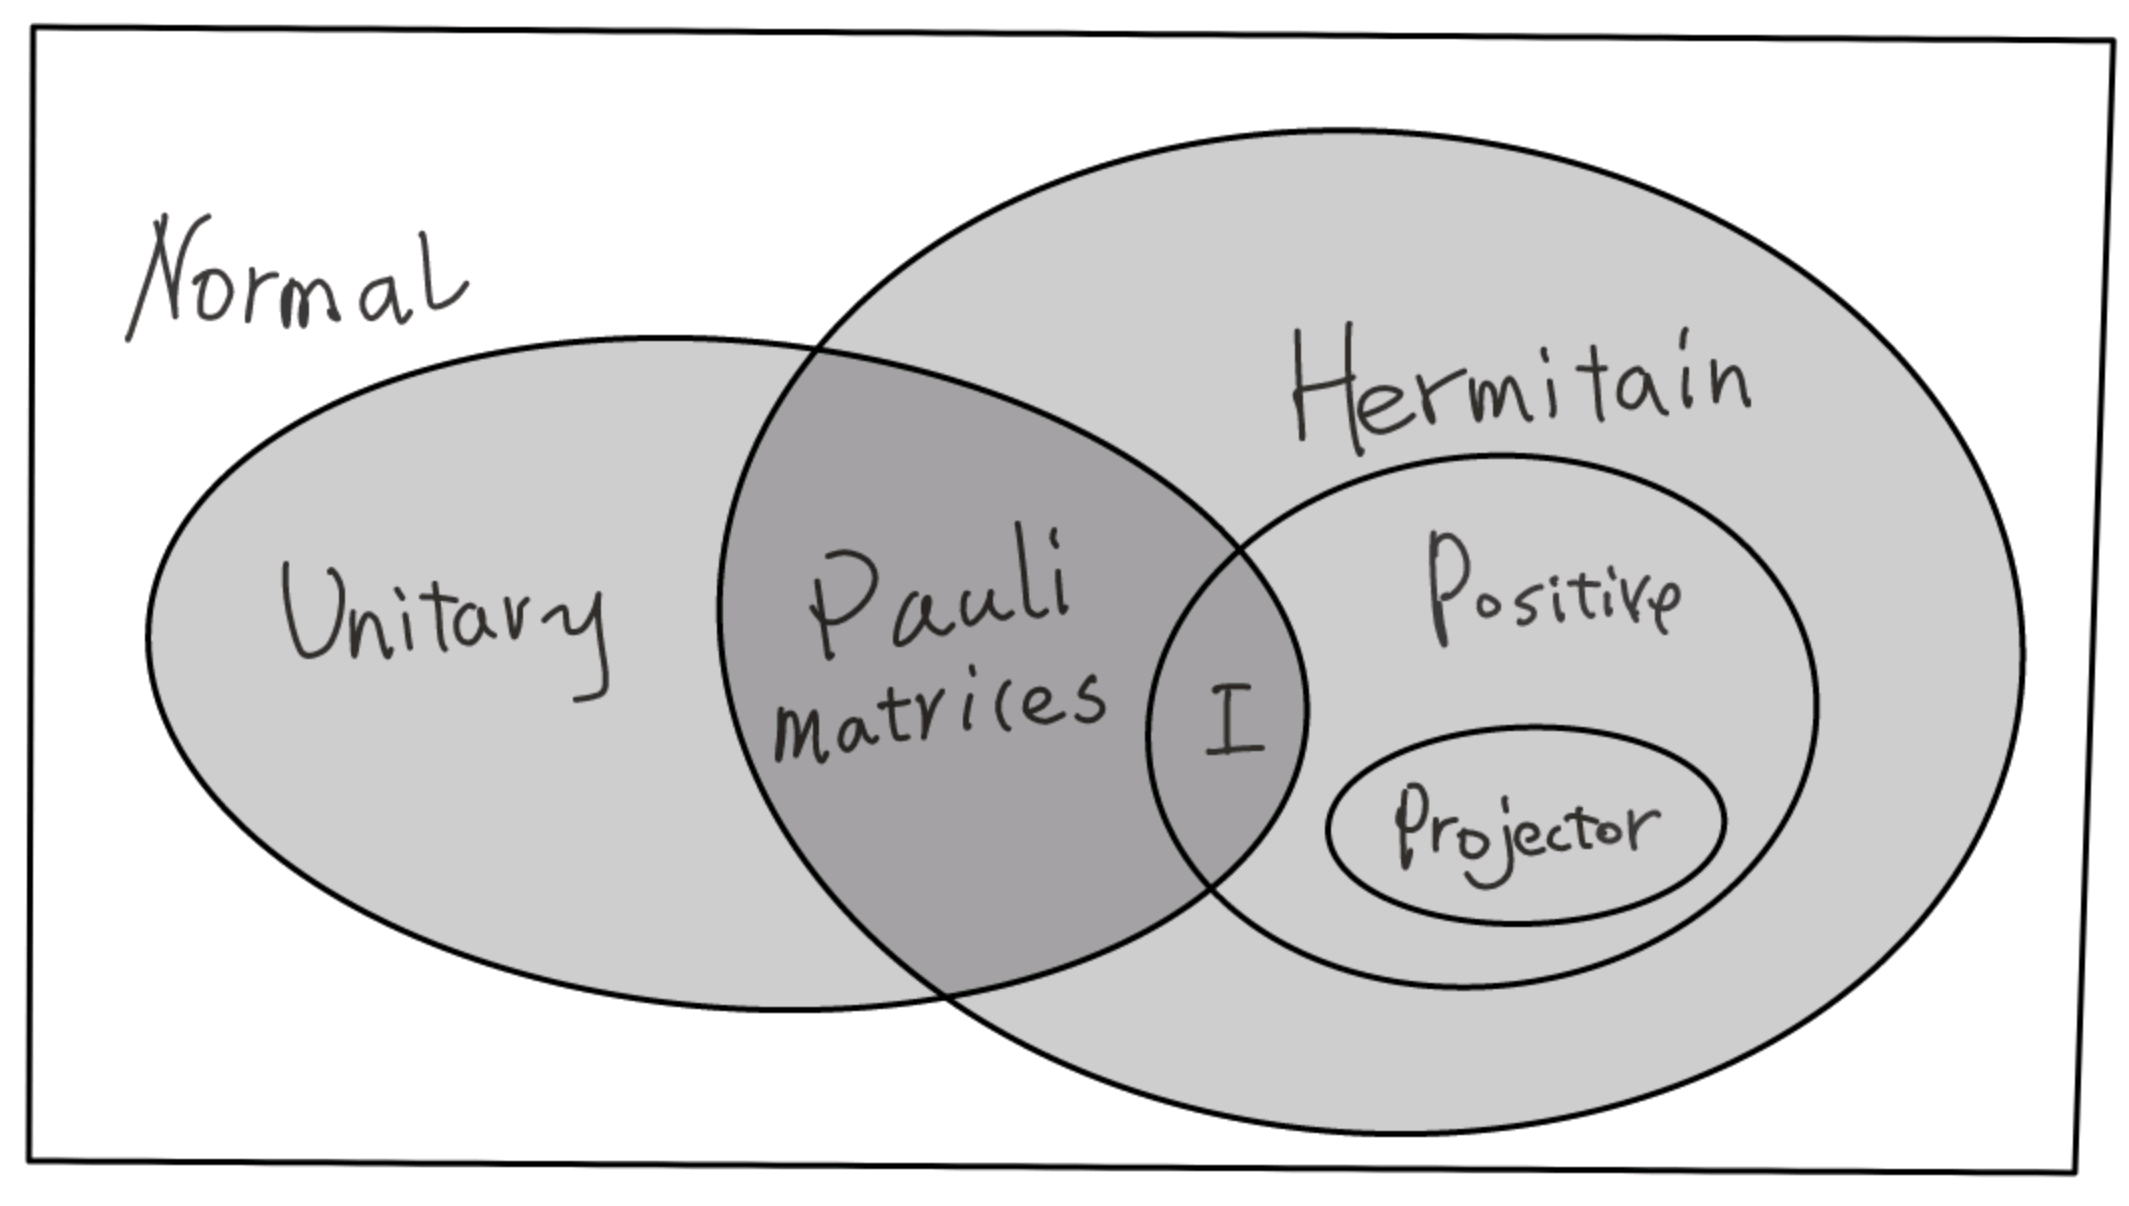
\includegraphics[width=0.75\linewidth]{Images/relations of many operators.png}
    \caption{\textbf{relations of many operators} }
\end{figure}

%   1.1.9 Tensor products
\subsection{Tensor products}
The tensor product is a way of putting vector spaces together to form larger vector spaces. This construction is crucial to understanding the quantum mechanics of multiparticle systems. The following discussion is a little abstract, and may be difficult to follow if you're not already familiar with the tensor product, so feel free to skip ahead now and revisit later when you come to the discussion of tensor products in quantum mechanics.

Suppose $V$ and $W$ are vector spaces of dimension $m$ and $n$ respectively. For convenience we also suppose that $V$ and $W$ are Hilbert spaces. Then $V \otimes W$ (read ' $V$ tensor

Box 2.2: The spectral decomposition - important!

The spectral decomposition is an extremely useful representation theorem for normal operators.

Theorem 2.1: (Spectral decomposition) Any normal operator $M$ on a vector space $V$ is diagonal with respect to some orthonormal basis for $V$. Conversely, any diagonalizable operator is normal.

Proof
The converse is a simple exercise, so we prove merely the forward implication, by induction on the dimension $d$ of $V$. The case $d=1$ is trivial. Let $\lambda$ be an eigenvalue of $M, P$ the projector onto the $\lambda$ eigenspace, and $Q$ the projector onto the orthogonal complement. Then $M=(P+Q) M(P+Q)=P M P+Q M P+$ $P M Q+Q M Q$. Obviously $P M P=\lambda P$. Furthermore, $Q M P=0$, as $M$ takes the subspace $P$ into itself. We claim that $P M Q=0$ also. To see this, let $|v\rangle$ be an element of the subspace $P$. Then $M M^{\dagger}|v\rangle=M^{\dagger} M|v\rangle=\lambda M^{\dagger}|v\rangle$. Thus, $M^{\dagger}|v\rangle$ has eigenvalue $\lambda$ and therefore is an element of the subspace $P$. It follows that $Q M^{\dagger} P=0$. Taking the adjoint of this equation gives $P M Q=0$. Thus $M=P M P+Q M Q$. Next, we prove that $Q M Q$ is normal. To see this, note that $Q M=Q M(P+Q)=Q M Q$, and $Q M^{\dagger}=Q M^{\dagger}(P+Q)=Q M^{\dagger} Q$. Therefore, by the normality of $M$, and the observation that $Q^{2}=Q$,

$$
\begin{aligned}
Q M Q Q M^{\dagger} Q & =Q M Q M^{\dagger} Q \\
& =Q M M^{\dagger} Q \\
& =Q M^{\dagger} M Q \\
& =Q M^{\dagger} Q M Q \\
& =Q M^{\dagger} Q Q M Q
\end{aligned}
$$

so $Q M Q$ is normal. By induction, $Q M Q$ is diagonal with respect to some orthonormal basis for the subspace $Q$, and $P M P$ is already diagonal with respect to some orthonormal basis for $P$. It follows that $M=P M P+Q M Q$ is diagonal with respect to some orthonormal basis for the total vector space.

In terms of the outer product representation, this means that $M$ can be written as $M=\sum_{i} \lambda_{i}|i\rangle\langle i|$, where $\lambda_{i}$ are the eigenvalues of $M,|i\rangle$ is an orthonormal basis for $V$, and each $|i\rangle$ an eigenvector of $M$ with eigenvalue $\lambda_{i}$. In terms of projectors, $M=\sum_{i} \lambda_{i} P_{i}$, where $\lambda_{i}$ are again the eigenvalues of $M$, and $P_{i}$ is the projector onto the $\lambda_{i}$ eigenspace of $M$. These projectors satisfy the completeness relation $\sum_{i} P_{i}=I$, and the orthonormality relation $P_{i} P_{j}=\delta_{i j} P_{i}$.

$W^{\prime}$ ) is an $m n$ dimensional vector space. The elements of $V \otimes W$ are linear combinations of 'tensor products' $|v\rangle \otimes|w\rangle$ of elements $|v\rangle$ of $V$ and $|w\rangle$ of $W$. In particular, if $|i\rangle$ and $|j\rangle$ are orthonormal bases for the spaces $V$ and $W$ then $|i\rangle \otimes|j\rangle$ is a basis for $V \otimes W$. We often use the abbreviated notations $|v\rangle|w\rangle,|v, w\rangle$ or even $|v w\rangle$ for the tensor product\\
$|v\rangle \otimes|w\rangle$. For example, if $V$ is a two-dimensional vector space with basis vectors $|0\rangle$ and $|1\rangle$ then $|0\rangle \otimes|0\rangle+|1\rangle \otimes|1\rangle$ is an element of $V \otimes V$.

By definition the tensor product satisfies the following basic properties:

(1) For an arbitrary scalar $z$ and elements $|v\rangle$ of $V$ and $|w\rangle$ of $W$,

$$
z(|v\rangle \otimes|w\rangle)=(z|v\rangle) \otimes|w\rangle=|v\rangle \otimes(z|w\rangle)
$$

(2) For arbitrary $\left|v_{1}\right\rangle$ and $\left|v_{2}\right\rangle$ in $V$ and $|w\rangle$ in $W$,

$$
\left(\left|v_{1}\right\rangle+\left|v_{2}\right\rangle\right) \otimes|w\rangle=\left|v_{1}\right\rangle \otimes|w\rangle+\left|v_{2}\right\rangle \otimes|w\rangle .
$$

(3) For arbitrary $|v\rangle$ in $V$ and $\left|w_{1}\right\rangle$ and $\left|w_{2}\right\rangle$ in $W$,

$$
|v\rangle \otimes\left(\left|w_{1}\right\rangle+\left|w_{2}\right\rangle\right)=|v\rangle \otimes\left|w_{1}\right\rangle+|v\rangle \otimes\left|w_{2}\right\rangle .
$$

What sorts of linear operators act on the space $V \otimes W$ ? Suppose $|v\rangle$ and $|w\rangle$ are vectors in $V$ and $W$, and $A$ and $B$ are linear operators on $V$ and $W$, respectively. Then we can define a linear operator $A \otimes B$ on $V \otimes W$ by the equation

$$
(A \otimes B)(|v\rangle \otimes|w\rangle) \equiv A|v\rangle \otimes B|w\rangle
$$

The definition of $A \otimes B$ is then extended to all elements of $V \otimes W$ in the natural way to ensure linearity of $A \otimes B$, that is,

$$
(A \otimes B)\left(\sum_{i} a_{i}\left|v_{i}\right\rangle \otimes\left|w_{i}\right\rangle\right) \equiv \sum_{i} a_{i} A\left|v_{i}\right\rangle \otimes B\left|w_{i}\right\rangle .
$$

It can be shown that $A \otimes B$ defined in this way is a well-defined linear operator on $V \otimes W$. This notion of the tensor product of two operators extends in the obvious way to the case where $A: V \rightarrow V^{\prime}$ and $B: W \rightarrow W^{\prime}$ map between different vector spaces. Indeed, an arbitrary linear operator $C$ mapping $V \otimes W$ to $V^{\prime} \otimes W^{\prime}$ can be represented as a linear combination of tensor products of operators mapping $V$ to $V^{\prime}$ and $W$ to $W^{\prime}$,

$$
C=\sum_{i} c_{i} A_{i} \otimes B_{i}
$$

where by definition

$$
\left(\sum_{i} c_{i} A_{i} \otimes B_{i}\right)|v\rangle \otimes|w\rangle \equiv \sum_{i} c_{i} A_{i}|v\rangle \otimes B_{i}|w\rangle .
$$

The inner products on the spaces $V$ and $W$ can be used to define a natural inner product on $V \otimes W$. Define

$$
\left(\sum_{i} a_{i}\left|v_{i}\right\rangle \otimes\left|w_{i}\right\rangle, \sum_{j} b_{j}\left|v_{j}^{\prime}\right\rangle \otimes\left|w_{j}^{\prime}\right\rangle\right) \equiv \sum_{i j} a_{i}^{*} b_{j}\left\langle v_{i} | v_{j}^{\prime}\right\rangle\left\langle w_{i} | w_{j}^{\prime}\right\rangle
$$

It can be shown that the function so defined is a well-defined inner product. From this inner product, the inner product space $V \otimes W$ inherits the other structure we are familiar with, such as notions of an adjoint, unitarity, normality, and Hermiticity.

All this discussion is rather abstract. It can be made much more concrete by moving\\
to a convenient matrix representation known as the Kronecker product. Suppose $A$ is an $m$ by $n$ matrix, and $B$ is a $p$ by $q$ matrix. Then we have the matrix representation:

$$
A \otimes B \equiv \overbrace{\left[\begin{array}{cccc}
A_{11} B & A_{12} B & \ldots & A_{1 n} B \\
A_{21} B & A_{22} B & \ldots & A_{2 n} B \\
\vdots & \vdots & \vdots & \vdots \\
A_{m 1} B & A_{m 2} B & \ldots & A_{m n} B
\end{array}\right]}^{n q} m m p
$$

In this representation terms like $A_{11} B$ denote $p$ by $q$ submatrices whose entries are proportional to $B$, with overall proportionality constant $A_{11}$. For example, the tensor product of the vectors $(1,2)$ and $(2,3)$ is the vector

$$
\left[\begin{array}{l}
1 \\
2
\end{array}\right] \otimes\left[\begin{array}{l}
2 \\
3
\end{array}\right]=\left[\begin{array}{l}
1 \times 2 \\
1 \times 3 \\
2 \times 2 \\
2 \times 3
\end{array}\right]=\left[\begin{array}{l}
2 \\
3 \\
4 \\
6
\end{array}\right]
$$

The tensor product of the Pauli matrices $X$ and $Y$ is

$$
X \otimes Y=\left[\begin{array}{cc}
0 \cdot Y & 1 \cdot Y \\
1 \cdot Y & 0 \cdot Y
\end{array}\right]=\left[\begin{array}{cccc}
0 & 0 & 0 & -i \\
0 & 0 & i & 0 \\
0 & -i & 0 & 0 \\
i & 0 & 0 & 0
\end{array}\right]
$$

Finally, we mention the useful notation $|\psi\rangle^{\otimes k}$, which means $|\psi\rangle$ tensored with itself $k$ times. For example $|\psi\rangle^{\otimes 2}=|\psi\rangle \otimes|\psi\rangle$. An analogous notation is also used for operators on tensor product spaces.

Exercise 2.26: Let $|\psi\rangle=(|0\rangle+|1\rangle) / \sqrt{2}$. Write out $|\psi\rangle^{\otimes 2}$ and $|\psi\rangle^{\otimes 3}$ explicitly, both in terms of tensor products like $|0\rangle|1\rangle$, and using the Kronecker product.

Exercise 2.27: Calculate the matrix representation of the tensor products of the Pauli operators (a) $X$ and $Z$; (b) $I$ and $X$; (c) $X$ and $I$. Is the tensor product commutative?

Exercise 2.28: Show that the transpose, complex conjugation, and adjoint operations distribute over the tensor product,

$$
(A \otimes B)^{*}=A^{*} \otimes B^{*} ;(A \otimes B)^{T}=A^{T} \otimes B^{T} ;(A \otimes B)^{\dagger}=A^{\dagger} \otimes B^{\dagger} .
$$

Exercise 2.29: Show that the tensor product of two unitary operators is unitary.

Exercise 2.30: Show that the tensor product of two Hermitian operators is Hermitian.

Exercise 2.31: Show that the tensor product of two positive operators is positive.

Exercise 2.32: Show that the tensor product of two projectors is a projector.

Exercise 2.33: The Hadamard operator on one qubit may be written as

$$
H=\frac{1}{\sqrt{2}}[(|0\rangle+|1\rangle)\langle 0|+(|0\rangle-|1\rangle)\langle 1|]
$$

Show explicitly that the Hadamard transform on $n$ qubits, $H^{\otimes n}$, may be written as

$$
H^{\otimes n}=\frac{1}{\sqrt{2^{n}}} \sum_{x, y}(-1)^{x \cdot y}|x\rangle\langle y|
$$

Write out an explicit matrix representation for $H^{\otimes 2}$.

%   1.1.10 Operator functions
\subsection{Operator functions}
There are many important functions which can be defined for operators and matrices. Generally speaking, given a function $f$ from the complex numbers to the complex numbers, it is possible to define a corresponding matrix function on normal matrices (or some subclass, such as the Hermitian matrices) by the following construction. Let $A=\sum_{a} a|a\rangle\langle a|$ be a spectral decomposition for a normal operator $A$. Define $f(A) \equiv \sum_{a} f(a)|a\rangle\langle a|$. A little thought shows that $f(A)$ is uniquely defined. This procedure can be used, for example, to define the square root of a positive operator, the logarithm of a positive-definite operator, or the exponential of a normal operator. As an example,

$$
\exp (\theta Z)=\left[\begin{array}{cc}
e^{\theta} & 0 \\
0 & e^{-\theta}
\end{array}\right]
$$

since $Z$ has eigenvectors $|0\rangle$ and $|1\rangle$.

Exercise 2.34: Find the square root and logarithm of the matrix

$$
\left[\begin{array}{ll}
4 & 3 \\
3 & 4
\end{array}\right]
$$

Exercise 2.35: (Exponential of the Pauli matrices) Let $\vec{v}$ be any real, three-dimensional unit vector and $\theta$ a real number. Prove that

$$
\exp (i \theta \vec{v} \cdot \vec{\sigma})=\cos (\theta) I+i \sin (\theta) \vec{v} \cdot \vec{\sigma}
$$

where $\vec{v} \cdot \vec{\sigma} \equiv \sum_{i=1}^{3} v_{i} \sigma_{i}$. This exercise is generalized in Problem 2.1 on page 117.

Another important matrix function is the trace of a matrix. The trace of $A$ is defined to be the sum of its diagonal elements,

$$
\operatorname{tr}(A) \equiv \sum_{i} A_{i i}
$$

The trace is easily seen to be cyclic, $\operatorname{tr}(A B)=\operatorname{tr}(B A)$, and linear, $\operatorname{tr}(A+B)=$ $\operatorname{tr}(A)+\operatorname{tr}(B), \operatorname{tr}(z A)=z \operatorname{tr}(A)$, where $A$ and $B$ are arbitrary matrices, and $z$ is a complex number. Furthermore, from the cyclic property it follows that the trace of a matrix is invariant under the unitary similarity transformation $A \rightarrow U A U^{\dagger}$, as $\operatorname{tr}\left(U A U^{\dagger}\right)=$ $\operatorname{tr}\left(U^{\dagger} U A\right)=\operatorname{tr}(A)$. In light of this result, it makes sense to define the trace of an operator $A$ to be the trace of any matrix representation of $A$. The invariance of the trace under unitary similarity transformations ensures that the trace of an operator is well defined.

As an example of the trace, suppose $|\psi\rangle$ is a unit vector and $A$ is an arbitrary operator. To evaluate $\operatorname{tr}(A|\psi\rangle\langle\psi|)$ use the Gram-Schmidt procedure to extend $|\psi\rangle$ to an\\
orthonormal basis $|i\rangle$ which includes $|\psi\rangle$ as the first element. Then we have

$$
\begin{aligned}
\operatorname{tr}(A|\psi\rangle\langle\psi|) & =\sum_{i}\langle i|A| \psi\rangle\langle\psi | i\rangle \\
& =\langle\psi|A| \psi\rangle
\end{aligned}
$$

This result, that $\operatorname{tr}(A|\psi\rangle\langle\psi|)=\langle\psi|A| \psi\rangle$ is extremely useful in evaluating the trace of an operator.

Exercise 2.36: Show that the Pauli matrices except for $I$ have trace zero.

Exercise 2.37: (Cyclic property of the trace) If $A$ and $B$ are two linear operators show that

$$
\operatorname{tr}(A B)=\operatorname{tr}(B A)
$$

Exercise 2.38: (Linearity of the trace) If $A$ and $B$ are two linear operators, show that

$$
\operatorname{tr}(A+B)=\operatorname{tr}(A)+\operatorname{tr}(B)
$$

and if $z$ is an arbitrary complex number show that

$$
\operatorname{tr}(z A)=z \operatorname{tr}(A)
$$

Exercise 2.39: (The Hilbert-Schmidt inner product on operators) The set $L_{V}$ of linear operators on a Hilbert space $V$ is obviously a vector space - the sum of two linear operators is a linear operator, $z A$ is a linear operator if $A$ is a linear operator and $z$ is a complex number, and there is a zero element 0 . An important additional result is that the vector space $L_{V}$ can be given a natural inner product structure, turning it into a Hilbert space.

(1) Show that the function $(\cdot, \cdot)$ on $L_{V} \times L_{V}$ defined by

$$
(A, B) \equiv \operatorname{tr}\left(A^{\dagger} B\right)
$$

is an inner product function. This inner product is known as the

Hilbert-Schmidt or trace inner product.

(2) If $V$ has $d$ dimensions show that $L_{V}$ has dimension $d^{2}$.

(3) Find an orthonormal basis of Hermitian matrices for the Hilbert space $L_{V}$.

%   1.1.11 The commutator and anti-commutator
\subsection{The commutator and anti-commutator}
The commutator between two operators $A$ and $B$ is defined to be

$$
[A, B] \equiv A B-B A
$$

If $[A, B]=0$, that is, $A B=B A$, then we say $A$ commutes with $B$. Similarly, the anti-commutator of two operators $A$ and $B$ is defined by

$$
\{A, B\} \equiv A B+B A
$$

we say $A$ anti-commutes with $B$ if $\{A, B\}=0$. It turns out that many important properties of pairs of operators can be deduced from their commutator and anti-commutator. Perhaps the most useful relation is the following connection between the commutator and the property of being able to simultaneously diagonalize Hermitian operators $A$ and $B$,\\
that is, write $A=\sum_{i} a_{i}|i\rangle\left\langle i\left|, B=\sum_{i} b_{i}\right| i\right\rangle\langle i|$, where $|i\rangle$ is some common orthonormal set of eigenvectors for $A$ and $B$.

Theorem 2.2: (Simultaneous diagonalization theorem) Suppose $A$ and $B$ are

Hermitian operators. Then $[A, B]=0$ if and only if there exists an orthonormal basis such that both $A$ and $B$ are diagonal with respect to that basis. We say that $A$ and $B$ are simultaneously diagonalizable in this case.

This result connects the commutator of two operators, which is often easy to compute, to the property of being simultaneously diagonalizable, which is a priori rather difficult to determine. As an example, consider that

$$
\begin{aligned}
{[X, Y] } & =\left[\begin{array}{ll}
0 & 1 \\
1 & 0
\end{array}\right]\left[\begin{array}{rr}
0 & -i \\
i & 0
\end{array}\right]-\left[\begin{array}{rr}
0 & -i \\
i & 0
\end{array}\right]\left[\begin{array}{ll}
0 & 1 \\
1 & 0
\end{array}\right] \\
& =2 i\left[\begin{array}{rr}
1 & 0 \\
0 & -1
\end{array}\right] \\
& =2 i Z
\end{aligned}
$$

so $X$ and $Y$ do not commute. You have already shown, in Exercise 2.11, that $X$ and $Y$ do not have common eigenvectors, as we expect from the simultaneous diagonalization theorem.

Proof
You can (and should!) easily verify that if $A$ and $B$ are diagonal in the same orthonormal basis then $[A, B]=0$. To show the converse, let $|a, j\rangle$ be an orthonormal basis for the eigenspace $V_{a}$ of $A$ with eigenvalue $a$; the index $j$ is used to label possible degeneracies. Note that

$$
A B|a, j\rangle=B A|a, j\rangle=a B|a, j\rangle
$$

and therefore $B|a, j\rangle$ is an element of the eigenspace $V_{a}$. Let $P_{a}$ denote the projector onto the space $V_{a}$ and define $B_{a} \equiv P_{a} B P_{a}$. It is easy to see that the restriction of $B_{a}$ to the space $V_{a}$ is Hermitian on $V_{a}$, and therefore has a spectral decomposition in terms of an orthonormal set of eigenvectors which span the space $V_{a}$. Let's call these eigenvectors $|a, b, k\rangle$, where the indices $a$ and $b$ label the eigenvalues of $A$ and $B_{a}$, and $k$ is an extra index to allow for the possibility of a degenerate $B_{a}$. Note that $B|a, b, k\rangle$ is an element of $V_{a}$, so $B|a, b, k\rangle=P_{a} B|a, b, k\rangle$. Moreover we have $P_{a}|a, b, k\rangle=|a, b, k\rangle$, so

$$
B|a, b, k\rangle=P_{a} B P_{a}|a, b, k\rangle=b|a, b, k\rangle .
$$

It follows that $|a, b, k\rangle$ is an eigenvector of $B$ with eigenvalue $b$, and therefore $|a, b, k\rangle$ is an orthonormal set of eigenvectors of both $A$ and $B$, spanning the entire vector space on which $A$ and $B$ are defined. That is, $A$ and $B$ are simultaneously diagonalizable.

Exercise 2.40: (Commutation relations for the Pauli matrices) Verify the commutation relations

$$
[X, Y]=2 i Z ; \quad[Y, Z]=2 i X ; \quad[Z, X]=2 i Y .
$$

There is an elegant way of writing this using $\epsilon_{j k l}$, the antisymmetric tensor on\\
three indices, for which $\epsilon_{j k l}=0$ except for $\epsilon_{123}=\epsilon_{231}=\epsilon_{312}=1$, and $\epsilon_{321}=\epsilon_{213}=\epsilon_{132}=-1:$

$$
\left[\sigma_{j}, \sigma_{k}\right]=2 i \sum_{l=1}^{3} \epsilon_{j k l} \sigma_{l}
$$

Exercise 2.41: (Anti-commutation relations for the Pauli matrices) Verify the anti-commutation relations

$$
\left\{\sigma_{i}, \sigma_{j}\right\}=0
$$

where $i \neq j$ are both chosen from the set $1,2,3$. Also verify that $(i=0,1,2,3)$

$$
\sigma_{i}^{2}=I
$$

Exercise 2.42: Verify that

$$
A B=\frac{[A, B]+\{A, B\}}{2}
$$

Exercise 2.43: Show that for $j, k=1,2,3$,

$$
\sigma_{j} \sigma_{k}=\delta_{j k} I+i \sum_{l=1}^{3} \epsilon_{j k l} \sigma_{l}
$$

Exercise 2.44: Suppose $[A, B]=0,\{A, B\}=0$, and $A$ is invertible. Show that $B$ must be 0 .

Exercise 2.45: Show that $[A, B]^{\dagger}=\left[B^{\dagger}, A^{\dagger}\right]$.

Exercise 2.46: Show that $[A, B]=-[B, A]$.

Exercise 2.47: Suppose $A$ and $B$ are Hermitian. Show that $i[A, B]$ is Hermitian.

%   1.1.12 The polar and singular value decomposition
\subsection{The polar and singular value decomposition}
The polar and singular value decompositions are useful ways of breaking linear operators up into simpler parts. In particular, these decompositions allow us to break general linear operators up into products of unitary operators and positive operators. While we don't understand the structure of general linear operators terribly well, we do understand unitary operators and positive operators in quite some detail. The polar and singular value decompositions allow us to apply this understanding to better understand general linear operators.

Theorem 2.3: (Polar decomposition) Let $A$ be a linear operator on a vector space $V$. Then there exists unitary $U$ and positive operators $J$ and $K$ such that

$$
A=U J=K U
$$

where the unique positive operators $J$ and $K$ satisfying these equations are defined by $J \equiv \sqrt{A^{\dagger} A}$ and $K \equiv \sqrt{A A^{\dagger}}$. Moreover, if $A$ is invertible then $U$ is unique.

We call the expression $A=U J$ the left polar decomposition of $A$, and $A=K U$ the right polar decomposition of $A$. Most often, we'll omit the 'right' or 'left' nomenclature, and use the term 'polar decomposition' for both expressions, with context indicating which is meant.

Proof

$J \equiv \sqrt{A^{\dagger} A}$ is a positive operator, so it can be given a spectral decomposition, $J=$ $\sum_{i} \lambda_{i}|i\rangle\langle i|\left(\lambda_{i} \geq 0\right)$. Define $\left|\psi_{i}\right\rangle \equiv A|i\rangle$. From the definition, we see that $\left\langle\psi_{i} | \psi_{i}\right\rangle=\lambda_{i}^{2}$. Consider for now only those $i$ for which $\lambda_{i} \neq 0$. For those $i$ define $\left|e_{i}\right\rangle \equiv\left|\psi_{i}\right\rangle / \lambda_{i}$, so the $\left|e_{i}\right\rangle$ are normalized. Moreover, they are orthogonal, since if $i \neq j$ then $\left\langle e_{i} | e_{j}\right\rangle=$ $\left\langle i\left|A^{\dagger} A\right| j\right\rangle / \lambda_{i} \lambda_{j}=\left\langle i\left|J^{2}\right| j\right\rangle / \lambda_{i} \lambda_{j}=0$

We have been considering $i$ such that $\lambda_{i} \neq 0$. Now use the Gram-Schmidt procedure to extend the orthonormal set $\left|e_{i}\right\rangle$ so it forms an orthonormal basis, which we also label $\left|e_{i}\right\rangle$. Define a unitary operator $U \equiv \sum_{i}\left|e_{i}\right\rangle\langle i|$. When $\lambda_{i} \neq 0$ we have $U J|i\rangle=\lambda_{i}\left|e_{i}\right\rangle=$ $\left|\psi_{i}\right\rangle=A|i\rangle$. When $\lambda_{i}=0$ we have $U J|i\rangle=0=\left|\psi_{i}\right\rangle$. We have proved that the action of $A$ and $U J$ agree on the basis $|i\rangle$, and thus that $A=U J$.

$J$ is unique, since multiplying $A=U J$ on the left by the adjoint equation $A^{\dagger}=J U^{\dagger}$ gives $J^{2}=A^{\dagger} A$, from which we see that $J=\sqrt{A^{\dagger} A}$, uniquely. A little thought shows that if $A$ is invertible, then so is $J$, so $U$ is uniquely determined by the equation $U=A J^{-1}$. The proof of the right polar decomposition follows, since $A=U J=U J U^{\dagger} U=K U$, where $K \equiv U J U^{\dagger}$ is a positive operator. Since $A A^{\dagger}=K U U^{\dagger} K=K^{2}$ we must have $K=\sqrt{A A^{\dagger}}$, as claimed.

The singular value decomposition combines the polar decomposition and the spectral theorem.

Corollary 2.4: (Singular value decomposition) Let $A$ be a square matrix. Then there exist unitary matrices $U$ and $V$, and a diagonal matrix $D$ with non-negative entries such that

$$
A=U D V
$$

The diagonal elements of $D$ are called the singular values of $A$.

Proof

By the polar decomposition, $A=S J$, for unitary $S$, and positive $J$. By the spectral theorem, $J=T D T^{\dagger}$, for unitary $T$ and diagonal $D$ with non-negative entries. Setting $U \equiv S T$ and $V \equiv T^{\dagger}$ completes the proof.

Exercise 2.48: What is the polar decomposition of a positive matrix P? Of a unitary matrix $U$ ? Of a Hermitian matrix, $H$ ?

Exercise 2.49: Express the polar decomposition of a normal matrix in the outer product representation.

Exercise 2.50: Find the left and right polar decompositions of the matrix

$$
\left[\begin{array}{ll}
1 & 0 \\
1 & 1
\end{array}\right]
$$


\subsection{Partial trace}
% 主要参考wiki
% \href{https://en.wikipedia.org/wiki/Partial_trace}{Partial trace - Wikipedia}

In linear algebra and functional analysis, the partial trace is a generalization of the trace. 
Whereas the trace is a scalar valued function on operators, the partial trace is an operator-valued function.

Suppose $V, W$ are finite-dimensional vector spaces over a field, with dimensions $m$ and $n$, respectively. 
For any vector space $A$, let $L(A)$ denote the space of linear operators on $A$.

\begin{definition}[partial trace I]\label{defn:partial-trace-1}
The \textbf{partial trace over $W$} is an operator-valued function written as
$$
\operatorname{Tr}_W: \mathrm{L}(V \otimes W) \rightarrow \mathrm{L}(V),
$$
where $\otimes$ denotes the tensor product. It is defined as follows: Let $e_1, \ldots, e_m$, and $f_1, \ldots, f_n$, be bases for $V$ and $W$ respectively; then $T \in \mathrm{L}(V \otimes W)$ has a matrix representation
$$
a_{k \ell, i j}, \quad 1 \leq k, i \leq m, \quad 1 \leq \ell, j \leq n
$$
relative to the basis $e_k \otimes f_{\ell}$ of $V \otimes W$. Now fix indices $k, i$ in the range $1, \ldots, m$, consider the sum
$$
b_{k, i}=\sum_{j=1}^n a_{k j, i j}
$$
This gives a matrix $b_{k, i}$. The associated linear operator (of matrix $b_{k, i}$) on \textit{V} is independent of the choice of bases and is by definition the partial trace.
\end{definition}

Among physicists, this is often called \textbf{"tracing out" or "tracing over" $W$} to leave only an operator on $V$ in the context where $W$ and $V$ are Hilbert spaces associated with quantum systems (see below).

The partial trace operator can be defined invariantly (that is, without reference to a basis) as follows.

\begin{definition}[partial trace II]
The \textbf{partial trace over $W$} is the unique linear map
$$
\operatorname{Tr}_W: \mathrm{L}(V \otimes W) \rightarrow \mathrm{L}(V)
$$
such that
\begin{equation}\label{eq:partial-trace-defn}
    \operatorname{Tr}_W(R \otimes S)=\operatorname{Tr}(S) R, \quad \forall R \in \mathrm{L}(V) \quad \forall S \in \mathrm{L}(W),
\end{equation}
where $\operatorname{Tr}(\cdot)$ is the usual trace of a linear operator.
\end{definition}

\begin{proof} % lai's proof
Definition \ref{defn:partial-trace-1} showed such linear map exists.
To see that the conditions (\ref{eq:partial-trace-defn}) determine the partial trace uniquely:
\begin{itemize}
  \item let $v_1, \ldots, v_m$ form an orthonormal basis for $V$ and let $w_1, \ldots, w_n$ form an orthonormal for $W$;
  \item let $E_{i j}: V \rightarrow V$ be the map that sends $v_i$ to $v_j$ (and all other basis elements to zero), then the maps $E_{i j}$ form a basis for $\mathrm{L}(V)$.
  \item let $F_{k l}: W \rightarrow W$ be the map that sends $w_k$ to $w_l$ (and all other basis elements to zero), then the maps $F_{k l}$ form a basis for $\mathrm{L}(W)$.
  \item we have $\operatorname{Tr}(E_{ij})=\operatorname{Tr}(F_{kl})=1.$
  \item since the vectors $v_i \otimes w_k$ form a basis for $V \otimes W$, the maps $E_{i j} \otimes F_{k l}$ form a basis for $\mathrm{L}(V \otimes W)$.
  \item for given \textit{any} partial trace $\operatorname{Tr}_W$, we always have that
\end{itemize}
$$
\operatorname{Tr}_W(E_{i j} \otimes F_{k l})=\operatorname{Tr}(F_{k l}) E_{i j} = E_{i j}.
$$
\end{proof}

From this abstract definition, the following properties follow:

\begin{proposition}
$$
\begin{aligned}
& \operatorname{Tr}_W\left(T\left(I_V \otimes S\right)\right)=\operatorname{Tr}_W\left(\left(I_V \otimes S\right) T\right) ,\quad \forall S \in \mathrm{L}(W) \quad \forall T \in \mathrm{L}(V \otimes W).
\end{aligned}
$$
\end{proposition}

\begin{proof}
    my proof is done on
\end{proof}

The partial trace can be viewed as a quantum operation.

Consider a quantum mechanical system whose state space is the tensor product $H_A \otimes H_B$ of Hilbert spaces. A mixed state is described by a density matrix $\rho$, that is a non-negative trace-class operator of trace 1 on the tensor product $H_A \otimes H_B$. The partial trace of $\rho$ with respect to the system $B$, denoted by $\rho^A$, is called the reduced state of $\rho$ on system $A$. In symbols,
$$
\rho^A=\operatorname{Tr}_B \rho
$$

To show that this is indeed a sensible way to assign a state on the $A$ subsystem to $\rho$, we offer the following justification. 

Let $M$ be an observable on the subsystem $A$, then the corresponding observable on the composite system is $M \otimes I$. However one chooses to define a reduced state $\rho^A$, there should be consistency of measurement statistics. The expectation value of $M$ after the subsystem $A$ is prepared in $\rho^A$ and that of $M \otimes I$ when the composite system is prepared in $\rho$ should be the same, i.e. the following equality should hold:
$$
\operatorname{Tr}\left(M \cdot \rho^A\right)=\operatorname{Tr}(M \otimes I \cdot \rho) .
$$
We see that this is satisfied if $\rho^A$ is as defined above via the partial trace. Furthermore, such operation is unique.

\begin{proof}
    my proof is done on
\end{proof}

\subsection{Discrete Fourier transform}

\href{https://en.wikipedia.org/wiki/Discrete_Fourier_transform}{Discrete Fourier transform - Wikipedia}

\begin{definition}
The \textbf{discrete Fourier transform (DFT)} transforms a sequence of $N$ complex numbers $\left\{\mathbf{x}_n\right\}:=x_0, x_1, \ldots, x_{N-1}$ into another sequence of complex numbers, $\left\{\mathbf{X}_k\right\}:=X_0, X_1, \ldots, X_{N-1}$, which is defined by:
$$
X_k=\sum_{n=0}^{N-1} x_n \cdot e^{-i 2 \pi \frac{k}{N} n}
$$
The transform is sometimes denoted by the symbol $\mathcal{F}$, as in $\mathbf{X}=\mathcal{F}\{\mathbf{x}\}$ or $\mathcal{F}(\mathbf{x})$ or $\mathcal{F} \mathbf{x}$.
\end{definition}

The inverse transform is given by:
$$
x_n=\frac{1}{N} \sum_{k=0}^{N-1} X_k \cdot e^{i 2 \pi \frac{k}{N} n}
$$

\begin{example}
    This example demonstrates how to apply the DFT to a sequence of length $N=4$ and the input vector
$$
\mathbf{x}=\left(\begin{array}{l}
x_0 \\
x_1 \\
x_2 \\
x_3
\end{array}\right)=\left(\begin{array}{c}
1 \\
2-i \\
-i \\
-1+2 i
\end{array}\right) .
$$
Calculating the DFT of $\mathbf{x}$ using Eq. 1
$$
\begin{aligned}
& X_0=e^{-i 2 \pi v \cdot u / 4} \cdot 1+e^{-\imath 2 \pi v \cdot 1 / 4} \cdot(2-i)+e^{-\imath 2 \pi v \cdot 2 / 4} \cdot(-i)+e^{-\imath 2 \pi v \cdot 3 / 4} \cdot(-1+2 i)=2 \\
& X_1=e^{-i 2 \pi 1 \cdot 0 / 4} \cdot 1+e^{-i 2 \pi 1 \cdot 1 / 4} \cdot(2-i)+e^{-i 2 \pi 1 \cdot 2 / 4} \cdot(-i)+e^{-i 2 \pi 1 \cdot 3 / 4} \cdot(-1+2 i)=-2-2 i \\
& X_2=e^{-i 2 \pi 2 \cdot 0 / 4} \cdot 1+e^{-i 2 \pi 2 \cdot 1 / 4} \cdot(2-i)+e^{-i 2 \pi 2 \cdot 2 / 4} \cdot(-i)+e^{-i 2 \pi 2 \cdot 3 / 4} \cdot(-1+2 i)=-2 i \\
& X_3=e^{-i 2 \pi 3 \cdot 0 / 4} \cdot 1+e^{-i 2 \pi 3 \cdot 1 / 4} \cdot(2-i)+e^{-i 2 \pi 3 \cdot 2 / 4} \cdot(-i)+e^{-i 2 \pi 3 \cdot 3 / 4} \cdot(-1+2 i)=4+4 i
\end{aligned}
$$
results in
$$
\mathbf{X}=\left(\begin{array}{c}
X_0 \\
X_1 \\
X_2 \\
X_3
\end{array}\right)=\left(\begin{array}{c}
2 \\
-2-2 i \\
-2 i \\
4+4 i
\end{array}\right)
$$
\end{example}



\paragraph{Linearity}

The DFT is a linear transform, i.e. if $\mathcal{F}\left(\left\{x_n\right\}\right)_k=X_k$ and $\mathcal{F}\left(\left\{y_n\right\}\right)_k=Y_k$, then for any complex numbers $a, b$:
$$
\mathcal{F}\left(\left\{a x_n+b y_n\right\}\right)_k=a X_k+b Y_k.
$$

\paragraph{Orthogonality}
The vectors $u_k=\left[\left.e^{\frac{i 2 \pi}{N} k n} \right\rvert\, n=0,1, \ldots, N-1\right]^{\top}$ form an orthogonal basis over the set of $N$-dimensional complex vectors:
$$
u_k^{\top} u_{k^{\prime}}^*=\sum_{n=0}^{N-1}\left(e^{\frac{i 2 \pi}{N} k n}\right)\left(e^{\frac{i 2 \pi}{N}\left(-k^{\prime}\right) n}\right)=\sum_{n=0}^{N-1} e^{\frac{i 2 \pi}{N}\left(k-k^{\prime}\right) n}=N \delta_{k k^{\prime}}.
$$
where $\delta_{k k^{\prime}}$ is the Kronecker delta. (In the last step, the summation is trivial if $k=k^{\prime}$, where it is $1+1+\ldots=N$ and otherwise is a geometric series that can be explicitly summed to obtain zero.) This orthogonality condition can be used to derive the formula for the IDFT from the definition of the DFT, and is equivalent to the unitarity property below.




%----------------------------------------------------------------------------------------
%	PART II
%----------------------------------------------------------------------------------------

\part{Notes of Papers}

% \chapter{Variational Quantum Algorithms}

\chapter{grange2023introduction}

"An introduction to variational quantum algorithms for combinatorial optimization problems" \cite{grange2023introduction}

\vspace{10pt}

Variational Quantum Algorithms are heuristic algorithms that alternate between a quantum circuit and a classical optimizer. They tackle optimization problems of the form
\begin{equation}
    \min _{x \in\{0,1\}^n} f(x), \tag{1}
\end{equation}
where $f$ is any function defined on $\{0,1\}^n$. 


\section{Basics of quantum computing for combinatorial optimization}

\subsection{2.1 Quantum bits \& 2.2 Quantum gates}

Definition 3 (Canonical basis) The canonical basis of an $n$-qubit state is the set
$$
\mathcal{C B}_{n}=\left(\bigotimes_{k=1}^{n}\left|i^{(k)}\right\rangle,\left(i^{(1)}, \ldots, i^{(n)}\right) \in\{0,1\}^{n}\right)
$$
where $i^{(k)}$ represents the state of the $k$-th qubit and $\otimes$ is the tensor product defined in Appendix A. The canonical basis is the set of all possible combinations of tensor products of $n$ one-qubit basis states, $|0\rangle$ and $|1\rangle$. Thus, in the matrix representation, each canonical basis state is a column vector of $2^{n}$ components with one component equal to 1 and the rest equal to 0 . It directly results that the size of the canonical basis of an $n$-qubit state is $2^{n}$. For more readability, we omit to write the tensor product between qubits, i.e.,
$$
\mathcal{C B}_{n}=\left(|i\rangle, i \in\{0,1\}^{n}\right)
$$
\begin{remark}
    \begin{itemize}
        \item $\left|\Phi^{+}\right\rangle=\frac{|00\rangle+|11\rangle}{\sqrt{2}}$
        \item reversible %可逆的,相当于数学用语inverse, invertible
        \item circuit representation of a quantum gate
        \item each horizontal line is associated with a qubit
    \end{itemize}
\end{remark}

\subsection{2.3 Quantum circuits}

In the circuit representation, qubits are numbered \textit{in ascending order from top to bottom} which is important for the tensor product circuit representation that follows. % 注意从电路图上看,composition的顺序是从左边到右边,而tensor的顺序是从上边到下边。这两类操作都是不可交换的操作,所以顺序很重要。

\subsubsection{Manipulate quantum gates to build other quantum gates}

We can manipulate quantum gates to build other quantum gates in two different ways. 
\begin{enumerate}
    \item The first one is the composition. The composition of gates only operates between gates acting on the same qubits. 
\begin{figure}
    \centering
    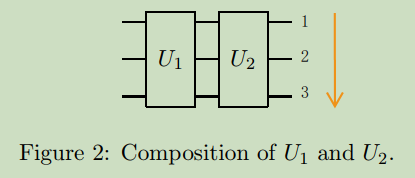
\includegraphics[width=0.5\linewidth]{Images/grange2023-1.png}
\end{figure}
    \item The other one is the tensor product. The tensor product of gates can operates between gates acting on different qubits. Suppose $U_{1} \in \mathcal{M}_{2^{k}}(\mathbb{C})$ applies on the first $k$ qubits and $U_{2} \in \mathcal{M}_{2^{\prime}}(\mathbb{C})$ applies on the $k^{\prime}$ following ones. Their tensor product is the application of $U_{1}$ and $U_{2}$ on respective qubits in parallel. The matrix representation of this tensor product is $U_{1} \otimes U_{2}$ . 
\begin{figure}
    \centering
    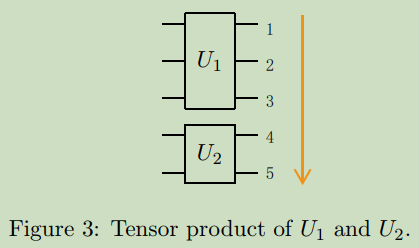
\includegraphics[width=0.5\linewidth]{Images/grange2023-2.png}
\end{figure}
    \item One readily verifies that both composition and tensor product transform unitary matrices into a resulting unitary matrix.
\end{enumerate}

Notice that when we apply a quantum gate on $k$ qubits of an $n$-qubit system, it supposes that we apply identity gate $I$ on the qubits not concerned. 

\begin{example}
For instance, let us consider a 3-qubit system on which we apply $U \in \mathcal{M}_{2}(\mathbb{C})$ on qubit number 2. The matrix representation of the resulting 3 -qubit gate is $I \otimes U \otimes I$, and its circuit representation is illustrated on Fig.4, where the application of $I$ is usually replaced by a simple wire.
    \begin{figure}
    \centering
    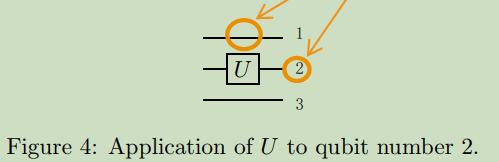
\includegraphics[width=0.5\linewidth]{Images/grange2023-3.png}
\end{figure}
\end{example}

\subsubsection{What is a quantum algorithm?}

Throughout, we consider that \textit{a quantum algorithm is a quantum circuit acting on $n$ qubits, that is, a sequence of quantum gates' compositions and/or tensor products. } % 概括得挺好

These quantum gates can be $k$-qubit gates, for $k \in[n]$. % k是小于等于n的整数。相对于很大n,当k足够小时,k-qubit gates 就可以称之为 small gates。

However, quantum gates involving many qubits are typically not implementable natively on quantum computers and need to be decomposed into smaller and simpler gates. This set of small gates can be considered as the quantum counterpart of the elementary logic gates used in classical circuit computing to assess \textit{the circuit complexity} of a classical algorithm. % 也就是说电路的复杂度可以由构成其的基础gates的个数来做衡量,这一想法是来自于经典电路的。

Thus, an $n$-qubit quantum algorithm is described by a unitary matrix in $\mathcal{M}_{2^{n}}(\mathbb{C})$, and we decompose it as a sequence of universal gates to obtain the \textit{complexity of the quantum algorithm}. % 也就是说量子电路的复杂度可以由构成其的基础量子gates的个数来做衡量

\subsubsection{Universal gates }

\begin{definition}
    Definition 11 (Set of universal gates) A set of quantum gates PU is universal if we can decompose any $n$-qubit quantum gate through a circuit composed solely of the gates in PU.
\end{definition}

\begin{remark}
\begin{itemize}
    \item In definition above, we implicitly allow PU to be a set of infinite elements (countable or uncountable). Of course, we want PU to be small as soon as possible.
    \item In definition above, the word "composed" contains both the composition operations and tensor product operations.
    \item Note that this "decompose" is exact decomposition, and there no error.
\end{itemize}
\end{remark}

Fortunately, there exist different universal sets of quantum gates. We introduce below such a set formed of four types of gates. 

\begin{example}[Some important small gates]
First, we consider the three following families of one-qubit gates, each of which is parametrized by a real number $\theta \in \mathbb{R}$ :
\begin{align*}
& R_{X}(\theta)=\left(\begin{array}{cc}
\cos \frac{\theta}{2} & -i \sin \frac{\theta}{2} \\
-i \sin \frac{\theta}{2} & \cos \frac{\theta}{2}
\end{array}\right)  \tag{5}\\
& R_{Y}(\theta)=\left(\begin{array}{cc}
\cos \frac{\theta}{2} & -\sin \frac{\theta}{2} \\
\sin \frac{\theta}{2} & \cos \frac{\theta}{2}
\end{array}\right)  \tag{6}\\
& R_{Z}(\theta)=\left(\begin{array}{cc}
e^{-i \frac{\theta}{2}} & 0 \\
0 & e^{i \frac{\theta}{2}}
\end{array}\right) \tag{7}
\end{align*}
 Second, we consider the two-qubit gate CX (or, CNOT, Controlled Not, Controlled X gate):
\[
C X=\left(\begin{array}{llll}
1 & 0 & 0 & 0  \tag{8}\\
0 & 1 & 0 & 0 \\
0 & 0 & 0 & 1 \\
0 & 0 & 1 & 0
\end{array}\right)
\]
In other words, we can define $C X$ on the canonical basis as
$$
C X|a, b\rangle=|a, b \oplus a\rangle
$$
for $a, b \in\{0,1\}$, where $\oplus$ is the addition modulo 2 .
\end{example}

\begin{remark}%Notation on gates indexes
Henceforth, we use the notation $R_{X, i}$ for the application of $R_{X}$ on qubit $i$ (and the application of identity matrix on the remaining qubits). We do the same with $R_{Y, i}$ and $R_{Z, i}$. 
% 这一中比较偷懒的写法:$R_{X, i}$,可以用来表示一个非常大的gates,但其中只有第i个qubit是受到非平凡的$R_{X}$的操作。这类写法在其他文献中也经常使用。

We note $C X_{i, j}$ the application of $C X$ gate to qubits $i$ and $j: X$ is applied to qubit $j$ if and only if qubit $i$ is in state $|1\rangle$.
% 明确标记控制位和操作位也是CX门常见写法。但有时不同文献会有细微差别,要注意别混淆。
\end{remark}

\begin{theorem}[Universal gates \cite{nielsen2010quantum}]
Theorem 13
\begin{itemize}
    \item The set of all one-qubit gates and the $C X$ gate is universal.
    \item Any one-qubit gate is the composition of rotation gates (5)-(7).
    \item Thus, the set 
$$
P U=\left\{R_{X}(\alpha), R_{Y}(\beta), R_{Z}(\gamma), C X: \alpha, \beta, \gamma \in \mathbb{R}\right\}
$$
is also universal.
\end{itemize}
\end{theorem}

In comparison, the sets of gates $\{N A N D\},\{N O R\},\{N O T, A N D\}$ and $\{N O T, O R\}$ are universal for classical computation. \todo{Need proof.} Indeed, we can compute any arbitrary classical function with them. % 这一部分知识是传统计算科学里出现的证明,未来有时间好好研究一下。

In view of the above, we typically consider that the quantum counterpart of the classical number of elementary operations is the number of universal gates used to decompose the circuit. Of course, this decomposition depends on the set of universal gates $P U$ considered, but the number of gates required is the same with any set, modulo a multiplicative constant. 

% Thereafter, we only consider the set $P U$ defined in Theorem 13. This choice is motivated by the algorithms we study in this paper, as it will be convenient to express them with this set. 

Furthermore, if we consider the family of circuits $\left(\mathcal{C}_{n}\right)_{n \in \mathbb{N}}$ where $\mathcal{C}_{n}$ is a circuit on $n$ qubits and is decomposed on $\mathcal{O}(\operatorname{poly}(n))$ universal quantum gates, then this family is said to be \textit{efficient}.

\subsection{2.4 Non-classical behaviors} % 确实,前面几节没有让人感觉奇怪的设定。作者把量子特有的设定放在一起,以区别经典行为。这一思路值得借鉴。

The quantum algorithms rely on three characteristics of quantum states with no classical equivalent: measurement, superposition, and entanglement.

\subsubsection{Measurement} %该论文的测量介绍,把很艰难晦涩的测量,用短短的语言就清晰地刻画了。很值得学习。他不涉及各种客观测量,投影算子,POVM等复杂概念。

We need to measure a quantum state $|\psi\rangle$ to get information from it; otherwise, no information is accessible.
Moreover, it only extracts partial information from the quantum state at once measurement: the single measurement output of  $|\psi\rangle$ is a bitstring\footnote{$n$-bitstring is the element of $\{0,1\}^{n}$}.

\begin{definition}
    Definition 14 (Measurement) In the gate-based quantum model, the measurement $\mathcal{M}$ of an $n$-qubit state $|\psi\rangle=\sum_{i \in\{0,1\}^{n}} \psi_{i}|i\rangle$ outputs the $n$-bitstring $i$ with probability $\left|\psi_{i}\right|^{2}$. After having been measured, state $|\psi\rangle$ no longer exists: it has been replaced by the state $|i\rangle$.
\end{definition}

\begin{example}
    For example, measuring qubit $|q\rangle=q_{0}|0\rangle+q_{1}|1\rangle$ outputs 0 with probability $\left|q_{0}\right|^{2}$ and 1 with probability $\left|q_{1}\right|^{2}$, and changes the state $|q\rangle$ to $|0\rangle$ and $|1\rangle$, respectively.  % 这个例子值得玩味的点是,我们测量得到的结果outcome是label(用bitstring表示),而原量子态坍缩成对应的label的basis state。所以,不应该说,测量得到的结果就是basis state自身。
\end{example}

Some points:
\begin{itemize}
    \item A measurement appears as a loss of information. Indeed, we describe an $n$-qubit state by $2^{n}$ normalized complex coefficients, but we only extract an $n$-bitstring after measuring it. 
    \item The perfect knowledge of the \textit{probabilities representing a given quantum state $|\psi\rangle$}, namely, the square module of each of its coordinates $\left(\left|\psi_{i}\right|^{2}\right)_{i \in\{0,1\}^{n}} \in[0,1]^{2^{n}}$, can be obtained \textit{only if we measure $|\psi\rangle$ an infinite number of times.} Notice that it requires resetting state $|\psi\rangle$ after each measurement.
    \item Note that we never get the exact complex numbers $\psi_{i}$, instead of, their squared module $\left|\psi_{i}\right|^{2}$ at most.
    \item Different qubit state might have the same probabilities representing.
\end{itemize}

In reality we are limited to approximating a given quantum state through sampling. In particular, if $|\psi\rangle$ is the result of an algorithm, this means we have to repeat the same algorithm for every measurement of $|\psi\rangle$ we wish to perform.

\subsubsection{Superposition}

Definition 16 (Superposition) A quantum state $|\psi\rangle$ is said in superposition if $|\psi\rangle=$ $\sum_{i \in\{0,1\}^{n}} \psi_{i}|i\rangle$ where there are \textit{at least two terms }with non-zero coefficients in the sum. Equivalently, a quantum state that is not a basis state is in superposition.

\begin{remark}
    \begin{itemize}
        \item A quantum state is in superposition. = A quantum state is superposed. 
        \item A quantum stated superposed is $\dots$
    \end{itemize}
\end{remark}

The Hadamard gate $H=\frac{1}{\sqrt{2}}\left(\begin{array}{cc}1 & 1 \\ 1 & -1\end{array}\right)$ is essential in quantum computing because it creates superposition starting from a basis state. We obtain the state $|+\rangle$, respectively $|-\rangle$, by applying $H$ on $|0\rangle$, respectively $|1\rangle:$
$$
\begin{aligned}
& H|0\rangle=\frac{|0\rangle+|1\rangle}{\sqrt{2}}=:|+\rangle \\
& H|1\rangle=\frac{|0\rangle-|1\rangle}{\sqrt{2}}=:|-\rangle
\end{aligned}
$$
The two states $|+\rangle$ and $|-\rangle$ are in uniform superposition because both have the same probability of being measured as 0 or 1. 

\begin{definition}
    In general, an $n$-qubit state is in \textbf{uniformly superposition} if it is equal to 
$$
\frac{1}{\sqrt{2^{n}}} \sum_{j \in\{0,1\}^{n}} e^{i \alpha_{j}}|j\rangle,
$$
with $\alpha_{j} \in\left[0,2 \pi\left[, \forall j \in\{0,1\}^{n}\right.\right.$. % 注意,uniform的含义不是非要各个系数自身相等,而是他们的modulus相等。下面的$|+\rangle^{\otimes n}$ 提供一种各个系数自身相等的特殊情况。
In what follows, we shall often use the following uniformly superposed $n$-qubit state 
$$
|+\rangle^{\otimes n}=\frac{1}{\sqrt{2^{n}}} \sum_{i \in\{0,1\}^{n}}|i\rangle.
$$
\end{definition}

\begin{remark} 
Some points in definition above:
    \begin{itemize}
        \item $[0,2 \pi[$ equals $[0,2 \pi)$.
        \item sometimes, we need carefully distinguish "index $i$ " with "pure imaginary number i". 
    \end{itemize}
\end{remark}

When applying the tensor product of $n$ Hadamard gates, each applied to a qubit initially in state $|0\rangle$, specifically
\begin{equation*}
H^{\otimes n}|0\rangle^{\otimes n}=\bigotimes_{i=1}^{n} H|0\rangle=\bigotimes_{i=1}^{n}\left(\frac{|0\rangle+|1\rangle}{\sqrt{2}}\right)=\frac{1}{\sqrt{2^{n}}} \sum_{i \in\{0,1\}^{n}}|i\rangle=|+\rangle^{\otimes n} \tag{9}
\end{equation*}
In the left first equality, we used the following relation
$$
(A \otimes B)(C \otimes D)=(A C \otimes B D).
$$
Equation (9) illustrates the potential benefit of quantum circuits: applying $\mathcal{O}(n)$ universal one-qubit gates impacts the exponentially many coefficients of $|\psi\rangle$. Indeed, one readily verifies that 
$$
H=R_{X}(\pi) R_{Y}\left(\frac{\pi}{2}\right)
$$
modulo a global phase, so $H^{\otimes n}$ amounts to applying $2 n$ universal one-qubit gates.

\begin{remark}
    Two quantum states $|\psi\rangle$ and $\left|\psi^{\prime}\right\rangle=e^{i \alpha}|\psi\rangle$, with $\alpha \in[0,2 \pi[$, that only differ by a global phase are indiscernible by measurement. Thus, \textit{we do not consider global phase of quantum states nor quantum gates.} % 无论是gate还是state,如果只相差一个modulu 为1的复数因子,我们都不区分它们,而把他们当作一个东西。
\end{remark}

\subsubsection{Entanglement}

Entanglement has the peculiar and helpful property that we can apply a circuit only on a part of the $n$-qubit system, and as a result, the whole system is affected.

Definition 19 (Product state) An $n$-qubit state is a product state if it is the tensor product of $n$ one-qubit states. In other words, an $n$-qubit state $|\psi\rangle$ is a product state if it exists $2 n$ complex coefficients $\left(q_{0}^{(j)}, q_{1}^{(j)}\right)_{j \in[n]}$ such that
$$
|\psi\rangle=\bigotimes_{j=1}^{n}\left(q_{0}^{(j)}|0\rangle+q_{1}^{(j)}|1\rangle\right), \text { with }\left|q_{0}^{(j)}\right|^{2}+\left|q_{1}^{(j)}\right|^{2}=1, \forall j \in[n]
$$
Thus, each state of a qubit that composes $|\psi\rangle$ can be described independently of the states of the other.

Definition 20 (Entangled state) An $n$-qubit state $|\psi\rangle=\sum_{i \in\{0,1\}^{n}} \psi_{i}|i\rangle$ is entangled if the numerical values of its coordinates $\left(\psi_{i}\right)_{i \in\{0,1\}^{n}} \in \mathbb{C}^{2^{n}}$ admit no solution $\left(q_{0}^{(j)}, q_{1}^{(j)}\right)_{j \in[n]} \in \mathbb{C}^{2 n}$ to the system
$$
\left\{\begin{array}{l}
\sum_{i \in\{0,1\}^{n}} \psi_{i}|i\rangle=\bigotimes_{j=1}^{n}\left(q_{0}^{(j)}|0\rangle+q_{1}^{(j)}|1\rangle\right) \\
\left|q_{0}^{(j)}\right|^{2}+\left|q_{1}^{(j)}\right|^{2}=1, \forall j \in [n]
\end{array}\right.
$$
If an $n$-qubit state is not a product state, it is an entangled state. Operations performed on some coordinates of the entangled state can affect the other coordinates without direct operations on them.

\begin{remark}
    \begin{itemize}
        \item Each quantum state is either a product state or an entangled state.
        \item Each quantum state is either a basis state or a superposed state.
        \item There is a difference between superposition and entanglement, but there are some implication relation between those concepts, see next figure. % 但又有一些关联
\begin{figure}
    \centering
    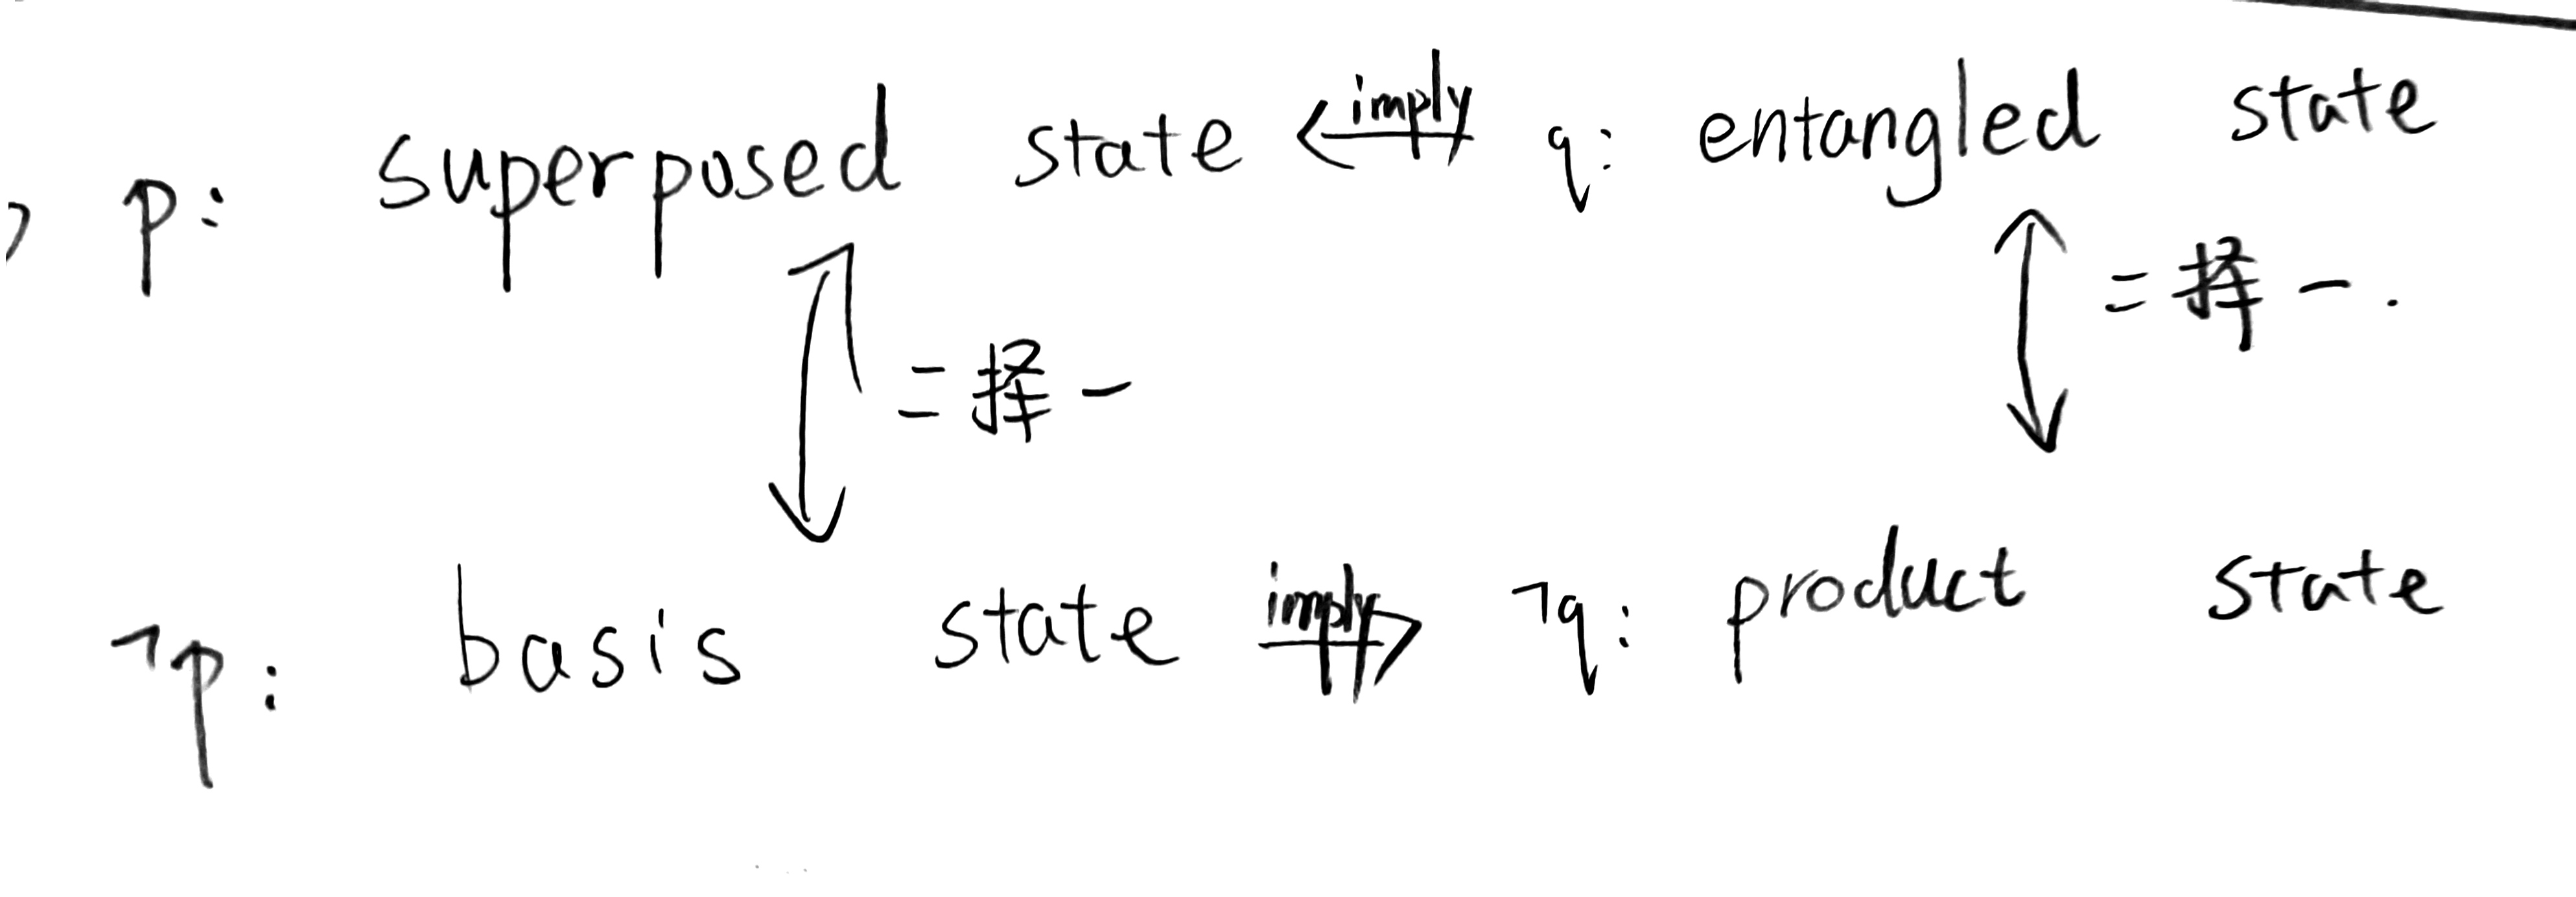
\includegraphics[width=0.75\linewidth]{Images/relation-superposed-entangled.jpg}
\end{figure}
        \item Notice that when an $n$-qubit system is entangled, it makes no sense to speak about qubit number $k \in[n]$ because isolated qubits are not defined. 
    \end{itemize}
\end{remark}

\subsection{3 Variational quantum algorithms for optimization}

Some of the quantum algorithms that tackle combinatorial optimization problems are Variational\footnote{The word "variational" does not have that mathematical meaning.} Quantum Algorithms (VQAs). They are hybrid algorithms because they require both quantum and classical computations. 

% VQAs are studied today because they represent an alternative approach that reduces the quality and quantity of the quantum resources needed. Specifically, they are designed to run on the \textbf{NISQ era} where quantum computers are noisy with few qubits: for instance, they harness \textit{low-depth quantum circuits}.

In this section, we consider optimization problems of the form
\begin{equation*}
\min _{x \in\{0,1\}^{n}} f(x), \tag{1}
\end{equation*}
where $f$ is any function defined on $\{0,1\}^{n}$. We note $\mathcal{F}$ the set of optimal solutions.

\subsubsection{General description}

Variational Quantum Algorithms (VQAs) are hybrid algorithms that, given an input $|0\rangle^{\otimes n}$, alternate between a quantum and a classical part. 
% Henceforth, we note $\left|0_{n}\right\rangle$ the state $|0\rangle^{\otimes n}$ to ease the reading. 

Let us first provide a high-level description of the key elements of VQAs that are detailed in this section. Let $d \in \mathbb{N}$, the three key elements of VQAs are:

\begin{itemize}
  \item a \textbf{parametrized quantum circuit}, $U: \mathbb{R}^{d} \rightarrow \mathcal{M}_{2^{n}}(\mathbb{C})$,
  \item a \textbf{guiding function}, $g: \mathbb{R}^{d} \rightarrow \mathbb{R}$,
  \item and a \textbf{classical optimizer}, which is an algorithm $\mathcal{A}$ that optimizes $g$ over space $\mathbb{R}^{d}$.
\end{itemize}

Before that, we provide a general overview of VQAs in Algorithm 1. 
\begin{figure}
    \centering
    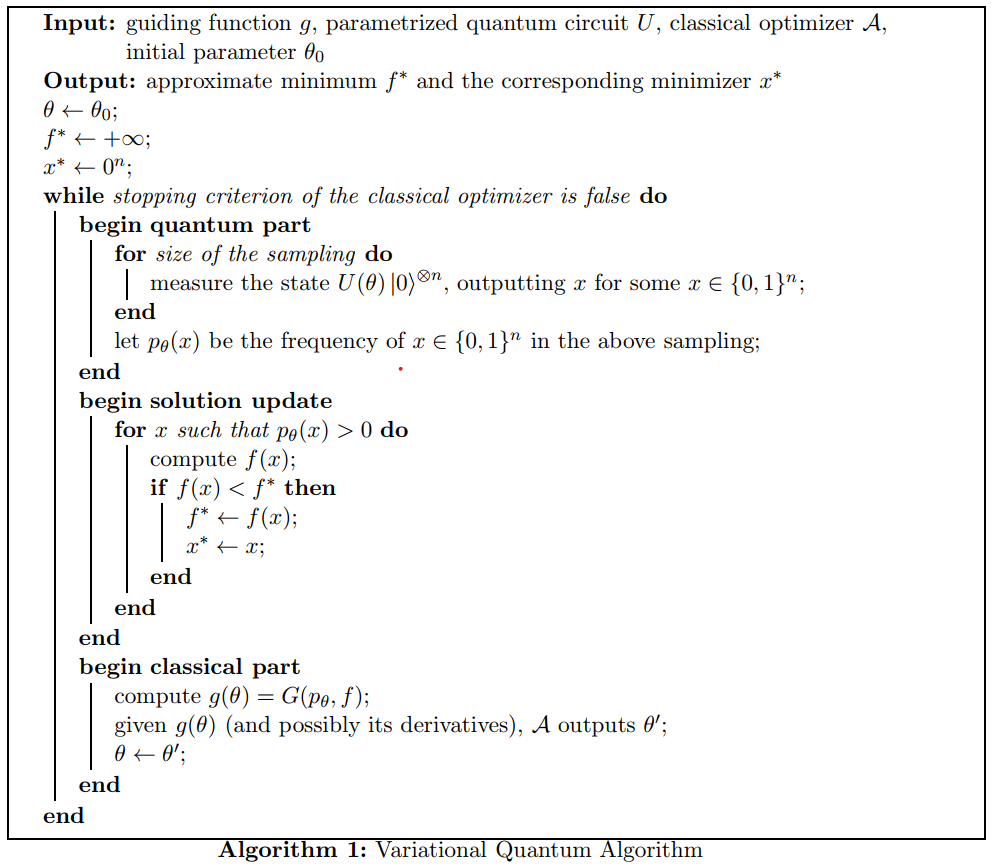
\includegraphics[width=1\linewidth]{Images/VQA-algorithm.png}
\end{figure}

The main idea of a VQA is as follows. The main loop of the algorithm executes the following steps until the classical optimizer stops according to a given stopping criterion. 

\begin{enumerate}
    \item (Quantum part) First, given $\theta \in \mathbb{R}^{d}$, the quantum part executes the parametrized quantum circuit $U(\theta)$ for several times to sample the quantum state. It results in a distribution probability over $\{0,1\}^{n}$ that we note $\left\{p_{\theta}(x): x \in\{0,1\}^{n}\right\}$. % 应该是简单的频率frequency统计
    \item (Classical part) Second, the classical part computes the cost of this state through the evaluation of the guiding function, according to the sampling results $p_{\theta}$, specifically, $g(\theta)=G\left(p_{\theta}, f\right)$ for a given function $G$ that is constructed from $f$ and $p_{\theta}$. More precisely, for a given $\theta$, the computation of $G$ requires only the values $f(x)$ for $x$ such that $p_{\theta}(x)>0$. % 我们不可能把所有f(x)算出了,否则直接比大小就完事了
    \item (Classical part) Eventually, this cost value is given to the classical optimizer $\mathcal{A}$, which outputs a new parameter in order to minimize $g$. % 可以用一些零阶优化技术
% Notice that, between the two parts the best-found solution is possibly updated by a classical computer.
\end{enumerate}

In the following subsections, we detail each part of VQAs and show \textbf{how specific choices of $g$ and $U$} \textbf{ensure that VQAs optimize $f$}.

\subsubsection{Quantum part}

The quantum part of VQAs applies a quantum circuit on the $n$-qubit system that constitutes the quantum computer. Importantly, \textit{variational}\footnote{The word "variational" does not have that mathematical meaning.}  in VQAs stands for the parametrization of the quantum circuit. 

Let $d \in \mathbb{N}$ be the number of parameters, thus $\theta \in \mathbb{R}^d.$

A \textit{parametrized quantum circuit} is a continuous function $U: \mathbb{R}^{d} \rightarrow$ $\mathcal{M}_{2^{n}}(\mathbb{C})$ mapping any $\theta \in \mathbb{R}^{d}$ to unitary matrix $U(\theta)$.

% As defined in Sect. 2.3, a quantum circuit is a sequence of universal quantum gates' compositions and/or tensor products. Thus, all coefficients of matrix $U(\theta)$ are continuous functions on $\mathbb{R}^{d}$.

Example 22 A simple example of a parametrized quantum circuit for $n=3$ and $d=3$ is depicted in Fig. 6.
\begin{figure}
    \centering
    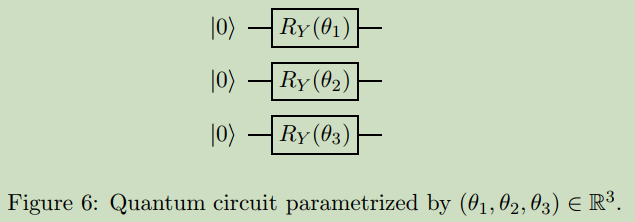
\includegraphics[width=0.75\linewidth]{Images/parametrized-quantum-circuit.png}
\end{figure}


\subsubsection{Classical part}

The classical part of VQAs consists of a classical optimization over the parameters $\theta \in \mathbb{R}^{d}$. 

\textbf{The classical optimizer essentially aims at finding the optimal parameters $\theta^{*}$ that lead to optimal solutions of the initial problem (1) with high probability}, specifically, such that
\begin{equation*}
\sum_{s \in \mathcal{F}}\left|\left\langle s\left|U\left(\theta^{*}\right)\right| 0_{n}\right\rangle\right|^{2} \geq 1-\epsilon \tag{10}
\end{equation*}
for small $\epsilon>0$. 

\begin{remark}
    \begin{itemize}
        \item We note $\mathcal{F}$ the set of optimal solutions in problem (1). We allow $\mathcal{F}$ to contain many different optimal solutions.
        \item  We note $\left|0_{n}\right\rangle$ the state $|0\rangle^{\otimes n}$ to ease the reading. Here, $0_{n}=000\dots0.$
        \item $U\left(\theta\right)| 0_{n}\rangle$ is the output state of the parametrized quantum circuit. 
        \item Note that we encode each possible optimization of (1), i.e, the n-bitstring, to basis state of quantum state space.
        \item We use notation $|s\rangle$ instead of $|i\rangle$ to efficiently recall that we deal with solutions of optimization problems (1). In fact, $\mathcal{F} \subset \{0,1\}^{n}$ and we use $s$ to denote the elements of $\mathcal{F}.$
        \item   In fact, we measure the output state by using the computational basis. In this paper, they are $\mathcal{C B}_{n}=\left\{|i\rangle, i \in\{0,1\}^{n}\right\}$.
        \item $\left|\left\langle s\left|U\left(\theta^*\right)\right| 0_n\right\rangle\right|^2$ is the probability with outcome $s$ after measurement. Then, $\sum_{s \in \mathcal{F}}\left|\left\langle s\left|U\left(\theta^{*}\right)\right| 0_{n}\right\rangle\right|^{2}$ is the probability with arbitrary optimal solutions after measurement.
    \end{itemize}
\end{remark}

The classical part is characterized by two aspects: 
\begin{enumerate}
    \item the function that guides the optimization
    \item the optimizer itself.
\end{enumerate}

\subsubsection{Guiding function}

Let $g: \mathbb{R}^{d} \rightarrow \mathbb{R}$ be the guiding function, formally defined in Definition 24 below, that the classical optimizer minimizes. 

\textbf{The function $g$ acts as a link between the quantum and classical parts. }

% For a given $\theta \in \mathbb{R}^{d}$, we evaluate $U(\theta)\left|0_{n}\right\rangle$ according to $f$ as we will exemplify below. Notice that $f$ and $g$ are distinct since $g$ is defined on $\mathbb{R}^{d}$ and outputs a quality measure of an $n$-qubit quantum state whereas $f$ is defined on $\{0,1\}^{n}$. 

Let us denote 
$$
\mathcal{F}_{\text {quant }}=\left\{\sum_{s \in \mathcal{F}} \psi_{s}|s\rangle: \sum_{s \in \mathcal{F}}\left|\psi_{s}\right|^{2}=1\right\}
$$
as the set of quantum states that are superpositions of optimal solutions of problem (1). %注意,F_{quant}所有对应原问题最优解的基态的线性组合(叠加态);所以如果我们测量F_{quant}里面的任意一个state,我们的结果都会是原优化问题的最优解。

\textbf{Naturally, we would like to define $g$ such that minimizing $g$ tends to minimize $f$.}

\begin{definition}[Guiding function]
    Definition 24 (Guiding function) Let $g: \mathbb{R}^{d} \rightarrow \mathbb{R}$ be a function and $\mathcal{G}$ be its set of minimizers. We call $g$ \textit{a guiding function for $f$ with respect to $U$} if $g$ is continuous and
\begin{equation*}
\left\{U(\theta)\left|0_{n}\right\rangle: \theta \in \mathcal{G}\right\} \subseteq \mathcal{F}_{\text {quant }} \tag{11}
\end{equation*}
\end{definition}

\begin{itemize}
    \item Indeed, Equation (11) implies that measuring the quantum state $U\left(\theta\right)|0\rangle^{\otimes n}$ for any $\theta\in \mathcal{G}$ outputs with probability 1 an optimal solution of the initial problem $s \in \mathcal{F}$.
    \item In other words, optima of a guiding function $g$ must lead to optima of $f$ or superpositions of optima of $f$.
    \item Thus, minimizing $f$ amounts to minimizing $g$, and finding $\mathcal{F}$ is done by finding $\mathcal{G}$. The latter is found with the classical optimizer.
\end{itemize}

% 下面两个remark亟需解决!

\begin{remark}
    Without any information on $\mathcal{F}$, we need to choose a quantum circuit $U$ such that any optimal solution $s \in \mathcal{F}$ is reachable, specifically, we construct $U$ such that
\begin{equation*}
\left\{U(\theta)\left|0_{n}\right\rangle: \theta \in \mathbb{R}^{d}\right\} \supseteq \mathcal{C} \mathcal{B}_{n} \supseteq \mathcal{F}. \tag{12}
\end{equation*}
Notice that this condition is weak and easily satisfied. For instance, the circuit depicted in Fig. 6 satisfies this condition. % 这段话暗示了,U的构造也需要精心设计的。
\end{remark}

\begin{remark}
If ever one is interested in finding all optimal solutions of problem (1), the circuit and the guiding function should satisfy instead the stronger condition than (11)
\begin{equation*}
\left\{U(\theta)\left|0_{n}\right\rangle: \theta \in \mathcal{G}\right\}=\mathcal{F}_{\text {quant}}. \tag{13}
\end{equation*}
In that case, $U$ satisfying (12) is not enough. Without any information on $\mathcal{F}$, we need to choose $U$ that can reach any $n$-qubit quantum states, specifically, % 这段话暗示了,U的构造也需要精心设计的。
$$
\left\{U(\theta)\left|0_{n}\right\rangle: \theta \in \mathbb{R}^{d}\right\}=\left\{\sum_{x \in\{0,1\}^{n}} \psi_{x}|x\rangle: \sum_{x \in\{0,1\}^{n}}\left|\psi_{x}\right|^{2}=1\right\}
$$
% 上式右侧是全部整个quantum state space!
\end{remark}

\begin{definition}[Mean function is a guiding function]
A popular choice for the guiding function in the literature is the \textit{mean function}
\begin{equation*}
g_{\text {mean }}(\theta)=\sum_{x \in\{0,1\}^{n}} p_{\theta}(x) f(x), \tag{14}
\end{equation*}
where
$$
p_{\theta}(x)=\left|\left\langle x|U(\theta)| 0_{n}\right\rangle\right|^{2}
$$
is the probability of finding $x$ when $U(\theta)\left|0_{n}\right\rangle$ is measured.  % 注意,出定义中的概率p是理论上的精确概率.
\end{definition}

We find that, $\theta$ decides $U(\theta)$ (once we set up the construct of circuit); then, $\theta$ decides output state $U(\theta)\left|0_{n}\right\rangle$ (the input state is always $\left|0_{n}\right\rangle$); then, $\theta$ decides the probability distribution $\{p_{\theta}(x)\}_{x}$. On the other hand, the values of $f(x)$ are unrelated to $\theta.$ Finally, for fixed optimization problem $\min _{x \in\{0,1\}^{n}} f(x)$ and well-constructed quantum circuit $U(\theta)$, the mean function $g_{\text {mean }}(\theta)$ only is concerned about parameter $\theta.$ 

\begin{proposition}
    Proposition 25 Function $g_{\text {mean }}$ is a guiding function.
\end{proposition}

\begin{proof}
Let us prove that $g_{\text {mean }}$ is continuous.
Let $x \in\{0,1\}^{n}$. The function $\theta \mapsto$ $p_{\theta}(x)=\left|\left\langle x|U(\theta)| 0_{n}\right\rangle\right|^{2}$ is continuous, because each coefficient of $U(\theta)$ is continuous. Thus, because multiplication and addition preserve continuity, $g_{\text {mean }}$ is continuous.

We prove by contradiction that (11) holds.
Let $\theta \in \mathcal{G}$ and let us consider the quantum state $|\psi(\theta)\rangle=U(\theta)\left|0_{n}\right\rangle$. Its decomposition in the canonical basis is $|\psi(\theta)\rangle=\sum_{x \in\{0,1\}^{n}} \psi_{x}|x\rangle$ with $\psi_{x}=\langle x|\psi(\theta)\rangle$. %牢记x是index

Assume that there exists some $\theta$ such that $|\psi(\theta)\rangle \notin \mathcal{F}_{\text {quant }}$. By definition of $\mathcal{F}_{\text {quant }}$, there exists $x_{0} \in\{0,1\}^{n}$ such that $x_{0} \notin \mathcal{F}$ and $\left|\psi_{x_{0}}\right| \neq 0$ (nonzero coefficient). Thus,
$$
\begin{aligned}
g_{\text {mean }}(\theta) & =\sum_{x \in\{0,1\}^{n}}\left|\psi_{x}\right|^{2} f(x) \\
& =\sum_{x \in \mathcal{F}}\left|\psi_{x}\right|^{2} f(x)+\sum_{x \notin \mathcal{F}}\left|\psi_{x}\right|^{2} f(x) \\
& =\left(\sum_{x \in \mathcal{F}}\left|\psi_{x}\right|^{2}\right) f^{*}+\sum_{x \notin \mathcal{F}}\left|\psi_{x}\right|^{2} f(x)
\end{aligned}
$$
where $f^{*}$ is the optimal value of $f$, reached on $\mathcal{F}$. By definition, $f(x)>f^{*}, \forall x \notin \mathcal{F}$, and because we assume that $\left|\psi_{x_{0}}\right| \neq 0$, thus the second term of the sum is bounded below as follows: $\sum_{x \notin \mathcal{F}}\left|\psi_{x}\right|^{2} f(x)>\left(\sum_{x \notin \mathcal{F}}\left|\psi_{x}\right|^{2}\right) f^{*}$, where $\sum_{x \notin \mathcal{F}}\left|\psi_{x}\right|^{2} \geq$ $\left|\psi_{x_{0}}\right|^{2}>0$. Thus,
$$
g_{\text {mean }}(\theta)>\left(\sum_{x \in \mathcal{F}}\left|\psi_{x}\right|^{2}\right) f^{*}+\left(\sum_{x \notin \mathcal{F}}\left|\psi_{x}\right|^{2}\right) f^{*}=f^{*}
$$
This contradicts the previous statement that $\theta \in \mathcal{G}$, as one readily verifies that the infimum of $g_{\text {mean }}$ is $g_{\text {mean }}^{*}=f^{*}$.
% 这来自于一个简单的命题。考虑一些实数的凸组合(系数非负且和为一),那么它们组合的结果的上限是这些实数中的最大值,其下限是这些实数中的最小值。
\end{proof}

\begin{example}
    Example 26 We illustrate the mean function on the 3-qubit quantum circuit $U(\theta)$ depicted in Fig. 6. The generalization of its computation for $n$ qubits is trivial since it needs to replace 3 by $n$. 
    
The single application of rotation gate $R_{Y}$ (6) of angle $\theta_{i}$ on a qubit initially on state $|0\rangle$ is
$$
\begin{aligned}
R_{Y}\left(\theta_{i}\right)|0\rangle & =\cos \frac{\theta_{i}}{2}|0\rangle+\sin \frac{\theta_{i}}{2}|1\rangle \\
& =\sum_{j \in\{0,1\}} \cos \frac{\theta_{i}-j \pi}{2}|j\rangle
\end{aligned}
$$
since $\sin (\phi)=\cos \left(\phi-\frac{\pi}{2}\right)$ for any $\phi \in \mathbb{R}$. Eventually, the quantum state resulting from $U(\theta)$ is
$$
\begin{aligned}
U(\theta)\left|0_{3}\right\rangle & =\bigotimes_{i=1}^{3} R_{Y, i}\left(\theta_{i}\right)|0\rangle \\
& =\sum_{j_{1}, j_{2}, j_{3} \in\{0,1\}}\left(\prod_{i=1}^{3} \cos \frac{\theta_{i}-j_{i} \pi}{2}\right)\left|j_{1} j_{2} j_{3}\right\rangle
\end{aligned}.
$$
Thus, the probability to measure $x=\left(x_{1}, x_{2}, x_{3}\right) \in\{0,1\}^{3}$ is
\begin{equation*}
p_{\theta}(x)=\left(\prod_{i=1}^{3} \cos \frac{\theta_{i}-x_{i} \pi}{2}\right)^{2} \tag{15}
\end{equation*}
and the expression of $g_{\text {mean }}$ of equation (14) directly results from it.
\end{example}



\subsubsection{Classical optimizer} % 需要复习一下概率论,请先阅读

The role of the classical optimizer is to minimize the guiding function. The function $g$ is continuous and is usually differentiable but \textit{not convex}. Any unconstrained optimization algorithm can be used to minimize $g$.

\textbf{To speak in terms of stochastic optimization}, the classical optimizer aims at solving the stochastic programming model under \textit{endogenous uncertainty} 
\begin{equation*}
\min _{\theta}\left\{g(\theta)=\mathbb{E}_{\xi_{\theta} \sim p_{\theta}}\left[G\left(\theta, \xi_{\theta}\right)\right]\right\} \tag{19}
\end{equation*}
where the definition of $G$ depends on the choice of a specific guiding function $g$, and $\xi_{\theta}$ is an endogenous random variable that depends on $\theta$. Specifically, $\xi_{\theta}$ is a discrete random variable, with the set of possible outcomes $\{0,1\}^{n}$ and the following distribution probability:
$$
\mathbb{P}\left(\xi_{\theta}=x\right)=p_{\theta}(x), \quad \forall x \in\{0,1\}^{n}.
$$
\begin{example}
    For instance, for the case of $g=g_{\text {mean }}$, we have
$$
G\left(\theta, \xi_{\theta}\right)=f\left(\xi_{\theta}\right).
$$
Then, 
$$
g_{\text {mean }}(\theta)
=\mathbb{E}_{\xi_{\theta} \sim p_{\theta}}\left[f\left(\xi_{\theta}\right)\right]
=\sum_{x \in\{0,1\}^{n}} p_{\theta}(x) f(x).
$$
\end{example}

\todo{How to consider the another guiding function --- Gibbs function?}

The problem (19) falls into the class of \textbf{stochastic dependent-decision probabilities problems}. % 目前的理解是,在式(19)中,theta决定了随机变量xi_theta,通过期望的计算消除了该随机变量的随机性。但外从外部看,其整体是依赖于变量theta。
In practice, the classical optimizer approximates the value of objective function $g(\theta)$ by a \textit{Monte Carlo estimation} as follows:
$$
\hat{g}_{N}(\theta)=\frac{1}{N} \sum_{j=1}^{N} G\left(\theta, \xi_{\theta}^{j}\right)
$$
where $\left\{\xi_{\theta}^{j}\right\}_{j \in[N]}$ is a sample of size $N$ from the distribution of $\xi_{\theta}$. Notice that for a given $\theta$, the quantity $\hat{g}_{N}(\theta)$ itself is a random variable since its value depends on the sample that has been generated, which is random. In contrast, the value of $g(\theta)$ is deterministic. Notice that according to the Law of Large Numbers, $\hat{g}_{N}(\theta)$ converges with probability one to $g(\theta)$ as $N \rightarrow \infty$.

\begin{example}
For instance, for the case of $g=g_{\text {mean }}$, we have
$$
G\left(\theta, \xi_{\theta}\right)=f\left(\xi_{\theta}\right)
$$
Hence, for each $\xi_{\theta}^{j} \in\{0,1\}^{n}$ sampled, either we compute classically $f(\xi_{\theta}^{j})$ and store it if not already computed, or we get its value. Thus, we can compute $\hat{g}_{N}(\theta)$. 
\end{example}

\subsection{4 Quantum approximate optimization algorithm}

We assume throughout this section that the function $f$ to be minimized is \textit{polynomial}. Actually, it is multilinear polynomial.

First, we reformulate problem (1) to a more suitable form for quantum optimization. This reformulation is motivated by the \textit{quantum adiabatic evolution} that, for a given Hermitian matrix, approximates the eigenvector with the lowest eigenvalue under certain conditions. 

For that, we interpret the objective function of problem (1) as an Hermitian matrix $H_{f}$ such that each eigenvector $\left|u_{x}\right\rangle$ is matching a classical solution $x \in\{0,1\}^{n}$ with an eigenvalue equal to $f(x)$, specifically,
$$
H_{f}\left|u_{x}\right\rangle=f(x)\left|u_{x}\right\rangle .
$$
\textbf{Thus, the solutions of problem (1) are the solutions corresponding to the lowest eigenvalues of $H_{f}$.} \textbf{The Quantum Approximate Optimization Algorithm (QAOA) presented in this section aims at finding the lowest eigenvalue of $H_{f}$.} % 本节概括

\subsubsection{Problem reformulation}

The construction of $H_{f}$ is as follows. 

First, we transform the $\{0,1\}$ problem (1) into a $\{-1,1\}$-problem. For that, we apply the following linear transformation: for $x=$ $\left(x_{1}, \ldots, x_{n}\right) \in\{0,1\}^{n}$, we define $z=\left(z_{1}, \ldots, z_{n}\right) \in\{-1,1\}^{n}$ where
\begin{equation*}
z_{i}=1-2 x_{i}, \forall i \in[n]. \tag{20}
\end{equation*}
(Note that $x_{i}=0$ iff $z_i=1$ and $x_{i}=1$ iff $z_i=-1.$) This leads to the problem
$$
\min _{z \in\{-1,1\}^{n}} f_{ \pm}(z)
$$
where, for $z \in\{-1,1\}^{n}$,
$$
f_{ \pm}(z)=\sum_{\alpha=\left(\alpha_{1}, \ldots \alpha_{n}\right) \in\{0,1\}^{n}} h_{\alpha} \prod_{i=1}^{n} z_{i}^{\alpha_{i}}
$$
where $h_{\alpha} \in \mathbb{R}, \forall \alpha \in\{0,1\}^{n}$. Recall that we assumed $f$ to be \textit{multilinear polynomial}. %通过(20)这样子简单的换元操作,multilinear polynomial在数学形式上是不变的。请参考Example 33。

Second, we define the $2^n$ by $2^n$ matrix $H_{f}$ (called "Hamiltonian") as
$$
H_{f}:=\sum_{\alpha=\left(\alpha_{1}, \ldots \alpha_{n}\right) \in\{0,1\}^{n}} h_{\alpha} \bigotimes_{i=1}^{n} Z_{i}^{\alpha_{i}}
$$
where $Z=\left(\begin{array}{cc}1 & 0 \\ 0 & -1\end{array}\right), Z^{0}=I$ and $Z^{1}=Z$. \textbf{We note $Z_{i}$ the application of $Z$ to qubit $i$. } % number z --> gate Z; product --> tensor product

Note that the tensor product of Hermitian matrices is also Hermitian, and the $\mathbb{R}$-linear combination of Hermitian matrices is again Hermitian. Hence, $H_{f}$ above is Hermitian.

Notice that $Z$ is equal to the universal gate $R_{Z}(\pi)$ modulo a global phase (see (7)). This construction of $H_{f}$ leads to the following property.

\begin{proposition}
    Proposition 32 The eigenvectors of $H_{f}$ are the canonical basis $|x\rangle \in \mathcal{C B}_{n}$ with eigenvalues that are the cost of the solutions $f(x)$, specifically,
\begin{equation*}
\forall|x\rangle \in \mathcal{C B}_{n}, \quad H_{f}|x\rangle=f(x)|x\rangle. \tag{21}
\end{equation*}
\end{proposition}
\begin{proof}
    First, the eigenvectors of $H_{f}$ are the canonical basis states. Indeed, each term of the sum that constitutes $H_{f}$ is a tensor product of $n$ matrices $I$ or $Z$, both diagonal\footnote{The tensor product of two diagonal matrices is also diagonal}. Thus, $H_{f}$ is a $2^{n}$ diagonal matrix. 
    
    Second, let us find the eigenvalues associated with the eigenvectors. Let $|x\rangle=\left|x_{1} \ldots x_{n}\right\rangle$ be in $\mathcal{C B}_{n}$. Let $z=\left(z_{1}, \ldots, z_{n}\right)$ be the result of transformation (20). Thus, we can easily show that 
$$
Z^{0}\left|x_{i}\right\rangle=I\left|x_{i}\right\rangle=z_{i}^{0}\left|x_{i}\right\rangle,Z^{1}\left|x_{i}\right\rangle=Z\left|x_{i}\right\rangle=z_{i}^{1}\left|x_{i}\right\rangle, \forall i \in[n],
$$
and
$$
\begin{aligned}
H_{f}|x\rangle 
& =\left(\sum_{\alpha=\left(\alpha_{1}, \ldots \alpha_{n}\right) \in\{0,1\}^{n}} h_{\alpha} \bigotimes_{i=1}^{n} Z_{i}^{\alpha_{i}}\right) \left|x_{1} \ldots x_{n}\right\rangle\\
& =\sum_{\alpha=\left(\alpha_{1}, \ldots \alpha_{n}\right) \in\{0,1\}^{n}} h_{\alpha} \left(\bigotimes_{i=1}^{n} Z_{i}^{\alpha_{i}}\right) \left|x_{1} \ldots x_{n}\right\rangle\\
& =\sum_{\alpha=\left(\alpha_{1}, \ldots, \alpha_{n}\right) \in\{0,1\}^{n}} h_{\alpha} \left( \bigotimes_{i=1}^{n} Z_{i}^{\alpha_{i}}\left|x_{i}\right\rangle\right) \\
& =\sum_{\alpha=\left(\alpha_{1}, \ldots, \alpha_{n}\right) \in\{0,1\}^{n}} h_{\alpha} \left(\bigotimes_{i=1}^{n} z_{i}^{\alpha_{i}}\left|x_{i}\right\rangle\right) \\
& =\sum_{\alpha=\left(\alpha_{1}, \ldots, \alpha_{n}\right) \in\{0,1\}^{n}} h_{\alpha} \left(\prod_{i=1}^{n} z_{i}^{\alpha_{i}}\left|x_{i}\right\rangle\right) \\
& =\sum_{\alpha=\left(\alpha_{1}, \ldots \alpha_{n}\right) \in\{0,1\}^{n}} h_{\alpha} \left(\prod_{i=1}^{n} z_{i}^{\alpha_{i}}\right) \left|x_{1} \ldots x_{n}\right\rangle\\
& =\left(\sum_{\alpha=\left(\alpha_{1}, \ldots, \alpha_{n}\right) \in\{0,1\}^{n}} h_{\alpha} \prod_{i=1}^{n} z_{i}^{\alpha_{i}}\right)|x\rangle \\
& =f_{ \pm}(z)|x\rangle \\
& =f(x)|x\rangle .
\end{aligned}
$$
\end{proof}
\begin{example}
    Example 33 We illustrate this transformation on a small example with $n=2$. Let us consider the problem
$$
\min _{x \in\{0,1\}^{2}} f(x)=x_{1}+2 x_{2}-3 x_{1} x_{2}
$$
Using (20), the equivalent $\{-1,1\}$-problem is
$$
\min _{z \in\{-1,1\}^{2}} f_{ \pm}(z)=\frac{1}{4} z_{1}-\frac{1}{4} z_{2}-\frac{3}{4} z_{1} z_{2}+\frac{3}{4}
$$
Thus, the Hermitian matrix associated with the problem is
$$
H_{f}=\frac{1}{4} Z \otimes I-\frac{1}{4} I \otimes Z-\frac{3}{4} Z \otimes Z+\frac{3}{4} I \otimes I
$$
To illustrate (21), we compute the eigenvalue of the canonical basis state $|10\rangle$.
$$
\begin{aligned}
H_{f}|10\rangle & =\frac{1}{4}(Z \otimes I)|10\rangle-\frac{1}{4}(I \otimes Z)|10\rangle-\frac{3}{4}(Z \otimes Z)|10\rangle+\frac{3}{4}(I \otimes I)|10\rangle \\
& =-\frac{1}{4}|10\rangle-\frac{1}{4}|10\rangle+\frac{3}{4}|10\rangle+\frac{3}{4}|10\rangle \\
& =|10\rangle \\
& =f(1,0)|10\rangle
\end{aligned}
$$
because $f(1,0)=1$.
\end{example}

Notice that most of the problems solved with QAOA in the literature are QUBO (Quadratic Unconstrained Binary Optimization) problems. Thus, $H_{f}$ has the specific form
$$
H_{f}=\sum_{i} h_{i i} Z_{i}+\sum_{i<j} h_{i j} Z_{i} \otimes Z_{j}
$$
where $h_{i j} \in \mathbb{R}, \forall i \leq j$. Note that $Z_{i}$ the application of $Z$ to qubit $i$. As mentioned before, we use the notation $Z_{i}$ for the application of $Z$ on qubit $i$ (and the application of identity matrix on the remaining qubits). Like in Example 33, $Z_1=Z \otimes I$ and $Z_2=I \otimes Z$.


It is justified by the fact that solving QUBO problems to optimality is already NP-hard, and the quantum gates of the circuit are easier to implement on hardware in that case.

\href{https://ww2.mathworks.cn/help/matlab/math/what-is-a-qubo.html}{What Is a QUBO Problem? - MATLAB \& Simulink - MathWorks} 

\subsubsection{Quantum part}

\textbf{QAOA is a Variational Quantum Algorithm where the quantum part derives from the Hamiltonian $H_{f}$. }

This quantum part consists of a quantum circuit with $2 p$ parameters $(\boldsymbol{\gamma}, \boldsymbol{\beta})=\left(\gamma_{1}, \ldots, \gamma_{p}, \beta_{1}, \ldots, \beta_{p}\right) \in \mathbb{R}^{2 p}$, where $p$ is called \textit{depth}. 

\begin{definition}
    Definition 43 (Unitary operator associated with Hermitian matrix) Given a Hermitian matrix $A$, we define its associated quantum gate $\operatorname{Exp}(A, t)$ parametrized by the parameter $t \in \mathbb{R}$ as:
$$
\begin{aligned}
\operatorname{Exp}(A, t) & =e^{-i A t} \\
& =\sum_{k=0}^{\infty} \frac{1}{k!}(-i)^{k} t^{k} A^{k}
\end{aligned}
$$
Because $A$ is Hermitian, $\operatorname{Exp}(A, t)$ is a unitary matrix.
\end{definition}

The quantum circuit $U(\boldsymbol{\gamma}, \boldsymbol{\beta})$ is the sequence of $p$ layers of two blocks, initially applied to the uniform superposition $|+\rangle^{\otimes n}$. % the sequence of $p$ layers of two blocks , 意思就是两个一组,一共有p组在一起。
\begin{itemize}
    \item The first block is of the form $\operatorname{Exp}\left(H_{f}, \gamma\right)$, for $\gamma \in \mathbb{R}$, which is the unitary operator associated with the Hamiltonian $H_{f}$.
    \item The second block is of the form $\operatorname{Exp}\left(H_{B}, \beta\right)$, for $\beta \in \mathbb{R}$, which is the unitary operator associated with the Hamiltonian
    $$
  H_{B}=\sum_{i=1}^{n} R_{X, i}(\pi).
  $$
\end{itemize}
Thus, the quantum circuit is
\begin{equation*}
U(\boldsymbol{\gamma}, \boldsymbol{\beta})=\operatorname{Exp}\left(H_{B}, \beta_{p}\right) \operatorname{Exp}\left(H_{f}, \gamma_{p}\right) \ldots \operatorname{Exp}\left(H_{B}, \beta_{1}\right) \operatorname{Exp}\left(H_{f}, \gamma_{1}\right) H^{\otimes n} \tag{22}
\end{equation*}
where the first gates applied in this circuit are $H^{\otimes n}$m, to then apply the $p$ layers to state $|+\rangle^{\otimes n}$. 

The three propositions that follow express the quantum circuit of QAOA with the set of universal gates (see Theorem 13). We give first the general decomposition of the QAOA quantum circuit defined in (22), see Appendix B.2.1 for a proof.

\begin{proposition}
    Proposition 34 The first block $\operatorname{Exp}\left(H_{f}, \gamma\right)$ parametrized by $\gamma \in \mathbb{R}$ is
$$
\operatorname{Exp}\left(H_{f}, \gamma\right)=\prod_{\alpha \in\{0,1\}^{n}} \operatorname{Exp}\left(\bigotimes_{i=1}^{n} Z_{i}^{\alpha_{i}}, h_{\alpha} \gamma\right)
$$
The second block $\operatorname{Exp}\left(H_{B}, \beta\right)$ parametrized by $\beta \in \mathbb{R}$ is
$$
\operatorname{Exp}\left(H_{B}, \beta\right)=\bigotimes_{i=1}^{n} R_{X, i}(2 \beta)
$$
\end{proposition}

\begin{remark}
    The Kronecker sum satisfies the nice property
$$
\exp (A) \otimes \exp (B)=\exp (A \oplus B)
$$
(Horn and Johnson 1994, p. 208).
$$
e^{\mathrm{A}} e^{\mathrm{B}}=e^{\mathrm{A}+\mathrm{B}}
$$
holds only when $A$ and $B$ commute, i.e.,$[A, B]=A B-B A=0.$
\end{remark}

\begin{proof}
Let $\gamma \in \mathbb{R}$ and let us consider the first block $\operatorname{Exp}\left(H_{f}, \gamma\right)$. By Definition 43, and because each pair of matrices of the family $\left\{\bigotimes_{i=1}^{n} Z_{i}^{\alpha_{i}}: \alpha=\left(\alpha_{1}, \ldots, \alpha_{n}\right) \in\{0,1\}^{n}\right\}$ commutes two by two, %two by two 两个一组地
\begin{align*}
\operatorname{Exp}\left(H_{f}, \gamma\right) & =e^{-i\left(\sum_{\alpha=\left(\alpha_{1}, \ldots, \alpha_{n}\right) \in(0,1)^{n}} h_{\alpha} \bigotimes_{i=1}^{n} Z_{i}^{\alpha_{i}}\right) \gamma}  \tag{23}\\
& =\prod_{\alpha=\left(\alpha_{1}, \ldots, \alpha_{n}\right) \in\{0,1\}^{n}} e^{-i h_{\alpha} \bigotimes_{i=1}^{n} Z_{i}^{\alpha_{i}} \gamma}  \tag{24}\\
& =\prod_{\alpha=\left(\alpha_{1}, \ldots, \alpha_{n}\right) \in\{0,1\}^{n}} \operatorname{Exp}\left(\bigotimes_{i=1}^{n} Z_{i}^{\alpha_{i}}, h_{\alpha} \gamma\right). \tag{25}
\end{align*}

Let $\beta \in \mathbb{R}$ and let us consider the second block $\operatorname{Exp}\left(H_{B}, \beta\right)$. For more readability, we write $X_{i}=R_{X, i}(\pi)$, the application of matrix $X=\left(\begin{array}{ll}0 & 1 \\ 1 & 0\end{array}\right)$ on qubit $i$. With the same development as above, and because each pair of matrices of the family $\left\{X_{i}: i \in[n]\right\}$ commutes two by two,
$$
\operatorname{Exp}\left(H_{B}, \beta\right)=\prod_{i=1}^{n} \operatorname{Exp}\left(X_{i}, \beta\right)
$$
Let $i \in[n]$. Thus,
\begin{align*}
\operatorname{Exp}\left(X_{i}, \beta\right) & =\sum_{k=0}^{\infty} \frac{1}{k!}(-i)^{k} \beta^{k} X_{i}^{k}  \tag{26}\\
& =\sum_{k=0}^{\infty} \frac{1}{(2 k)!}(-i)^{2 k} \beta^{2 k} X_{i}^{2 k}+\sum_{k=0}^{\infty} \frac{1}{(2 k+1)!}(-i)^{(2 k+1)} \beta^{(2 k+1)} X_{i}^{(2 k+1)} \tag{27} \\
& =\sum_{k=0}^{\infty} \frac{1}{(2 k)!}(-i)^{2 k} \beta^{2 k} I+\sum_{k=0}^{\infty} \frac{1}{(2 k+1)!}(-i)^{(2 k+1)} \beta^{(2 k+1)} X_{i}  \tag{28}\\
& =\sum_{k=0}^{\infty} \frac{1}{(2 k)!}(-1)^{k} \beta^{2 k} I-i \sum_{k=0}^{\infty} \frac{1}{(2 k+1)!}(-1)^{k} \beta^{(2 k+1)} X_{i}  \tag{29}\\
& =\cos (\beta) I-i \sin (\beta) X_{i}  \tag{30}\\
& =R_{X, i}(2 \beta) \tag{31}
\end{align*}
where line (28) exploits the fact that $X^{2}=I$, implying $X^{2 k}=I$ and $X^{2 k+1}=X$. Moreover, line (29) applies the definition of the complex number $i$, and one can recognize the power series of cosines and sinus functions.
\end{proof}

The particular case of QUBO is mainly considered in the literature. 

Thus, we propose next a decomposition of the QAOA quantum circuit for this specific case, see Appendix B.2.2 for a proof.

\begin{proposition}
    Proposition 35 For the case of QUBO, the expression of $\operatorname{Exp}\left(H_{f}, \gamma\right)$ simplifies in
$$
\operatorname{Exp}\left(H_{f}, \gamma\right)=\left(\bigotimes_{i=1}^{n} R_{Z, i}\left(2 h_{i i} \gamma\right)\right) \prod_{i<j} C X_{i, j} R_{Z, j}\left(2 h_{i, j} \gamma\right) C X_{i, j}
$$
and is rather easily implemented with universal quantum gates.
\end{proposition}

\begin{proof}
    Proof Let $\gamma \in \mathbb{R}$. The application of (23)-(25) to the case of QUBO gives
$$
\begin{aligned}
\operatorname{Exp}\left(H_{f}, \gamma\right) & =e^{-i\left(\sum_{i=1}^{n} h_{i i} Z_{i}+\sum_{i<j} h_{i j} Z_{i} \otimes Z_{j}\right) \gamma} \\
& =\prod_{i=1}^{n} e^{-i Z_{i} h_{i i} \gamma} \prod_{i<j} e^{-i Z_{i} \otimes Z_{j} h_{i j} \gamma} \\
& =\prod_{i=1}^{n} \operatorname{Exp}\left(Z_{i}, h_{i i} \gamma\right) \prod_{i<j} \operatorname{Exp}\left(Z_{i} \otimes Z_{j}, h_{i j} \gamma\right)
\end{aligned}
$$
Then, let us prove that, for $i \in[n]$ and $t \in \mathbb{R}, \operatorname{Exp}\left(Z_{i}, t\right)=R_{Z, i}(2 t)$. The same development as above (28)-(30), replacing $X$ by $Z$ that have the same property $Z^{2}=I$, gives
\begin{align*}
\operatorname{Exp}\left(Z_{i}, t\right) & =\cos (t) I-i \sin (t) Z_{i}  \tag{32}\\
& =R_{Z, i}(2 t) \tag{33}
\end{align*}
Eventually, line (32) is the application of the gate $\left(\begin{array}{cc}e^{-i t} & 0 \\ 0 & e^{i t}\end{array}\right)=R_{Z}(2 t)$ on qubit $i$, and the identity on the others.

It remains to prove that, for $i<j \in[n]$ and $t \in \mathbb{R}, \operatorname{Exp}\left(Z_{i} \otimes Z_{j}, t\right)=$ $C X_{i, j} R_{Z, j}(2 t) C X_{i, j}$. Following the same developments as above, we have
\begin{equation*}
\operatorname{Exp}\left(Z_{i} \otimes Z_{j}, t\right)=\cos (t) I-i \sin (t) Z_{i} \otimes Z_{j} \tag{34}
\end{equation*}
We consider the two-qubit system that corresponds to the qubit $i$ as the first qubit and the qubit $j$ as the second qubit (the others are unchanged by the transformation). Thus, it remains to prove the equality of the two circuits depicted on Fig. 9.
\begin{figure}
    \centering
    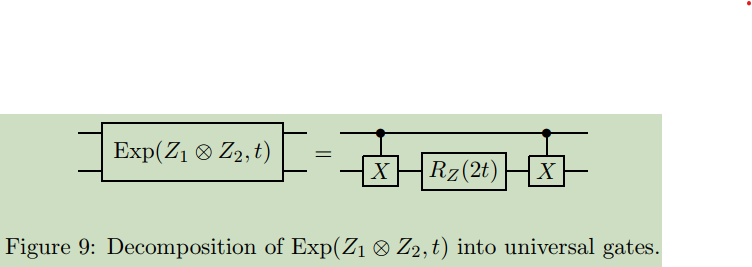
\includegraphics[width=0.75\linewidth]{Images/grange23-f9.png}
\end{figure}
On the one hand, (34) is the application of the gate $=\left(\begin{array}{cc}R_{Z}(2 t) & 0 \\ 0 & R_{Z}(-2 t)\end{array}\right)$ to this system. Indeed,

$$
\begin{aligned}
\cos (t) I-i \sin (t) Z_{1} \otimes Z_{2} & =\cos (t)\left(\begin{array}{llll}
1 & 0 & 0 & 0 \\
0 & 1 & 0 & 0 \\
0 & 0 & 1 & 0 \\
0 & 0 & 0 & 1
\end{array}\right)-i \sin (t)\left(\begin{array}{cccc}
1 & 0 & 0 & 0 \\
0 & -1 & 0 & 0 \\
0 & 0 & -1 & 0 \\
0 & 0 & 0 & 1
\end{array}\right) \\
& =\left(\begin{array}{cccc}
e^{-i t} & 0 & 0 & 0 \\
0 & e^{i t} & 0 & 0 \\
0 & 0 & e^{i t} & 0 \\
0 & 0 & 0 & e^{-i t}
\end{array}\right) \\
& =\left(\begin{array}{ccc}
R_{Z}(2 t) & 0 & \\
0 & R_{Z}(-2 t)
\end{array}\right) .
\end{aligned}
$$

On the other hand, the composition of gates $C X_{1,2} R_{Z, 2}(2 t) C X_{1,2}$ on this system amounts to
$$
\begin{aligned}
C X_{1,2} R_{Z, 2}(2 t) C X_{1,2} & =\left(\begin{array}{cc}
I & 0 \\
0 & X
\end{array}\right)\left(\begin{array}{cc}
R_{Z}(2 t) & 0 \\
0 & R_{Z}(2 t)
\end{array}\right)\left(\begin{array}{ll}
I & 0 \\
0 & X
\end{array}\right) \\
& =\left(\begin{array}{cc}
R_{Z}(2 t) & 0 \\
0 & X R_{Z}(2 t) X
\end{array}\right) \\
& =\left(\begin{array}{cc}
R_{Z}(2 t) & 0 \\
0 & R_{Z}(-2 t)
\end{array}\right) .
\end{aligned}
$$
Thus, the proof results from replacing $t$ by appropriate values $h_{i i} \gamma$ for $i \in[n]$ and $h_{i j} \gamma$ for $i<j$.
\end{proof}

The decomposition in universal quantum gates of the term $\operatorname{Exp}\left(Z_{i} \otimes Z_{j}, t\right)$ for the specific case of QUBO (see Proposition 35) is mainly used in the literature. 





%----------------------------------------------------------------------------------------
%	PART III
%----------------------------------------------------------------------------------------

% \part{Other Notes}

% %Simon Algorithm-------------------------------------------------------------------------
% \section{Simon Algorithm}
% \subsection{Boolean Function}
% \begin{definition}
A \textbf{boolean function} $F$ is defined as

$$
F:\{0,1\}^m \rightarrow\{0,1\}.
$$

A \textbf{vector-valued boolean function} $f$ is defined as

$$
f:\{0,1\}^m \rightarrow\{0,1\}^n.
$$
\end{definition}

A boolean function is a specific type of vector-valued boolean function when $n=1$. 

\begin{remark}
For any given $m$ and $n$, there exist $2^{(n \times 2^m)}$ distinct vector-valued boolean functions from $\{0,1\}^m$ to $\{0,1\}^n$.
\end{remark}

\begin{proof}
For any input value $\vec{x} \in \{0,1\}^m$, there are $2^n$ different possible output values $f(\vec{x}) \in \{0,1\}^n$. So the total number of distinct vector-valued boolean functions is 

$$
\underbrace{2^n \times 2^n \times \cdots \times 2^n}_{2^m}=2^{\left(n \times 2^m\right)}.
$$
\end{proof}

% \subsection{Simon's Problem}
% \begin{definition}\label{Simon's Problem}
Simon's \cite{simon1997power} problem is defined as follows: There exists a special vector-valued boolean function $f:\{0,1\}^n \rightarrow\{0,1\}^n$. Here $f$ satisfies the condition

$$
f(\vec{x})=f(\vec{y}) \iff \vec{y}=\vec{x}\oplus \vec{s},
$$ 
where $\vec{s}\in\{0,1\}^n$ is \textbf{unique}. Our objective is to determine the unique $\vec{s}$ by querying the function as few times as possible.
\end{definition}

\begin{remark}
"Querying the function" once means we give an input value $\vec{x} \in \{0,1\}^n$ to the computer and obtain its corresponding output value $f(\vec{x})$.
\end{remark}
	
\begin{mdframed}
	Given $\vec{a}=a_1a_2...a_n$ and $\vec{b}=b_1b_2...b_n$, where $a_i\in\{0,1\}$, $b_i\in\{0,1\}$, $i\in[n]$, $\vec{a}\oplus \vec{b}$ is defined as   
	\[
	\vec{a}\oplus \vec{b}=c_1c_2...c_n,
	\]
	where
	$$
	c_i=\left\{\begin{array}{ll}
		0 & \text { if } a_i = b_i, \\
		1 & \text { otherwise },
	\end{array} \forall i=1, \ldots, n.\right.
	$$
\end{mdframed}

%	According to the special vector-valued boolean function given by Simon, we can get
%	$$
%	\begin{aligned}
%		\vec{y} & =\vec{x} \oplus \vec{s}, \\
%		\vec{y} \oplus \vec{s} & =\vec{x} \oplus \vec{s} \oplus \vec{s}, \\
%		\vec{y} \oplus \vec{s} & =\vec{x} \oplus \overrightarrow{0}(\because \vec{s} \oplus \vec{s}=\overrightarrow{0}), \\
%		\vec{y} \oplus \vec{s} & =\vec{x}.
%	\end{aligned}
%	$$
	
\begin{property}
If $\vec{s}=\vec{0}$, the $f$ in \textbf{Definition} \ref{Simon's Problem} is \textbf{one-to-one}. In this case, there exist $2^n !$ distinct vector-valued boolean functions that satisfy the condition in \textbf{Definition} \ref{Simon's Problem}.
\end{property}

\begin{proof}
If $\vec{s} = \vec{0}$, we can get

$$
f(\vec{x})=f(\vec{y}) \iff \vec{y}=\vec{x}\oplus \vec{0} = \vec{x}.
$$

This implies that for any two distinct input values $\vec{\alpha}$ and $\vec{\beta}$, where $\vec{\alpha} \neq \vec{\beta}$, the output values $f(\vec{\alpha})$ and $f(\vec{\beta})$ will be distinct as well. Since there are $2^n$ input values and $2^n$ output values, the total number of possible vector-valued boolean functions is

$$
2^n \times (2^n-1) \times \cdots \times 2 \times 1 = 2^n!
$$
\end{proof}
For example, the function 
$$
\begin{array}{|r|r|}
	\hline x & f_1(x) \\
	\hline 00 & 11 \\
	\hline 01 & 10 \\
	\hline 10 & 01 \\
	\hline 11 & 00 \\
	\hline
\end{array}
$$
is one-to-one, where $\vec{s}=00$.

\begin{property}
If $\vec{s} \neq \vec{0}$, the special function $f$ presented by Simon is \textbf{two-to-one}. In this case, there exist $P^{2^n}_{2^{n-1}}$ distinct vector-valued boolean functions that satisfy condition in \textbf{Definition} \ref{Simon's Problem}.
\end{property}

\begin{mdframed}
Here "two-to-one" means for any output value $f(\vec{\alpha})$ there are only two input values $\vec{\alpha}$ and $\vec{\alpha} \oplus \vec{s}$ corresponding to it.
\end{mdframed}

\begin{proof}
Given two distinct input values $\vec{x}$ and $\vec{y}$ that satisfy $f(\vec{x}) = f(\vec{y})$, we get

$$
\begin{aligned}
	\vec{y} & = \vec{x} \oplus \vec{s}, \\
	\vec{y} \oplus \vec{s} & = \vec{x} \oplus \vec{s} \oplus \vec{s}, \\
	\vec{y} \oplus \vec{s} & = \vec{x} \oplus \vec{0} (\because \vec{s} \oplus \vec{s} = \vec{0}), \\
	\vec{y} \oplus \vec{s} & = \vec{x}.
\end{aligned}
$$

So, for each output value $f(\vec{x})$, there exist \textbf{only two} corresponding input values $\vec{x}$ and $\vec{x} \oplus \vec{s}$. Since there are $2^n$ input values and $2^{n-1}$ output values, the total number of possible vector-valued boolean functions is

$$
2^n \times (2^n-1) \times \cdots \times (2^{n-1}+2) \times (2^{n-1}+1) = P^{2^n}_{2^{n-1}}.
$$
\end{proof}
For example, the function 

$$
\begin{array}{|r|r|}
	\hline x & f_2(x) \\
	\hline 00,01 & 00 \\
	\hline 10,11 & 11 \\
	\hline
\end{array}
$$
is two-to-one, where $\vec{s}=01$.

% \subsection{Classical Algorithm}
% The classical algorithm is to test distinct input values $\vec{x_1}, \vec{x_2}, \cdots$ until we find two input values $\vec{x_p}$ and $\vec{x_q}$ such that 

$$
f(\vec{x_p}) = f(\vec{x_q}),p \neq q.
$$

\begin{remark}
If $\vec{s} \neq \vec{0}$, $\vec{s}$ is determined once we find two distinct input values $\vec{x}$ and $\vec{y}$ such that $f(\vec{x})=f(\vec{y})$ and we can get $\vec{s} = \vec{x} \oplus \vec{y}$. 
\end{remark}
	\begin{proof}
		If we find two distinct $\vec{x}$ and $\vec{y}$ such that $f(\vec{x}) = f(\vec{y})$,  we get $\vec{y} =\vec{x} \oplus \vec{s}$. Then we have
		$$
		\begin{aligned}
			\vec{y} & =\vec{x} \oplus \vec{s}, \\
			\vec{x} \oplus \vec{y} & =\vec{x} \oplus \vec{x} \oplus \vec{s}, \\
			\vec{x} \oplus \vec{y} & =\vec{0} \oplus \vec{s}(\because \vec{x} \oplus \vec{x}=\vec{0}), \\
			\vec{x} \oplus \vec{y} & =\vec{s}.
		\end{aligned}
		$$
	\end{proof}

\begin{remark}
If $\vec{s} = \vec{0}$, we can't find two distinct input values $\vec{x}$ and $\vec{y}$ such that $f(\vec{x})=f(\vec{y})$ until we have tested $2^{n-1}+1$ input values.
\end{remark}

\begin{mdframed}
Given a special function $f(x)$ presented by Simon, suppose we have tested $m$ distinct input values $\vec{x_1}, \vec{x_2},\cdots, \vec{x_m}$ and we have

$$
f(\vec{x_i}) \neq f(\vec{x_j}), \forall i,j \in [m],i \neq j.
$$ 

Then we can get

$$
\vec{s} \neq \vec{x_i} \oplus \vec{x_j}, \forall i,j \in [m],i \neq j.
$$

Therefore we have eliminated \textbf{at most} $\frac{m(m-1)}{2}$ possible values of $\vec{s}$ from $\{0,1\}^n$.
\end{mdframed}

\begin{remark}
Fewer possible values of $\vec{s}$ may have been eliminated if we test a new input value $\vec{w} = \vec{x} \oplus \vec{y} \oplus \vec{z}$, where $\vec{x}, \vec{y}, \vec{z}$ have already been tested.
\end{remark}

\begin{mdframed}
We don't know which binary string is $\vec{s}$ in $\{0,1\}^n$. When we give the computer two distinct input values $\vec{\alpha}$, $\vec{\beta}$ and get two distinct output values $f(\vec{\alpha}),f(\vec{\beta})$. Then we say $\vec{\alpha} \oplus \vec{\beta}$ has been eliminated from possible values of $\vec{s}$. At the beginning, the possible values of $\vec{s}$ can be all nonzero elements in $\{0,1\}^n$.
\end{mdframed}

\begin{proof}
Given a new input value $\vec{w}$ such that $\vec{w}=\vec{x} \oplus \vec{y} \oplus \vec{z}$, we have 
$$
\begin{aligned}
	& \vec{w} \oplus \vec{z}=\vec{x} \oplus \vec{y} \oplus \vec{z} \oplus \vec{z}, \\
	& \vec{w} \oplus \vec{z}=\vec{x} \oplus \vec{y} \oplus \vec{0} \quad(\because \vec{z} \oplus \vec{z}=0), \\
	& \vec{w} \oplus \vec{z}=\vec{x} \oplus \vec{y}.
\end{aligned}
$$
Therefore, $\vec{w} \oplus \vec{z}$ has already been eliminated from $\{0,1\}^n$.
\end{proof}

\begin{example}
Consider the binary function $f_3(x)$
$$
\begin{array}{|r|r|}
	\hline x & f_3(x) \\
	\hline 0000,1001 & 1111 \\
	\hline 0001,1000 & 0001 \\
	\hline 0010,1011 & 1110 \\
	\hline 0011,1010 & 1101 \\
	\hline 0100,1101 & 0000 \\
	\hline 0101,1100 & 0101 \\
	\hline 0110,1111 & 1010 \\
	\hline 0111,1110 & 1001 \\
	\hline
\end{array}
$$
where $s=1001$. If we have tested $0000$, $0001$ and $0010$, we get

$$
\begin{aligned}
	\vec{s} \neq 0000 \oplus 0001 = 0001, \\
	\vec{s} \neq 0000 \oplus 0010 = 0010, \\
	\vec{s} \neq 0001 \oplus 0010 = 0011. \\
\end{aligned}
$$
Then we test the new input value $0011$, which satisfies

$$
\begin{aligned}
0011 &= 0000 \oplus 0001 \oplus 0010,\\
0011 \oplus 0010 &= 0000 \oplus 0001 \oplus0010 \oplus0010 ,\\
0011 \oplus 0010 &= 0000 \oplus 0001 (\because 0010 \oplus 0010 = 0000).
\end{aligned}
$$
Since input values $0011$ and $0010$ have distinct output values, we get 

$$
\vec{s} \neq 0011 \oplus 0010 = 0000 \oplus 0001 = 0001.
$$
Here we note that $0001$ has already been verified that it can't be $\vec{s}$ by $0000$ and $0001$. After testing the forth binary string $0011$, we have
$$
\begin{aligned}
	\vec{s} \neq 0011 \oplus 0000 = 0011, \\
	\vec{s} \neq 0011 \oplus 0001 = 0010, \\
	\vec{s} \neq 0011 \oplus 0010 = 0001. \\
\end{aligned}
$$
So, in fact we've only eliminated $3 < \frac{4 \times 3}{2}$ possible values for $\vec{s}$ from $\{0,1\}^n$.
\end{example}

% \subsection{Simon's Algorithm}
% \begin{figure}
    \centering
    \begin{quantikz}[slice all,slice style=red,slice label
        style={inner sep=1pt,anchor=south west,rotate=0}]
    &	\lstick{$\ket{0}^{\otimes n}$}  & \gate{H^{\otimes n}} & \gate[2]{U_f}  &\gate{H^{\otimes n}} &\meter{} & \qw  \\
    &	\lstick{$\ket{0}^{\otimes n}$}  & \qw                  & 
    \qw      	   &   \qw               & \qw     & \qw  
    \end{quantikz}
    \caption{The Circuit of Simon's Algorithm}
    \label{fig6}
\end{figure}

From an algebraic point of view, the circuit is described by the following equation:
$$
\left(H^{\otimes n} \otimes I^{\otimes n}\right) U_f\left(H^{\otimes n} \otimes I^{\otimes n}\right)\left(|\vec{0}\rangle_n \otimes|\vec{0}\rangle_n\right).
$$

Next is the decomposition of the process. First we get 

$$
\begin{aligned}
     \left|\psi_1\right\rangle 
    &=\left|\vec{0}\right\rangle_n \left|\vec{0}\right\rangle_n \\
     \left|\psi_2\right\rangle
    &=\left(H^{\otimes n} \otimes I^{\otimes n}\right)\left(|\vec{0}\rangle_n \otimes|\vec{0}\rangle_n\right)\\
    &=\left(H^{\otimes n} \left|\vec{0}\right\rangle_n \right) \otimes |\vec{0}\rangle_n\\
    &=\underbrace{\left(\frac{1}{\sqrt{2}}|0\rangle+\frac{1}{\sqrt{2}}|1\rangle\right) \otimes \cdots \otimes\left(\frac{1}{\sqrt{2}}|0\rangle+\frac{1}{\sqrt{2}}|1\rangle\right)}_n \otimes |\vec{0}\rangle_n\\
    &=\frac{1}{\sqrt{2^n}} \sum_{\vec{x} \in\{0,1\}^n}|\vec{x}\rangle_n|\vec{0}\rangle_n.\\
\end{aligned}
$$

Before continuing, we need to understand the black box $U_f$.

\begin{figure}
    \centering
    \begin{quantikz}
        \lstick{$|\vec{x}\rangle_n$} & \qw & \gate[2][1cm]{U_f} & \qw & \qw & \rstick{$|\vec{x}\rangle_n$} \\
        \lstick{$|\vec{y}\rangle_n$} & \qw &                    & \qw & \qw & \rstick{$|\vec{y}\oplus f(\vec{x})\rangle_n$} \\
    \end{quantikz}
    \caption{The Black Box $U_f$}
    \label{fig7}
\end{figure}

\textbf{Figure}\ref{fig7} is a black box (oracle), where $\vec{x}, \vec{y}\in \{0,1\}^n$. Black box $U_f$ takes $|\vec{x}\rangle_n \otimes |\vec{y}\rangle_n$ as input, then outputs $|\vec{x}\rangle_n \otimes|\vec{y}\oplus f(\vec{x})\rangle_n$. If $\vec{y} = \vec{0}$, the output is $|\vec{x}\rangle_n \otimes |f(\vec{x})\rangle_n$ ($\because \vec{0} \oplus f(\vec{x}) = f(\vec{x})$). Then we get

$$
\left|\psi_3\right\rangle=\frac{1}{\sqrt{2^n}} \sum_{\vec{x} \in\{0,1\}^n}|\vec{x}\rangle_n|f(\vec{x})\rangle_n.
$$

After $|\psi_3\rangle$, we measure the second register. Assuming the measurement of second register is $|f(\vec{z})\rangle$, then the quantum state $|\psi_3\rangle$ collapses to
$$
|\psi_4\rangle = \left(\frac{|\vec{z}\rangle+|\vec{z} \oplus \vec{s}\rangle}{\sqrt{2}}\right) \otimes|f(\vec{z})\rangle.
$$
Then apply $H^{\otimes n} \otimes I^{\otimes n}$ to the $|\psi_4\rangle$. 

\begin{remark}[再揭]
 Given an n-qubit quantum state $|\vec{x}\rangle_n$, where $\vec{x} \in \{0,1\}^n$, applying n Hadamard gates to the $|x\rangle_n$ yields 
 $$
 H^{\otimes n}|\vec{x}\rangle=\sum_{\vec{y} \in\{0,1\}^n}(-1)^{\vec{y} \bullet \vec{x}}|\vec{y}\rangle.
 $$
 
 Here we suppose $\vec{x} = x_1 x_2 \cdots x_n$ and $\vec{y} = y_1 y_2 \cdots y_n$, where $\forall i \in [n],x_i,y_i \in \{0,1\}$. The $\bullet$ is defined as 
 $$
 \vec{y} \bullet \vec{x} = y_1 x_1 + y_2 x_2 + \cdots + y_n x_n.
 $$
\end{remark}

\begin{proof}
Applying an Hardmard gate to a 1-qubit state $|\lambda\rangle$, where $\lambda = \{0,1\}$, we get 
$$
H|\lambda\rangle = \frac{|0\rangle + (-1)^{\lambda}|1\rangle}{\sqrt{2}}.
$$

Applying n Hardmard gates to an n-qubit state $|\vec{x}\rangle_n$, where $\vec{x} = \{0,1\}^n$, we get 

$$
\begin{aligned}
H ^{\otimes n}|\vec{x}\rangle_n
& = \left(H\left|x_1\right\rangle\right) \otimes\left(H\left|x_2\right\rangle\right) \otimes \cdots \otimes\left(H\left|x_n\right\rangle\right) \\
& = \left(\frac{|0\rangle+(-1)^{x_1}|1\rangle}{\sqrt{2}}\right) \otimes\left(\frac{|0\rangle+(-1)^{x_2}|1\rangle}{\sqrt{2}}\right) \otimes \cdots \otimes\left(\frac{|0\rangle+(-1)^{x_n}|1\rangle}{\sqrt{2}}\right) \\
& = \frac{1}{\sqrt{2^n}}\left((-1)^{0}|0 \cdots 00\rangle_n+(-1)^{x_n}|0 \cdots 01\rangle_n+\cdots+(-1)^{\left(x_1+\cdots+x_n\right)}|1 \cdots 11\rangle_n\right) \\
& = \frac{1}{\sqrt{2^n}}\left((-1)^{\vec{0} \bullet \vec{x}}|\vec{0}\rangle_n+(-1)^{(0 \cdots 01) \bullet \vec{x}}|0 \cdots 01\rangle_n+\cdots+(-1)^{(1\cdots \cdot 11) \bullet \vec{x}}|1\cdots 11\rangle_n\right) \\
& = \frac{1}{\sqrt{2^n}}\sum_{\vec{y} \in\{0,1\}^n}(-1)^{\vec{y} \bullet \vec{x}}|\vec{y}\rangle.
\end{aligned}
$$
\end{proof}


According to the property of Hadamard Gate, if we apply $n$ Hadamard gates on a $n$-qubit quantum state $|\vec{x}\rangle_n$, where $\vec{x} \in \{0,1\}^n$, we will get

$$
H^{\otimes n}|\vec{x}\rangle_n = \frac{1}{\sqrt{2^n}} \sum_{\vec{y} \in\{0,1\}^n}(-1)^{\vec{y} \bullet \vec{x}}|\vec{y}\rangle_n.
$$ 



Apply $H^{\otimes n} \otimes I^{\otimes n}$ to the state $|\psi_3\rangle$ and we get 

$$
\begin{aligned}
|\psi_4\rangle 
& =\left(H^{\otimes n} \otimes I^{\otimes n}\right) \left(\frac{1}{\sqrt{2^n}} \sum_{\vec{x} \in\{0,1\}^n}|\vec{x}\rangle_n \otimes |f(\vec{x})\rangle_n\right) \\
& =\frac{1}{2^n} \sum_{\vec{x} \in \{0, 1\}^n}\left(\sum_{\vec{y} \in \{0, 1\}^n}(-1)^{\vec{y} \bullet \vec{x}}|\vec{y}\rangle_n \otimes|f(\vec{x})\rangle_n\right)\\
& =\frac{1}{2^n} \sum_{\vec{y} \in \{0, 1\}^n}\left(\sum_{\vec{x} \in \{0, 1\}^n}(-1)^{\vec{y} \bullet \vec{x}}|\vec{y}\rangle_n \otimes|f(\vec{x})\rangle_n\right).
\end{aligned}
$$

Here we consider the situation $\vec{s} \neq \vec{0}$ and we have
$$
|\vec{y}\rangle_n \otimes|f(\vec{x})\rangle_n=|\vec{y}\rangle_n \otimes|f(\vec{x} \oplus \vec{s})\rangle_n.
$$
In this case the binary function of Simon's problem is two-to-one. Let $R$ be a set with the following property:$\forall \vec{x} \in\{0,1\}^n, R$ contains either $\vec{x}$ or $\vec{x} \oplus \vec{s}$, but \textbf{not both}. Then we rewrite $|\psi_4\rangle_n$ as

$$
|\psi_4\rangle_n = \frac{1}{2^{n}} \sum_{\vec{y} \in \{0,1\}^n}\left(\sum_{\vec{x} \in R} \left((-1)^{\vec{y} \bullet \vec{x}} +(-1)^{\vec{y} \bullet(\vec{x} \oplus \vec{s})}\right)|\vec{y}\rangle_n \otimes |f(\vec{x})\rangle_n\right).
$$
\begin{remark}\label{binary string 1}
Given there binary strings $\vec{y}, \vec{x}, \vec{s} \in \{0, 1\}^n$, we have

$$
(-1)^{[\vec{y} \bullet (\vec{x} \oplus \vec{s})]} 
= (-1)^{(\vec{y} \bullet \vec{x}+\vec{y} \bullet \vec{s})}.
$$
\end{remark}

\begin{proof}
By observing $\vec{y} \bullet(\vec{x} \oplus \vec{s})$, we have the following result. Here $y_i$, $x_i$ and $s_i$ are $i$-th elements of $\vec{y}$, $\vec{x}$ and $\vec{s}$ respectively.

$$
\begin{array}{|c|c|c|c|c|}
\hline y_i & x_i & s_i & y_i\left(x_i \oplus s_i\right) & y_i x_i+y_i s_i\\
\hline 0 & 0 & 0 & 0 & 0 \\
\hline 0 & 0 & 1 & 0 & 0 \\
\hline 0 & 1 & 0 & 0 & 0 \\
\hline 0 & 1 & 1 & 0 & 0 \\
\hline 1 & 0 & 0 & 0 & 0 \\
\hline 1 & 0 & 1 & 1 & 1 \\
\hline 1 & 1 & 0 & 1 & 1 \\
\hline 1 & 1 & 1 & 0 & \textbf{2} \\
\hline
\end{array},
$$

So it is obvious that

$$
y_i\left(x_i \oplus s_i\right) = y_ix_i + y_is_i \pmod{2}.
$$

Then we get

$$
\begin{aligned}
&  \vec{y} \bullet (\vec{x} \oplus \vec{s}) \pmod{2}\\
= & \sum_{i=1}^n y_i \left(x_i \oplus s_i\right) \pmod{2} \\
= & \sum_{i=1}^n\left(y_i x_i+y_i s_i\right) \pmod{2} \\
= & \vec{y} \bullet \vec{x}+\vec{y} \bullet \vec{s} \pmod{2}.
\end{aligned}
$$

Since the positive or negative of $(-1)^a$ depends only on the parity of $a$, we have

$$
\begin{aligned}
& (-1)^{[\vec{y} \bullet (\vec{x} \oplus \vec{s})]} \\
= & (-1)^{[\vec{y} \bullet (\vec{x} \oplus \vec{s}) \pmod{2}]} \\
= & (-1)^{[\vec{y} \bullet \vec{x}+\vec{y} \bullet \vec{s} \pmod{2}]} \\
= & (-1)^{(\vec{y} \bullet \vec{x}+\vec{y} \bullet \vec{s})}. \\
\end{aligned}
$$
\end{proof}

Then we rewrite $|\psi_4\rangle_n$ as

$$
\begin{aligned}
|\psi_4\rangle_n 
& =\frac{1}{2^{n}} \sum_{\vec{y} \in \{0,1\}^n}\left(\sum_{\vec{x} \in R} \left((-1)^{\vec{y} \bullet \vec{x}} +(-1)^{\vec{y} \bullet(\vec{x} \oplus \vec{s})}\right)|\vec{y}\rangle_n \otimes |f(\vec{x})\rangle_n\right) \\
& = \frac{1}{2^n} \sum_{\vec{y} \in \{0,1\}^n} \left( \sum_{\vec{x} \in R} \left((-1)^{\vec{y} \bullet \vec{x}} + (-1)^{\vec{y} \bullet \vec{x}} (-1)^{\vec{y} \bullet \vec{s}}\right) |\vec{y}\rangle_n \otimes |f(\vec{x})\rangle_n \right)(\because \mathbf{remark} \ref{binary string 1})\\
& = \frac{1}{2^n} \sum_{\vec{y} \in \{0,1\}^n}\left(\sum_{\vec{x} \in R} \left((-1)^{\vec{y} \bullet \vec{x}}\left(1+(-1)^{\vec{y} \bullet \vec{s}}\right)\right)|\vec{y}\rangle_n \otimes|f(\vec{x})\rangle_n\right).
\end{aligned}
$$

Therefore the probability of obtaining $\vec{y}$ after measuring the first $n$ qubits is
$$
\sum_{\vec{x} \in R}\left(\frac{(-1)^{\vec{y} \bullet \vec{x}}\left(1+(-1)^{\vec{y} \bullet \vec{s}}\right)}{2^n}\right)^2=2^{n-1}\left(\frac{1+(-1)^{\vec{y} \bullet \vec{s}}}{2^n}\right)^2=
\begin{cases}
\frac{1}{2^{n-1}} & \text{if } \vec{y} \bullet \vec{s} = 0 \pmod{2} \\
0 & \text{if } \vec{y} \bullet \vec{s} = 1 \pmod{2},
\end{cases}
$$
where the multiplication factor $2^{n-1}$ comes from the fact that $|R|=\frac{2^n}{2}$. The probability of the observed outcome of $|\psi_4\rangle$ shows that we can only get $\vec{y}$ that satisfy $\vec{y} \bullet \vec{s} = 0 \pmod{2}$.




If we have measured $n-1$ different $\vec{y}^{(1)}, \vec{y}^{(2)},..., \vec{y}^{(n-1)}$, we can find $\vec{s}$ by solving the linear equation 

$$
\begin{cases}
y_1^{(1)} s_1+y_2^{(1)} s_2+\cdots+y_n^{(1)} s_n=0 & \pmod{2}, \\ 
y_1^{(2)} s_1+y_2^{(2)} s_2+\cdots+y_n^{(2)} s_n=0 & \pmod{2}, \\ 
\vdots \\ 
y_1^{(n-1)} s_1+y_2^{(2)} s_2+\cdots+y_n^{(2)} s_n=0 & \pmod{2}, \\
\vec{s} \neq \vec{0}, & 
\end{cases}
$$
where $y_i^{(j)}$ represents the $i$-th element of the $\vec{y}^{(j)}$, $s_k$ represents the $k$-th element of the $\vec{s}$, $\vec{s} \neq \vec{0}$. After solving this linear equation, we get $s_1, s_2, \cdots, s_n$. The problem is solved.

A half of $\vec{y} \in \{0,1\}^n$ satisfy $\vec{y} \bullet \vec{s}=1$. The other half of $\vec{y} \in \{0,1\}^n$ satisfy $\vec{y} \bullet \vec{s}=0$. We denote 
$$
\begin{aligned}
        & A=\left\{\vec{y} \mid \vec{y} \bullet \vec{s} = 1, \vec{y} \in\{0,1\}^n\right\}, \\
        & B=\left\{\vec{y} \mid \vec{y} \bullet \vec{s} = 0, \vec{y} \in\{0,1\}^n\right\}.
    \end{aligned}
$$

According to the probability of obtaining $\vec{k}$, we conclude that we can only obtain $\vec{k}$ which is in the set $B$. Assuming the measurement of the first n qubits is $|\vec{k}\rangle_n$, the $|\psi_4\rangle_n$ collapses to

$$
\begin{aligned}
|\psi_5\rangle_n 
& = \frac{1}{\sqrt{2^n}} \sum_{\vec{x} \in\{0,1\}^n}(-1)^{\vec{k} \bullet \vec{x}}|\vec{k}\rangle_n \otimes|f(\vec{x})\rangle_n\\
& = |\vec{k}\rangle_n \otimes\left(\frac{1}{\sqrt{2^n}} \sum_{\vec{x} \in\{0,1\}^n}(-1)^{\vec{k} \bullet \vec{x}}|f(\vec{x})\rangle_n\right).
\end{aligned}
$$
After measuring the first register, all of the $\vec{y}$ we can get are in set $B$. 


% 	\subsection{A Example of Simon's Algorithm}
% 	Consider we have a binary function $f(x)$ such as
% 	$$
% 	\begin{array}{|r|r|}
% 		\hline x & f(x) \\
% 		\hline 0000,1001 & 1111 \\
% 		\hline 0001,1000 & 0001 \\
% 		\hline 0010,1011 & 1110 \\
% 		\hline 0011,1010 & 1101 \\
% 		\hline 0100,1101 & 0000 \\
% 		\hline 0101,1100 & 0101 \\
% 		\hline 0110,1111 & 1010 \\
% 		\hline 0111,1110 & 1001 \\
% 		\hline
% 	\end{array}
% 	$$
% 	, where $s=1001$. Its quantum circuit diagram is shown in \textbf{Figure}\ref{fig8}.
% 	\begin{figure}
% 		\centering
% 		\begin{quantikz}
% 			\lstick{$\ket{0}^{\otimes 4}$} & \gate{H^{\otimes 4}} & \gate[2]{U_f}&\gate{H^{\otimes 4}} &\meter{} &  \\
% 			\lstick{$\ket{0}^{\otimes 4}$} & \qw                & 
% 			\qw      &            \qw & \qw \\
% 		\end{quantikz}
% 		\caption{}
% 		\label{fig8}
% 	\end{figure}
% 	And its quantum state analysis is as follows.
% 	$$
% 	\begin{aligned}
% 		\left|\psi_1\right\rangle 
% 		& =\left|0\right\rangle_4\left|0\right\rangle_4=|0000\rangle|0000\rangle, \\
% 		\left|\psi_2\right\rangle 
% 		& =H^{\otimes 4}|0000\rangle|0000\rangle=\frac{1}{4}\sum_{x \in\{0,1\}^4}|x\rangle|0000\rangle \\
% 		& =\frac{|0000\rangle+|0001\rangle+|0010\rangle+\cdots+| 1111\rangle}{4}|0000\rangle,\\
% 		\left|\psi_3\right\rangle 
% 		& =\frac{1}{4} \sum_{x \in\{0,1\}^4}|x\rangle|f(x)\rangle, \\
% 		\left|\psi_4\right\rangle
% 		& =  \frac{1}{16} \sum_{\vec{y} \in \{0,1\}^4}\left(\sum_{\vec{x} \in R} \left((-1)^{\vec{y} \bullet \vec{x}}\left(1+(-1)^{\vec{y} \bullet \vec{s}}\right)\right)|\vec{y}\rangle_4 \otimes|f(\vec{x})\rangle_4\right)
% 	\end{aligned}
% 	$$
% , where $R = \{0000,0001,0010,0011,0100,0101,0110,0111\}$.
% 	
% 	Here we assume that the measurement of the first four qubits is $1010$. According to the function value table, its corresponding $\vec{x}$ and $\vec{x} \oplus \vec{s}$ are $0110$ and $1111$. Then we can get
% 	$$
% 	\begin{aligned}
% 		\left|\psi_4\right\rangle
% 		&=\frac{\mid 0110)+|1111\rangle}{\sqrt{2}}|1010\rangle, \\
% 		\left|\psi_5\right\rangle
% 		&=H^{\otimes 4}\left[\frac{|01 10\rangle+|1111\rangle}{\sqrt{2}}\right]\\
% 		&=\frac{|0000\rangle-|0010\rangle-|0100\rangle+|0110\rangle+|1001\rangle-|1011\rangle-|1101\rangle+|1111\rangle}{\sqrt{2^3}}.
% 	\end{aligned}
% 	$$
% 	After measurement for the first register, assume we get three different $y$, $y^{(1)}=0010$, $y^{(2)}=0100$, and $y^{(3)}=1001$. Then we can find $s$ by solving the linear equation 
% 	$$
% 	\left[\begin{array}{llll}
% 		0 & 0 & 1 & 0 \\
% 		0 & 1 & 0 & 0 \\
% 		1 & 0 & 0 & 1 \\
% 		0 & 0 & 0 & 0
% 	\end{array}\right]\left[\begin{array}{l}
% 		s_1 \\
% 		s_2 \\
% 		s_3 \\
% 		s_4
% 	\end{array}\right]=\left[\begin{array}{l}
% 		0 \\
% 		0 \\
% 		0 \\
% 		0
% 	\end{array}\right].
% 	$$
% 	After solving the equation, we get $s_1=1$, $s_2=0$, $s_3=0$, $s_4=1$, so $s$ is $1001$ because of $s\neq 0$. Finally we simplify this problem from the time complex $\mathcal{O}(2^{n-1})$ to the time complex $\mathcal{O}(n)$.



% \appendix


% \medskip
% \bibliography{ref.bib}{} % Entries are in the ref.bib file
% \bibliographystyle{plain} % We choose the "plain" reference style




% %Inexact Infeasible Interior Point Method------------------------------------------------
% \section{Inexact Infeasible Interior Point Method}
% \subsection{Primal-Dual Problem}
% Consider the standard form of Linear Programming(LP) optimization problem

\begin{equation}\label{primal problem}
\begin{aligned}
& \min _x c^{\top} x \\
& \text { (P) } \quad \text { s.t. } A x=b \\
x &\geq 0,
\end{aligned}
\end{equation}
where $A\in \mathbb{R}^{m \times n}$ with $\operatorname{rank}(A)=m$, $ b \in \mathbb{R}^m$ and $x \in \mathbb{R}^n$. Then consider the dual problem of (P)

\begin{equation}\label{dual problem}
\begin{aligned}
\max _{y, s} b^{\top} y & \\
\text { (D) } \quad \text { s.t. } A^{\top} y+s & =c \\
s & \geq 0,
\end{aligned}
\end{equation}
where $A\in \mathbb{R}^{m \times n}$ with $\operatorname{rank}(A)=m$, $y \in \mathbb{R}^m$ and $s, c \in \mathbb{R}^n$. If $x$ is the optimal solution to the (P) and $(y, s)$ is the optimal solution to the (D), then the following four equations are satisfied.

\begin{equation}
\left\{\begin{array}{l}
A x=b \\
A^T y+s=c \\
X s=0 \\
(x, s) \geq 0
\end{array}\right.
\end{equation}
The Solution $(x, y, s)$ that satisfies (\ref{primal dual problem}) is called an \alert{optimal solution}. Under the condition of $(x, s) \geq 0$, the equation $Xs = 0$ is \alert{equivalent} to $x^{\top}s = 0$. So all optimal solutions, if exist, belong to the set $\mathcal{P} \mathcal{D}^*$, which is defined as
$$
\mathcal{PD}^*=\left\{(x, y, s) \in \mathbb{R}^{n+m+n}: A x=b, A^{\top} y+s=c, x^{\top} s=0,(x, s) \geq 0\right\}.
$$
The elements of the set 
$$
F_{P D}=\left\{(x, y, s) \mid A x=b, A^T y+s=c, (x,s) \geq 0 \right\}
$$
are called the \alert{feasible solutions}. The elements of the set 
$$
F_{P D}^0=\left\{(x, y, s) \mid A x=b, A^T y+s=c, (x,s) > 0 \right\}
$$
are called the \alert{feasible interior points}. Given the parameters $\mu>0$, the \alert{analytic center} of (\ref{primal dual problem}) is the solution of the system

\begin{equation}\label{center path system}
    \left\{
    \begin{aligned}
        & A x=b, \\
        & A^T y+s=c, \\
        & X s=\mu e ,\\
        & (x,s) \geq 0.
    \end{aligned}
    \right.
\end{equation}

If there exists a feasible interior point, then for any $\mu > 0$ there is only one analytic center. The set of analytic centers of (\ref{center path system})
\begin{align*}
    \mathcal{CP} = \{ &(x(\mu), y(\mu), s(\mu)) \in \mathbb{R}^{n+m+n}: A x = b, A^{\top} y + s = c, \\
    &X s=\mu e, (x,s) \geq 0, \mu > 0\}.
\end{align*}
is called \alert{center path}.

The basic idea of center path method is described as below. As $\mu \rightarrow 0$, the points $(x(\mu), y(\mu), s(\mu))$ on the $\mathcal{CP}$ converge to a point $(x^*, y^*, s^*)$ on $\mathcal{PD^*}$. Therefore, for sufficiently small $\mu > 0$, the linear programming problem can be solved by finding the \alert{approximate point} of the analytic center of the primal-dual problem.

We numerically find the optimal solution to the primal dual problem, but it is difficult to find a solution that strictly satisfies the equality constraint. So we need to change the equation constraints. For sufficiently small numbers $\epsilon_P>0, \epsilon_D>0, \epsilon>0$, it is assumed that it is sufficient to find a solution $(x,y,s)$ that satisfies 
$$
\| A  x- b\| \leq \epsilon_P,\left\| A^T  y+ s- c\right\| \leq \epsilon_D,  x^T  s \leq \epsilon.
$$


If $(x,s)>0$, the point $(x,y,s)$ is called the interior point of . The elements of the set
$$
I_{PD}^0 = \{(x,y,s) \mid x\notin F_{PD}^{0}, (x,s)>0\}
$$
are called infeasible interior points. The most important feature of the IIPM is that any feasible or infeasible interior point can be chosen as the initial point.



% \subsection{Newton Method and Newton System}
% Given a nonlinear function $F:\mathbb{R}^n \rightarrow \mathbb{R}^n$ and a small $\epsilon>0$, our goal is to find an approximation solution $\tilde{x}$ such that $\lVert \tilde{x}-\bar{x} \rVert<\epsilon$, where $F(\bar{x})=0$.  Newton method is an iterative numerical method for solving nonlinear equations problems. Given the $k$-th point $x^k$, we can find the $(k+1)$-th point by calculating
\begin{equation}
x^{k+1} = x^k-(\nabla F(x^k))^{-1}F(x^k).
\end{equation}
By observing the Newton Method, we can get
\begin{equation}
\nabla F(x^k) \Delta x^k= -F(x^k).
\end{equation}

For a given $\left(x, y, s\right) $, a parameter $\mu=\frac{\left(x\right)^{\top} s}{n}$ and a centering parameter $0<\beta_1<1$, let $(\Delta \mathrm{x}, \Delta \mathrm{y}, \Delta \mathrm{z})$ be the direction of the Newton method applied to the system of
\begin{equation}\label{original}
\left\{
\begin{aligned}
& A x = b, \\
& A^T y + s = c, \\
& X s = \beta_1\mu e, \\
& (x, s) \geq 0.
\end{aligned}
\right.
\end{equation}
Then we define $F:\mathbb{R}^{n+m+n} \rightarrow \mathbb{R}^{m+n+n}$ as
\begin{equation}
F(x, y, s)=\left[\begin{array}{l}
A x-b \\
A^T y+s-c \\
X s-\beta_1\mu e
\end{array}\right].
\end{equation}
So the problem (\ref{original}) is equivalent to find a solution $(x, y, s) \in \mathbb{R}^{n+m+n}$ such that
$$
F(x, y, s)=0 \text { and } (x, s) \geq 0.
$$

The Jacobian of $F(x,y,s)$ is defined as 
$$
\nabla F(x, y, s)=\left[\begin{array}{ccc}
A & 0 & 0 \\
0 & A^{\top} & E \\
S & 0 & X
\end{array}\right] \in \mathbb{R}^{(n+m+n) \times (n+m+n)}.
$$
\begin{definition}
The \textbf{Full Newton System} is defined as
$$
\nabla F(x, y, s)\left[\begin{array}{l}
\Delta x \\
\Delta y \\
\Delta s
\end{array}\right]=-F(x, y, s) .
$$
\end{definition}
That is to say
\begin{equation}\label{FNS}
\left[\begin{array}{ccc}
A & 0 & 0 \\
0 & A^T & E \\
S & 0 & X
\end{array}\right]\left[\begin{array}{c}
\Delta x \\
\Delta y \\
\Delta s
\end{array}\right]=\left[\begin{array}{l}
b-A x \\
c-A^{\top} y-s \\
\beta_1 \mu e-Xs
\end{array}\right].
\end{equation}
By expanding and solving (\ref{FNS}), we get linear equations as
\begin{equation}\label{expanding of FNS}
\left\{
\begin{aligned}
A \Delta x & =b-A x, \\
A^{\top} \Delta y+\Delta s & =c-A^{\top} y-s, \\
X \Delta s+S \Delta x & =\beta_1 \mu e-X s .
\end{aligned}
\right.
\end{equation}
By solving (\ref{expanding of FNS}), the Newton direction $(\Delta x, \Delta y, \Delta z)$ can be represented as 
\begin{equation}\label{solution of FNS}
\left\{
\begin{aligned}
\Delta y= 
& -\left(A S^{-1} X A^{\top}\right)^{-1} \\
& \left(A S^{-1}\left(\beta_1\mu e-X s\right)+\left(A x-b\right)+A S^{-1} X\left(A^{\top} y+s-c\right)\right), \\
\Delta s = &f_1(\Delta y) := -A^{\top} \Delta y-\left(A^{\top} y+s-c\right), \\
\Delta x = &f_2(\Delta s) := -S^{-1} X \Delta s+\beta_1\mu S^{-1} e-x.
\end{aligned}
\right.
\end{equation}
It is clear that $\Delta s$ is a function of $\Delta y$, and $\Delta x$ is a function of $\Delta s$. According to 
$$
\left\{
\begin{aligned}
\Delta y= 
& -\left(A S^{-1} X A^{\top}\right)^{-1} \\
& \left(A S^{-1}\left(\beta_1\mu e-X s\right)+\left(A x-b\right)+A S^{-1} X\left(A^{\top} y+s-c\right)\right), \\
\Delta s = &f_1(\Delta y) := -A^{\top} \Delta y-\left(A^{\top} y+s-c\right), \\
\Delta x = &f_2(\Delta s) := -S^{-1} X \Delta s+\beta_1\mu S^{-1} e-x,
\end{aligned}
\right.
$$
as soon as we have obtained $\Delta y$, we can logically obtain $\Delta s=f_1(\Delta y)$ and $\Delta x=f_2(\Delta s)$. So now the focus is on how to find the $\Delta y$.

\begin{definition}
From the Full Newton system (\ref{FNS}), the \textbf{Normal Equation System} (NES) is formulated as
\begin{equation}\label{NES}
    M \Delta y=\sigma,
\end{equation}
where
$$
\begin{aligned}
    M & = A S^{-1} X A^{\top} ,\\
    \sigma & =b-\beta_1 \mu A\left(S\right)^{-1} e+AS^{-1}X\left(c-A^{\top} y-s\right).
\end{aligned}
$$
\end{definition}
An exact solution $\Delta y$ to the NES (\ref{NES}) satisfies
$$
M \Delta y = \sigma.
$$
An inexact solution $\widetilde{\Delta y}$ to the NES (\ref{NES}) leads to residual $r$ as
$$
M \widetilde{\Delta y} = \sigma+r,
$$
where $r=M\left(\widetilde{\Delta y}-\Delta y\right)$. After finding an inexact solution $\widetilde{\Delta y}$, we compute the inexact $\widetilde{\Delta x}$ and $\widetilde{\Delta s}$ as
$$
\begin{aligned}
    & \widetilde{\Delta s} = f_1(\widetilde{\Delta y}), \\
    & \widetilde{\Delta x} = f_2(\widetilde{\Delta s}).
\end{aligned}
$$
We can verify that $\left(\widetilde{\Delta x}, \widetilde{\Delta s}, \widetilde{\Delta y}\right)$ satisfies
$$
\left\{
\begin{aligned}
    A \widetilde{\Delta x} & =b-A x +r, \\
    A^{\top} \widetilde{\Delta y}+\widetilde{\Delta s} & =c-A^{\top} y-s, \\
    X \widetilde{\Delta s}+S \widetilde{\Delta x} & =\beta_1 \mu e-X s .
\end{aligned}
\right.
$$
Only the first equation has one more term $r$ compared with the Full Newton System (\ref{FNS}). In other words, the $(\widetilde{\Delta x} , \widetilde{\Delta y} , \widetilde{\Delta s} )$ obtained from NES (\ref{NES}) satisfies
$$
\nabla F(x, y, s)\left[\begin{array}{l}
\widetilde{\Delta x}  \\
\widetilde{\Delta y}  \\
\widetilde{\Delta s} 
\end{array}\right]=-F(x, y, s)+\left[\begin{array}{l}
r \\
0 \\
0
\end{array}\right].
$$
Before continuing the discussion, we must introduce the definition of condition number.
\begin{definition}
The condition number associated with the linear equation $Ax = b$ gives a bound on how inaccurate the solution $x$ will be after approximation. If $A$ is normal ($AA^{\top}=A^{\top}A$), then
$$
\kappa(A)=\frac{\left|\lambda_{\max }(A)\right|}{\left|\lambda_{\min }(A)\right|},
$$
where $\lambda_{\max }(A)$ and $\lambda_{\min }(A)$ are maximal and minimal eigenvalues of $A$ respectively.
\end{definition}

We are given a NES such as 
$$
M \Delta y=\sigma,
$$
where
$$
\begin{aligned}
D & = (S^{-1} X)^{\frac{1}{2}},\\
M & = A D^2 A^{\top}.
\end{aligned}
$$
Large condition numbers in $M$ can cause numerical instability and complicate the solution process. Preconditioner can reduce matrix condition numbers and improve solution stability and accuracy.  \cite{monteiro2004uniform} proposed a procedure to generate a preconditioner to improve the condition number of $M$ in the NES. The inputs are

$$
A \in \mathbb{R}^{m \times n} \text { and } d=\left[\begin{array}{c}
\frac{x_1^k}{s_1^k} \\
\vdots \\
\frac{x_n^k}{s_n^k}
\end{array}\right] \in \mathbb{R}_{++}^n,
$$
where $rank(A)=m$. Then their method will output four matrices 

$$
\begin{aligned}
& A_{\mathcal{B}}, D_{\mathcal{B}} \in \mathbb{R}^{m \times m}, \\
& A_{\mathcal{N}}, D_{\mathcal{N}} \in \mathbb{R}^{(n-m) \times (n-m)}.
\end{aligned}
$$
The matrix $R=D_{\mathcal{B}}^{-1} A_{\mathcal{B}}^{-1} \in \mathbb{R}^{m \times m}$ is called preconditioner.
%	where $D_{\mathcal{B}}=\operatorname{Diag}\left(d_{\mathcal{B}}\right)$ and $D_{\mathcal{N}}=\operatorname{Diag}\left(d_{\mathcal{N}}\right)$. 
Then they gave an important bound such that

$$
\operatorname{cond}\left(R M R^{\top}\right) \leq m \left\|A_{\mathcal{B}}^{-1} A\right\|^2.
$$


% \subsection{Modified Normal Equation System}
%   We recall that the NES is defined as

$$
M \Delta y = \sigma.
$$
Then we multiply both left and right sides of the NES by $R=D_{\mathcal{B}}^{-1} A_{\mathcal{B}}^{-1}$.
%where $ D_{\mathcal{B}} =\left(X_{\mathcal{B}}\right)^{1 / 2}\left(S_{\mathcal{B}}\right)^{-1 / 2}$.
After multiplying, the NES becomes

\begin{equation}\label{NES times R in the left side}
    R M R^{\top} R^{-\top} \Delta y=R\sigma.
\end{equation}
Then we naturally get the definition of the modified normal equation system. 
\begin{definition}
Since $R\in \mathbb{R}^{m \times m}$ is an invertible matrix, problem (\ref{NES times R in the left side}) and the NES are equivalent. Further simplification yields the Modified Normal Equation System (MNES)
\begin{equation}\label{MNES}
    \hat{M} z=\hat{\sigma},
\end{equation}
where
$$
\begin{aligned}
    & \hat{M} = R M R^{\top},\\
    & z = R^{-\top}\Delta y,\\
    & \hat{\sigma} = R \sigma.
\end{aligned}
$$
\end{definition}
% % 立立加油       0.0

%----------------------------------------------------------------------------------------
%	Bibliography
%----------------------------------------------------------------------------------------

\chapter*{Bibliography}
\markboth{\sffamily\normalsize\bfseries Bibliography}{\sffamily\normalsize\bfseries Bibliography} % Set the page headers to display a Bibliography chapter name
\addcontentsline{toc}{chapter}{\textcolor{ocre}{Bibliography}} % Add a Bibliography heading to the table of contents

\section*{Articles}
\addcontentsline{toc}{section}{Articles} % Add the Articles subheading to the table of contents

\printbibliography[heading=bibempty, type=article] % Output article bibliography entries

\section*{Books}
\addcontentsline{toc}{section}{Books} % Add the Books subheading to the table of contents

\printbibliography[heading=bibempty, type=book] % Output book bibliography entries

%----------------------------------------------------------------------------------------
%	INDEX
%----------------------------------------------------------------------------------------

\cleardoublepage % Make sure the index starts on an odd (right side) page
\phantomsection
\addcontentsline{toc}{chapter}{\textcolor{ocre}{Index}} % Add an Index heading to the table of contents
\printindex % Output the index

%----------------------------------------------------------------------------------------
%	APPENDICES
%----------------------------------------------------------------------------------------

\chapterimage{orange2.jpg} % Chapter heading image
\chapterspaceabove{6.75cm} % Whitespace from the top of the page to the chapter title on chapter pages
\chapterspacebelow{7.25cm} % Amount of vertical whitespace from the top margin to the start of the text on chapter pages

\begin{appendices}

\renewcommand{\chaptername}{Appendix} % Change the chapter name to Appendix, i.e. "Appendix A: Title", instead of "Chapter A: Title" in the headers

%------------------------------------------------

\chapter{Appendix Chapter Title}

\section{Appendix Section Title}

Lorem ipsum dolor sit amet, consectetur adipiscing elit.

%------------------------------------------------

\chapter{Appendix Chapter Title}

\section{Appendix Section Title}

Lorem ipsum dolor sit amet, consectetur adipiscing elit.

%------------------------------------------------

\end{appendices}

%----------------------------------------------------------------------------------------

\end{document}
